\documentclass{report}
% used packages in the template
% import your package here 
\usepackage[utf8]{inputenc}
\usepackage{multicol}
\usepackage{xcolor}
\usepackage{subfigure}
\usepackage{multirow}
\usepackage{caption}
%
%code from https://tex.stackexchange.com/questions/120716/appendix-after-each-chapter
\usepackage{appendix}
\AtBeginEnvironment{subappendices}{%
\chapter*{SOLUZIONI}
\addcontentsline{toc}{chapter}{Soluzioni}
\counterwithin{figure}{section}
\counterwithin{table}{section}
}

\usepackage{lipsum}
\usepackage[utf8]{inputenc}
\usepackage{graphicx}
\usepackage{titlesec}
\usepackage[bookmarks,breaklinks,colorlinks=true,allcolors=blue]{hyperref}
\usepackage{listings}
\usepackage{inconsolata}
\usepackage{float}
\usepackage{eso-pic}
\usepackage[framemethod=tikz]{mdframed}

\usepackage[square,numbers]{natbib}
\AtBeginDocument{
  \renewcommand{\bibsection}{\chapter{\bibname}}
} % Bibliography in numbered chapter

\usepackage{geometry}
\usepackage{amsmath}
\usepackage{parskip}
\usepackage[official]{eurosym}
\setlength {\marginparwidth }{2cm} 
\usepackage{todonotes}
\usepackage{csquotes}

\usepackage{rotating}
\usepackage{lmodern}
\usepackage{setspace}

\usepackage{enumitem}
\usepackage{wrapfig}

\usepackage[english]{babel}
\usepackage{fancyhdr}
\usepackage{hyperref}
\usepackage{soul}

\usepackage{ifthen}
\newboolean{firstanswerofthechapter}  
\usepackage{chngcntr}
\usepackage{stackengine}

\usepackage{amsfonts}

\usepackage{tasks}
\newlength{\longestlabel}
\settowidth{\longestlabel}{\bfseries viii.}
\settasks{label=\roman*., label-format={\bfseries}, label-width=\longestlabel,
item-indent=0pt, label-offset=2pt, column-sep={10pt}}

\colorlet{lightcyan}{cyan!40!white}

% code from https://tex.stackexchange.com/questions/369265/math-book-how-to-write-exercise-and-answers
\usepackage[lastexercise,answerdelayed]{exercise}
\counterwithin{Exercise}{section}
\counterwithin{Answer}{section}
\renewcounter{Exercise}[section]
\newcommand{\QuestionNB}{\bfseries\arabic{Question}.\ }
\renewcommand{\ExerciseName}{EXERCISES}
%\renewcommand{\ExerciseHeader}{\noindent\def\stackalignment{l}% code from https://tex.stackexchange.com/a/195118/101651
%    \stackunder[0pt]{\colorbox{unipd}{\textcolor{white}{\textbf{\LARGE\ExerciseHeaderNB\;\large\ExerciseName}}}}{\textcolor{unipd}{\rule{\linewidth}{2pt}}}\medskip}
\renewcommand{\ExerciseHeader}{\,}
\renewcommand{\AnswerName}{Exercises}
\renewcommand{\AnswerHeader}{\ifthenelse{\boolean{firstanswerofthechapter}}%
    {\bigskip\noindent\textcolor{unipd}{\textbf{CAPITOLO \thechapter}}\newline\newline%
        \noindent\bfseries\emph{\textcolor{unipd}{\AnswerName\ \ExerciseHeaderNB, pag. %
                \pageref{\AnswerRef}}}\smallskip}
    {\noindent\bfseries\textcolor{unipd}{Problema\ \ExerciseHeaderNB, pag. \pageref{\AnswerRef}}\smallskip}}
\setlength{\QuestionIndent}{16pt}


\titleformat{\section}[block]{\normalfont\huge\bfseries}{\thesection.}{.5em}{\Huge}[{}]
% \titlespacing*{\chapter}{0pt}{-19pt}{25pt}
% \titleformat{\section}[block]{\normalfont\Large\bfseries}{\thesection.}{.5em}{\Large}



% code formatting with listing
\lstset{
  basicstyle=\ttfamily,
  breaklines=true,
}

% Margins
\geometry{
    a4paper,
    margin=2.75cm
}

% Index depth limit
\setcounter{tocdepth}{2}

% Paragraph Indentation
\setlength{\parindent}{1cm}

\renewcommand{\lstlistingname}{Code extraction}
\renewcommand*{\lstlistlistingname}{Code Excerpts Index}

\definecolor{US_red}{cmyk}{0, 1, 0.65, 0.34}
\definecolor{US_yellow}{cmyk}{0, 0.3, 0.94, 0}

\mdfdefinestyle{US_style}{backgroundcolor=US_yellow!20, font=\bfseries, hidealllines=true}


\renewcommand{\contentsname}{Sommario}
%\renewcommand{\chaptername}{Macroargomento}

% style for chapter and section names
% see also https://texblog.org/2012/07/03/fancy-latex-chapter-styles/
\usepackage[T1]{fontenc}
\usepackage{titlesec, blindtext, color}
\definecolor{gray75}{gray}{0.75}
\definecolor{gray45}{gray}{0.45}
\definecolor{gray25}{gray}{0.25}
\definecolor{unipd}{HTML}{333333}
\newcommand{\hsp}{\hspace{20pt}}
\titleformat{\chapter}[hang]{\Huge\bfseries}{\textcolor{gray45}{\thechapter}\hsp\textcolor{gray75}{|}\hsp}{0pt}{\Huge\bfseries\textcolor{unipd}}[\color{unipd}{\titlerule[1.8pt]}]

%\usepackage[Bjornstrup]{fncychap}

%\newcommand{\resp}[1]{\vspace{-1.5truecm}\noindent\textcolor{unipd}{\textbf{Task leader(s):}}~\emph{#1}}
\newcommand{\authors}[1]{\begin{scriptsize}\textcolor{unipd}{\textbf{Credits:}} #1\end{scriptsize}}
\newcommand{\startsolution}{\vspace{0.35truecm}\noindent\textcolor{unipd}{\textbf{Risoluzione del problema}}\vspace{0.35truecm}}
\newcommand{\solutionpoint}[1]{\noindent\textbf{Q#1.}~}

\pagestyle{fancy}
\renewcommand{\footrulewidth}{0.2pt}% default is 0pt
\renewcommand{\headrulewidth}{0.2pt}% default is 0pt
\fancyhf{}
\rhead{\bfseries \textcolor{unipd}{\emph{}}}
\lhead{\bfseries \textcolor{unipd}{\thepage}}
\lfoot{\bfseries \footnotesize\textcolor{unipd}{Deep Learning}}
\rfoot{\bfseries \footnotesize\textcolor{unipd}{\today}}

\newcommand\setItemnumber[1]{\setcounter{enumi}{\numexpr#1-1\relax}}

%\theoremstyle{definition}
%\newtheorem{example}{Esempio}[section]

% boxes
\usepackage{fancybox}
\usepackage[framemethod=tikz]{mdframed}
\usetikzlibrary{calc}
\usepackage{chngcntr}

% counters
\newcounter{theorem}
\newcounter{example}
\newcounter{mdbox}
\counterwithin{theorem}{section}
\counterwithin{example}{section}
\counterwithin{mdbox}{section}


% names for the structures
\newcommand\theoname{Teorema}
\newcommand\examname{Esempio}

\makeatletter
% mdf key for the eventual notes in the structures
\def\mdf@@mynote{}
\define@key{mdf}{mynote}{\def\mdf@@mynote{#1}}

% style for theorems
\mdfdefinestyle{mytheo}{
settings={\refstepcounter{theorem}},
linewidth=1pt,
innertopmargin=1.5\baselineskip,
roundcorner=10pt,
backgroundcolor=blue!05,
linecolor=orange,
singleextra={
  \node[xshift=10pt,thick,draw=blue,fill=blue!20,rounded corners,anchor=west] at (P-|O) %
  {\strut{\bfseries\theoname~\thetheorem}\ifdefempty{\mdf@@mynote}{}{~(\mdf@@mynote)}};
},
firstextra={
  \node[xshift=10pt,thick,draw=blue,fill=blue!20,rounded corners,anchor=west] at (P-|O) %
  {\strut{\bfseries\theoname~\thetheorem}\ifdefempty{\mdf@@mynote}{}{~(\mdf@@mynote)}};
}
}

% style for example
\mdfdefinestyle{myexam}{
settings={\refstepcounter{example}},
linewidth=1pt,
innertopmargin=1.5\baselineskip,
roundcorner=10pt,
backgroundcolor=white,
linecolor=unipd,
singleextra={
  \node[xshift=10pt,thick,draw=unipd,fill=unipd!20,rounded corners,anchor=west] at (P-|O) %
  {\strut{\bfseries\examname~\theexample}\ifdefempty{\mdf@@mynote}{}{~(\mdf@@mynote)}};
},
firstextra={
  \node[xshift=10pt,thick,draw=unipd,fill=unipd!20,rounded corners,anchor=west] at (P-|O) %
  {\strut{\bfseries\examname~\theexample}\ifdefempty{\mdf@@mynote}{}{~(\mdf@@mynote)}};
}
}

% style for my box
\mdfdefinestyle{mybox}{
settings={},
linewidth=1pt,
innertopmargin=1.5\baselineskip,
roundcorner=10pt,
backgroundcolor=white,
linecolor=unipd,
singleextra={
  \node[xshift=10pt,thick,draw=unipd,fill=unipd!20,rounded corners,anchor=west] at (P-|O) %
  {\strut{\bfseries}\ifdefempty{\mdf@@mynote}{}{~\mdf@@mynote}};
},
firstextra={
  \node[xshift=10pt,thick,draw=unipd,fill=unipd!20,rounded corners,anchor=west] at (P-|O) %
  {\strut{\bfseries}\ifdefempty{\mdf@@mynote}{}{~\mdf@@mynote}};
}
}


% some auxiliary environments
\newmdenv[style=mytheo]{theor}
\newmdenv[style=myexam]{exam}
\newmdenv[style=mybox]{mddbox}

% the actual environments
\newenvironment{theorem}[1][]
  {\begin{theor}[mynote=#1]}
  {\end{theor}}
\newenvironment{mdbox}[1][]
  {\begin{mddbox}[mynote=#1]}
  {\end{mddbox}}
\newenvironment{example}[1][]
  {\begin{exam}[mynote=#1]}
  {\end{exam}}

\makeatother


% Beginning of the document
\begin{document}
    % Title page and unnumbered sections
    \begin{titlepage} % Suppresses headers and footers on the title page

	\centering % Centre everything on the title page
	
	\scshape % Use small caps for all text on the title page
	
	\vspace*{\baselineskip} % White space at the top of the page
	
	%------------------------------------------------
	%	Title
	%------------------------------------------------
	
	\rule{\textwidth}{1.6pt}\vspace*{-\baselineskip}\vspace*{2pt} % Thick horizontal rule
	\rule{\textwidth}{0.4pt} % Thin horizontal rule
	
	\vspace{0.75\baselineskip} % Whitespace above the title
	
	{\large LECTURE NOTES\\ OF\\ \LARGE \textbf{DEEP LEARNING}\\} % Title
	
	\vspace{0.75\baselineskip} % Whitespace below the title
	
	\rule{\textwidth}{0.4pt}\vspace*{-\baselineskip}\vspace{3.2pt} % Thin horizontal rule
	\rule{\textwidth}{1.6pt} % Thick horizontal rule
	
	\vspace{5\baselineskip} % Whitespace after the title block
	
	%------------------------------------------------
	%	Subtitle
	%------------------------------------------------
	
	
	%------------------------------------------------
	%	Editor(s)
	%------------------------------------------------
	
	Edited By
	
	\vspace{0.5\baselineskip} % Whitespace before the editors
	
	{\scshape\Large Joan Verguizas I Moliner \\} % Editor list
	
	\vspace{0.5\baselineskip} % Whitespace below the editor list
	
	\textit{University of Padova } % Editor affiliation
	
	\vspace{0.5\baselineskip}
	
	\small Academic year 2022-2023
	
	\vspace{1cm}


    \begin{figure}[H]
        \centering
        
\includegraphics[width=0.5\textwidth]{Images/logo_unipd.jpg}
        \label{fig:example}
    \end{figure}

 
	
	Source available: \url{https://github.com/joan-verguizas/Notes-Deep-Learning}
	\vspace{1cm}
	
	\footnotesize Compiled: \today % Editor affiliation
	
	\vfill % Whitespace between editor names and publisher logo
	
%	%------------------------------------------------
%	%	Publisher
%	%------------------------------------------------
%	
%	\plogo % Publisher logo
%	
%	\vspace{0.3\baselineskip} % Whitespace under the publisher logo
%	
%	2017 % Publication year
%	
%	{\large publisher} % Publisher

\end{titlepage}

\clearpage{\pagestyle{empty}\cleardoublepage}

    %\input{sections/abstract}
    
    % Index of the document and figures
    \begingroup
        % Links are normally blue, but indexes are set to black
        % so that everything does not appear blue
        \hypersetup{linkcolor=black}
        \tableofcontents
        %\listoffigures % uncomment to display list of code 
        %\lstlistoflistings % uncomment to display list of code 
        %\listof{example}{Lista degli esempi}
        %check https://tex.stackexchange.com/questions/16494/generating-lists-of-custom-environment
    \endgroup
    
    % Change page number style to normal
    \clearpage\pagenumbering{arabic}
    
    % Sections and chapters
\titleformat{\section}[hang]{\large\bfseries}{\textcolor{unipd}{\thesection}\hsp\textcolor{gray75}{|}\hsp}{0pt}{\large\bfseries\textcolor{gray25}}[\color{unipd}{\titlerule[1.0pt]}]

    \chapter{Probability}




\section{Information Theory}

When we communicate a message, we want as much useful information as possible to get through. In Shannon's theory to transmit one bit of information means to reduce the receiver uncertainty by a factor of 2. For example, if the weather has a random 50/50 chance of being either sunny or rainy every day and a weather stations tells you that it's going to rain tomorrow they have reduced your uncertainty by a factor of 2. The weather station then has send you a single bit of useful information.

\noindent We can find the number of bits of information that were actually communicated by computing:

$$I(x) = log_{2} \left( \frac{1}{P(x)} \right)  = -log_{2} \left( P(x) \right)$$

where $P(x)$ is the probability of the event $x$.


\noindent The basic intuition behind information theory is that learning an unlikely event is more informative that learning about a likely event.

\subsection{Entropy}

Self information deals only with a single outcome. We can quantify the amount of uncertainty or randomness in an entire probability distribution using the Shannon Entropy.

$$ H(P) = -\mathbb{E}_{x \sim p} \left[log_2 P(x) \right] = -\int_x {P(x)log_2\left(P(x)\right)dx} $$

\noindent The Shannon entropy of a distribution is the expected amount of (self-)information in an event $x$ drawn from distribution $P(x)$. Basically, it quantifies how much information is needed to describe or predict the outcome  of events governed by that distribution. Distributions that are nearly deterministic have low entropy. Distributions that are closer to uniform have high entropy. Therefore the higher the entropy, the higher is the uncertainty. Notice that if $P(x)$ is a discrete distribution the expected value will be the mean of $-P(x)log_2(P(x))$. 

\begin{figure}[h]
    \centering
    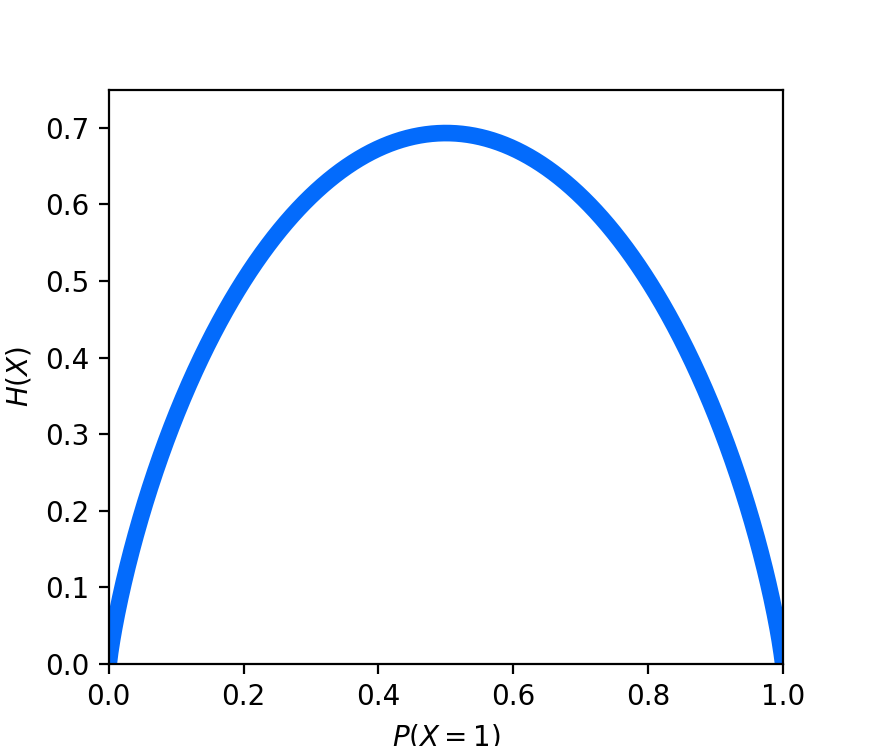
\includegraphics[width=4.5cm]{Plots/self-entropy.png}
    \caption{Shannon Entropy of a coin flip graphed versus the bias of the coin $P(x=1)$, where $x=1$ represents a result of heads.}
\end{figure}

\newpage
\subsection{Kullback-Leibler Divergence \& Cross-Entropy}

We can express cross entropy as the average number of bits needed to encode events from the true distribution $P(x)$ using the predicted distribution $Q(x)$. Cross-entropy is typically used as a loss function in supervised learning, aiming to minimize the difference between the predicted and true distributions. Cross-Entropy can also be seen as a way to measure the dissimilarity between two probability distributions for a given random variable or set of events.

$$H(P, Q) = - \mathbb{E}_{x \sim p} [{log Q(x)}] = -\int_x {P(x)log_2\left(Q(x)\right)dx} $$

\noindent If our predictions are perfect the predicted distribution is equal to the true distribution, then the cross-entropy is simply equal to the entropy. But if they differ then the cross-entropy will be greater than the entropy. 

$$ H(P, Q) \geq H(P) $$

\noindent The amount of bits which the Cross-Entropy exceeds the Entropy is called the relative entropy or the Kullback-Leibler Divergence. It quantifies how much extra information (in bits) is needed to encode events from one distribution when we use a code optimized for another distribution.

$$ D_{KL} (P \vert \vert Q) = H(P, Q) - H(P) = \mathbb{E}_{x \sim p} \left[ \frac{\log(P(x)}{\log(Q(x))} \right] = \mathbb{E}_{x \sim p} \left[ \log(P(x)) - \log(Q(x))  \right] $$

\noindent Because the KL divergence is non-negative and measures the difference between two distributions, it is often conceptualized as measuring some sort of distance between these distributions. However, it is not a true distance measure because is not symmetric.

$$ D_{KL} (P \vert \vert Q) \neq D_{KL} (Q \vert \vert P)$$

\noindent The KL divergence is 0 if P and Q are the same distribution (discrete variables) or equal almost everywhere (continuous variables).

\noindent Minimizing the Cross-Entropy with respect to Q is equivalent to minimizing the KL divergence between P and Q (if P is given, $H(P)$ and $ \mathbb{E}_{x \sim p} \left[ \log(P(x))  \right] $ are constants). In other words, given two distributions if one is fixed (your data-set) then you can only consider the approximation (your model).

\section{Maximum Likelihood Estimator}

In Deep Learning we work with parametric models that depend on a certain number of parameters (weights). The learning will consist then in trying to learn the correct weights. This can be seen as trying to find the parameters that maximize the likelihood that the training data is explained by the model probability distribution $p_{model}(x)$. Basically, among all the possible models we can choose, we will choose the one that explains the training data better. The maximum likelihood estimator for $\theta$ is defined as:

$$\theta_{ML} = argmax_{\theta} ~ p_{model} (x, \theta) $$

If the training data is a set of observations drawn i.i.d from an unknown data generative distribution $p_{data} (x)$ this can be written as:

$$\theta_{ML} = argmax_{\theta} \prod_{i=1}^{m} p_{model} (x^{(i)}, \theta) $$

\noindent Maximum Likelihood Estimator is a special case of Maximum a Posteriori Estimation when this one has a uniform prior. Basically, this consist in estimating the single set of parameters $\theta$ that maximize the likelihood that the model distribution $p_{model}(x)$ is able to explain the distribution of the training data. Conversely, using the Bayesian approach we will return a probability distribution over $\theta$ that characterize the likelihood of each set of possible parameters being able to explain the distribution of the training data. 

\noindent The Bayesian approach gives us a better estimate that Maximum Likelihood Estimator but is computationally extremely demanding. In the case of Neural Networks it is unfeasible to compute it (we have an infinite amount of hypothesis). Nevertheless, Maximum Likelihood Estimator is already a very good estimator. Having the assumption that the model of the true probability distribution is included in the hypothesis space, the Maximum Likelihood Estimator will converge to the optimal model.


\noindent Taking the product over many probabilities is numerically unstable. To solve that we can work with
the logarithm instead since it is a monotonically increasing function.

$$ \theta_{ML} = \log \left( argmax_{\theta} \prod_{i=1}^{m} p_{model} (x^{(i)}, \theta) \right) =  argmax_{\theta} \sum_{i=1}^{m} \log \left( p_{model} (x^{(i)}, \theta) \right)    $$

\noindent We can divide by m to express Maximum Likelihood Estimator as an expectation over the training data:

$$ \theta_{ML} = argmax_{\theta} ~ \mathbb{E} \left[ \log \left( p_{model} (x^{(i)}, \theta) \right) \right]    $$


\noindent Notice that this is result is equivalent to maximize the negative Kullback-Leibler divergence. We can see that
since the Kullback-Leibler divergence is given by:

$$ D_{KL} (p_{data} \vert \vert p_{model}) = \mathbb{E}_{x \sim p_{data}} \left[ \log(p_{data}(x)) - \log(p_{model}(x))  \right] $$

\noindent The term on the left is a function only of the data generating process therefore when we train the
model we only need to minimize.

$$- \mathbb{E}_{x \sim p_{data}} \left[ log \left( p_{model} (x) \right) \right] $$

\noindent Therefore can see the Maximum Likelihood Estimator as minimizing the Kullback-Leibler, which we know that is equivalent to minimizing the dissimilarity between the empirical data distribution $p_{data}(x)$ and the model distribution $p_{model}(x)$. Ideally, we would like to match the true data generating distribution $p_{data}$, but we have no direct access to this distribution.

\subsection{Condition Probability}

The probability of some event given that some other event has happened is called the conditional
probability and can be calculated as:

$$ P(Y=y \vert X=x) = \frac  {P(Y=y, X=x)} {P(X=x)} $$

\noindent Any joint probability distribution over many random variables may be decomposed into conditional
distributions over only one variable:

$$ P(x^{(1)}, ..., x^{(n)}) = P(x^{(1)}) \prod_{i=1}^{m} P(x^{(i)} \vert x^{(1)}, ..., x^{(i-1)})   $$

This is known as the chain rule or product rule of probability.

\subsection{Conditional Log-Likelihood}

The MLE can be generalized to the case where our goal is to estimate a conditional probability $ P (y \vert x, \theta)$
in order to predict $y$ given $x$.

$$\theta_{ML} = argmax_{\theta} ~ P (y \vert x, \theta) $$

\noindent If the input examples are i.i.d

$$\theta_{ML} = argmax_{\theta} ~ \sum_{i=1}^{m} P (y^{(i)} \vert x^{(i)}, \theta) $$

\subsection{Example: Linear regression as maximum likelihood}

Linear regression may be justified as a maximum likelihood procedure. Instead of producing a single prediction $\hat{y}$, we now think of the model as producing a conditional distribution $p(y \vert x)$. For linear regression we have the assumption to have Gaussian noise on the target with same variance, therefore the output will be the mean of a Gaussian distribution where the variance is fixed to some constant:

$$ p(y \vert x) = N(y, \hat{y}(x, \theta), \sigma^2)  $$

\noindent Considering the examples are assumed to be i.i.d.

$$\theta_{ML} = argmax_{\theta} ~ \sum_{i=1}^{m} P (y^{(i)} \vert x^{(i)}, \theta) = argmax_{\theta} ~ \sum_{i=1}^{m} N(y^{(i)}; \hat{y} (x^{(i)}, \theta), \sigma^2) = $$ 

$$ \theta_{ML} = argmax_{\theta} ~ \sum_{i=1}^{m} log \left( \sqrt{\frac{1}{2 \pi \sigma^2}}  \exp{\left[ -\frac{1}{2 \sigma^2} (y^{(i)} - \hat{y}^{(i)})^2  \right]}  \right) $$

$$ \theta_{ML} = argmax_{\theta} ~ \sum_{i=1}^{m} \left[ log \left( \sqrt{\frac{1}{2 \pi \sigma^2}} \right) + log \left(  \exp{\left[ -\frac{1}{2 \sigma^2} (y^{(i)} - \hat{y}^{(i)})^2  \right]}  \right)  \right] $$

$$ \theta_{ML} = argmax_{\theta} ~ \sum_{i=1}^{m} \left[ log (1) - log \left( \sqrt{2 \pi \sigma^2} \right) + \left( -\frac{1}{2 \sigma^2} (y^{(i)} - \hat{y}^{(i)})^2  \right)  \right] $$

$$ \theta_{ML} = argmax_{\theta} ~ \sum_{i=1}^{m} \left[ - \frac{1}{2} log  \left( 2 \pi \sigma^2 \right) + \left( -\frac{1}{2 \sigma^2} (y^{(i)} - \hat{y}^{(i)})^2  \right)  \right] $$

$$ \theta_{ML} = argmax_{\theta} ~   - \frac{n}{2} log  \left( 2 \pi \sigma^2 \right) +  \sum_{i=1}^{m} \left( -\frac{1}{2 \sigma^2} (y^{(i)} - \hat{y}^{(i)})^2  \right)   $$

$$ \theta_{ML} = argmax_{\theta} ~   - \frac{n}{2} log  \left( 2 \pi \sigma^2 \right) - \frac{1}{2 \sigma^2}  \sum_{i=1}^{m} \left(  y^{(i)} - \hat{y}^{(i)}  \right)^2   $$

\noindent Now we take out the part of the equation that does not depend on $\theta$.

$$ \theta_{ML} = argmax_{\theta} ~   - \sum_{i=1}^{m} \left(  y^{(i)} - \hat{y}^{(i)}  \right)^2   $$

\newpage
\noindent Which is equivalent to the Mean Squared Error formula used in regression which is:

$$ \theta_{MSE} = argmin_{\theta} ~ \frac{1}{n} \sum_{i=1}^{n} (y^{(i)} - \hat{y}^{(i)}(x, \theta) )^2 $$

\noindent To sum up we can say that maximizing the log-likelihood with respect to $\theta$ yields the same estimate of parameters $\theta$ as does minimizing the Mean Squared Error. That is why we use the Mean Squared Error as our loss function for regression problems.






    \chapter{Learning with Gradient}

\section{Gradient Descent}

Gradient Descent is a general approach to find the minimum of a differentiable convex function $J(\Vec{z})$ where $J (\Vec{z}): \mathbb{R} \rightarrow \mathbb{R} $ moving in the direction of the negative gradient. The Gradient Descent algorithm works as follows:

randomly initialize: $\Vec{z}~^{(0)}$

for $t = 1, ..., T$

~~~~~ $\Vec{z}~^{(t+1)} = \Vec{z}~^{(t)} - \eta \nabla(J(\Vec{z}~^{(t)})) $

output: $ \Vec{z}~^{(T)} $

\begin{figure}[h]
    \centering
    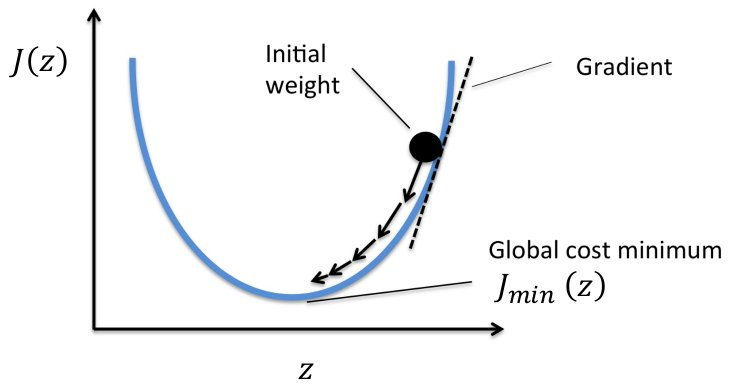
\includegraphics[width=10cm]{Images/gradient_descent.jpg}
    \caption{Gradient Descent algorithm update}
\end{figure}

where $\eta$ is the learning rate which indicates the size-step that we take at each update of the gradient.

\noindent The algorithm converges when the gradient is zero (or almost zero). Even though that in very simple cases we may be able to analytically solve $ \nabla J(\Vec{z}) = 0$ this is not the case for Deep Learning models. We have to keep in mind that in Deep Learning the loss function is often highly nonlinear and we also have a very large number of parameters which leads to having  many local minima and saddle points points. This means that even small changes in the weights can result in large changes in the loss function, making it difficult to determine the direction of steepest descent and find the global minima. 

Remember that in Machine Learning we don't have access to the real data distribution. Instead, the optimization is performed to an approximate function of the real distribution. For this reason, it doesn't matter that much to find the global minimum of a function that is not the real data distribution. We therefore usually settle for finding a value of f that is very low, but not necessarily minimal in any formal sense.

\newpage

\section{Jacobian and Hessian}

The Jacobian matrix is a matrix of first order partial derivatives that describes the rate of change of a multivariate function with respect to each of its input variables.
$$ f: \mathbb{R}^{m} \rightarrow \mathbb{R}^{n}, ~~ J \in \mathbb{R}^{n \times m} ~~~~ J = \left[ \frac{\partial f(x)}{\partial x_1}, ..., \frac{\partial f(x)}{\partial x_m}  \right] $$

\begin{figure}[h]
    \centering
    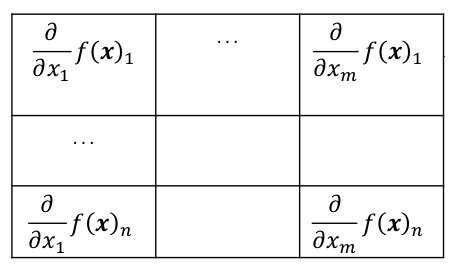
\includegraphics[width=7cm]{Images/jacobian.jpg}
    \caption{Jacobian Matrix}
\end{figure}

\noindent In Deep Learning the Jacobin matrix is used to update the computed minimum during the Gradient Descent algorithm.

\noindent Instead, the Hessian is a matrix of the second-order partial derivatives which describe the curvature of a multivariate function at a given point. It is the Jacobian of the gradient.

$$ f: \mathbb{R}^{n} \rightarrow \mathbb{R}, ~~ H \in \mathbb{R}^{n \times n} ~~~~ H_{ij} = \frac{\partial^2}{\partial x_i \partial x_j} f $$

\begin{figure}[h]
    \centering
    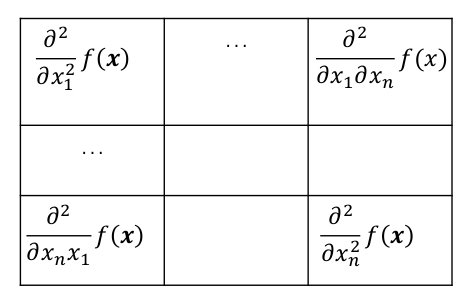
\includegraphics[width=7cm]{Images/hessian.jpg}
    \caption{Hessian Matrix}
\end{figure}

\noindent In the context of Deep Learning the Hessian is not very used as it is very expensive to compute. Nevertheless, second order methods have been proposed as an alternative to Gradient Descent. These ones have the advantage of knowing the direction in which the gradient is changing beforehand. This information can then be used to adjust the step size of the update rule making them converge more quickly and accurately to the local minimum than the Gradient Descent algorithm which operates only using first order derivatives.

\newpage
\subsection{Condition Number}

One application of the Hessian is computing the condition number. This is defined as a measure of the sensitivity of a function’s output to changes in its input and is calculated as the ratio of the maximum and minimum nonzero eigenvalues of the Hessian matrix.

$$ \left| \frac{ max(\lambda_i) }{min(\lambda_j)}  \right| $$


\noindent The condition number gives us information about the curvature in the different dimensions. A function with a high condition number indicates that the function has a large variation in its curvature, which can cause numerical instability, slow convergence and difficulty in finding the global minimum of the function. This is because in one direction the derivative increases rapidly, while in another direction it increases slowly. Therefore, the condition number can be used to diagnose if the the loss landscape is ill-conditioned which may lead to slow convergence or difficulties in optimization.


\begin{figure}[h]
    \centering
    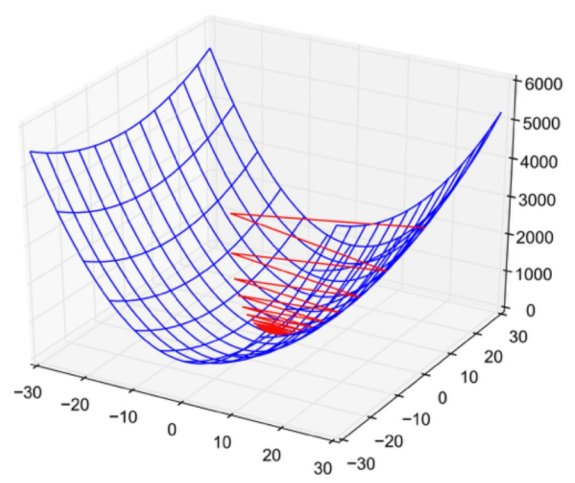
\includegraphics[width=7.5cm]{Images/condition_number.jpg}
    \caption{Condition Number}
    \label{fig:condition-number}
\end{figure}

\noindent In practise, the condition number is slow to compute since we need to calculate the Hessian beforehand. This is why is not so very used for Deep Learning. 
    \chapter{Neural Networks}

\section{Feed-Forward Neural Networks}

Feed-forward Neural Networks are described as a graph $G = (V, E)$ where $V$ are the vertices or neurons and $E$ are the edges, that is the connections between neurons. The edges are characterized by a weight $w$ which represents the strength of the connection between two neurons.

A Feed-forward Neural Network is organized in layers which contain a certain number of neurons. The first layer which takes as input the training data is called the input layer and the final layer that gives the output of the network is called the output layer. Between them we will have a certain number of hidden layers. The number of hidden layers and the neurons that each layer contain defines the architecture of the network.

\begin{figure}[h]
    \centering
    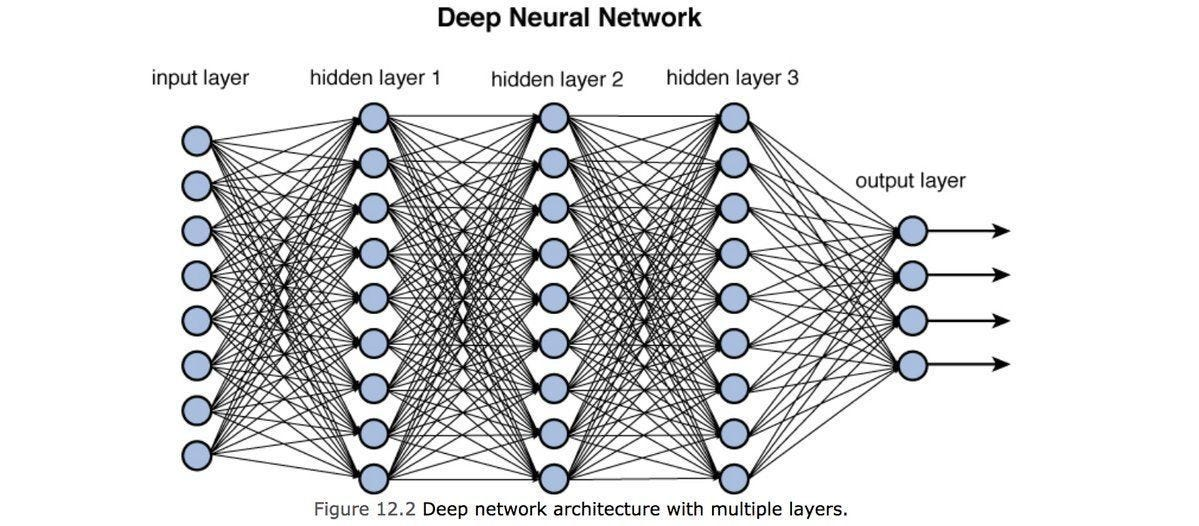
\includegraphics[width=14cm]{Images/feed-forward-nn.jpg}
    \caption{Feed Forward Neural Network architecture}
\end{figure}

\noindent In a Feed-forward Neural Network each neuron is connected to all the neurons of the previous layer, making a fully connected structure. Each neuron then takes as input the sum of the outputs of the connected neurons from the previous layer weighted by the edge weights and it applies to the result a non-linear activation function $\sigma$. The result gives that neuron output which will be used for computing next layer neurons. This process is repeated until reaching the output layer which will give us the network output.

Once the output is obtained we will compare the results with the labels or target of our data in order to calculate the loss. Once we done that we will be able to update the weights of our network and repeat the training process. This is done for $N$ epochs. The goal of the training is therefore learn the weights that best suits our problem.

\newpage
\noindent The simplest kind of Neural Network consists of only the input layer connected to a single unit that operates as the output. This kind of architecture is called a perceptron and is equivalent to simpler Machine Learning models such as logistic regression or Support Vector Machines in that they are only able to model functions which can linearly separate input data.

\begin{figure}[h]
    \centering
    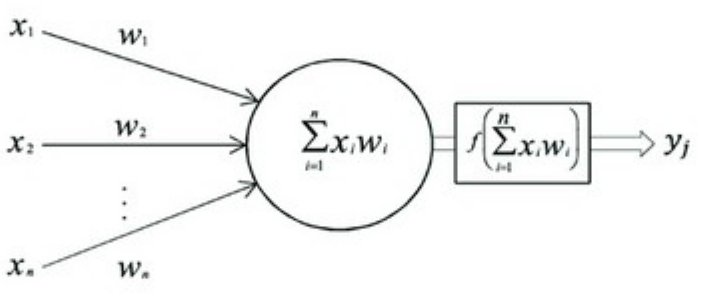
\includegraphics[width=7cm]{Images/perceptron.jpg}
    \caption{The perceptron is the simplest Neural Network architecture}
\end{figure}


\subsection{The Need for Deep Feed-Forward Neural Networks}

Shallow Deep Neural Networks have the same limitations as Machine Learning linear models, as they are not able to work with non-separable data. That's why we introduce non-linearity by means of introducing hidden layers and non-linear activation functions to the output of each neuron of the different hidden layers. This makes the model able to learn non-linear relationships in our data. For example we will only be able to solve the XOR task when we use at least one hidden layer in combination with a non-linear activation function to compute the values of the neurons. 

\begin{figure}[h]
    \centering
    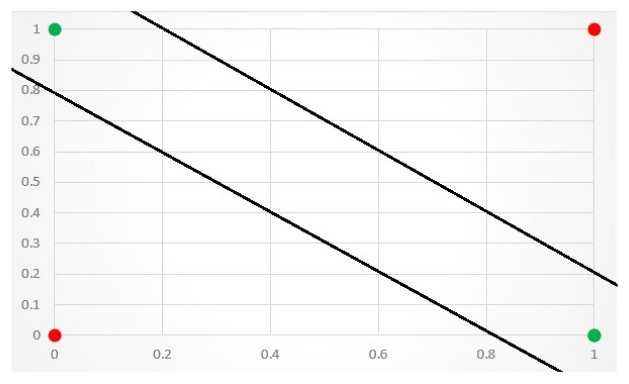
\includegraphics[width=8cm]{Images/xor.jpg}
    \caption{To solve the XOR problem we need to introduce non-linearity.}
    \label{fig:xor}
\end{figure}

\noindent Basically, the idea behind using multiple layers is that complex relations can be broken into simpler functions and combined. This makes our model able to learn more complex patterns in the data which will make it generalise better as the complexity of our model increases. This creates the necessity of using Deep Feed Forward Neural Networks, also called Multi-Layer Perceptrons which are represented as a composition of many different functions if we want to go further than Machine Learning linear models.

$$ f(x) = f^{(3)} \left(f^{(2)}\left(f^{(1)}\right)\right)$$

where $f^{(i)}$ represents the i-th layer.

\newpage
\section{Universal Approximation Theorem}

The Universal Approximation Theorem states that a feed-forward deep neural network with at least one hidden layer and a squashing (non-linear) activation function has the ability to approximate arbitrarily well any continuous function, given enough number of hidden units.

However, having a single hidden layer can require an exponential number of hidden units to approximate a given function with precision. This is why we usually build deeper layers, which will be able to learn more complex representations of our data making multi-layer Neural Networks preferable on practice. In fact, it has been shown that with the same number of parameters deeper networks tend to achieve a better result but at the same time they take more time to train.

Whichever the case there is not guaranteed that the training algorithm will be able to learn the continuous function we are targeting it. This is because the optimization algorithm may not be able to find the value of the parameters that corresponds to the desired function or the training algorithm might choose the wrong function (overfiting). 

\section{Gradient-Based Learning}

The largest difference between the linear Machine Learning models and Neural Networks is that the non-linearity of the network causes most loss functions to become non-convex. This leads to having no guarantee of achieving the global minimum. Therefore we will only be able to reach a local minima which makes our solution sensitive to the starting point.

The choice of the cost function is also an important aspect of the design of a Deep Neural Networks. In most cases, our parametric model defines a distribution $ p( y \vert x, \theta)$ and we simply use the principle of maximum likelihood. This means we use the cross-entropy between the training data and the model’s predictions as the cost function.

$$ J(\theta) = - \mathbb{E}_{x, y \sim p_{data}} \left[  log (p_{model} (y \vert x))  \right] $$

\noindent The specific form of the cost function changes from model to model, depending on the form of $log (p_{model})$. This makes the cost function choice tightly coupled with the choice of the output units.

\subsection{Linear Units for Gaussian Output}

If we set our outputs units to be linear units, this is equivalent to performing a regression task.

$$ \hat{y} = W^{T}h + b $$

\noindent In a regression task where the goal is to model the conditional distribution $p(y | x)$ it is common to use a Gaussian distribution.

$$ p_{model} (y \vert x) = N(y, \hat{y}, I)  $$

\noindent Because performing Maximum Likelihood Estimator in regression is equivalent to minimizing the Mean Squared Error. We will set the cost function as:

$$ J(\theta) = \frac{1}{2} \mathbb{E}_{p \sim p_{data}} \left[ ( y - f(x, \theta) )^2  \right] + constant  $$

using the Mean Squared Error as our cost function.

\newpage
\subsection{Sigmoid Units for Bernoulli Output Distributions}

Instead, in a binary classification problem the probability distribution is given by the Bernoulli distribution. This distribution is defined by a single parameter $\phi$.

$$P(x) = \phi^{x} \left(1 - \phi\right)^{1-x} $$

where  $\phi \in [0 ,1]$ and the Bernoulli distribution can only take two values: $P(x=1)=\phi$~ or ~$P(x=0)=1 - \phi$.

\noindent A Neural Network working in this framework should have as output the probability $\phi$ that given a data sample this belongs to one of the two classes. For example for class 1, this can be written as $P(y=1 | x) $. Since $\phi$ is a probability we should enforce this value to be inside the 0 to 1 range. This can be done by applying a non-linear activation function to the units output $\sigma \left(  w^Th + b \right)$. At the same time we want to ensure that the gradient is not 0 when the model is wrong. A very common choice that fulfills all these requirements is to use a sigmoid activation function which is defined as:

$$ \sigma (x) = \frac{1}{1 + exp(-x)} $$

\noindent We can demonstrate that the sigmoid function is the reasonable choice by operating in the following way. Defining

$$ z = w^T h + b$$

\noindent Then we made the assumption that we can define an unnormalized probability $\hat{P}(y)$ as

$$ \log \left( \hat{P}(y) \right) = yz ~~~ \rightarrow ~~~ \hat{P}(y) = exp(yz) $$

\noindent We can then get the normalize probability $P(y)$ by doing

$$ P(y) = \frac{exp(yz)}{\sum_{y'=0}^{y'=1} exp(y'z)} = \sigma \left( (2y -1)z \right)$$

\noindent Taking into account that the cost function used with maximum likelihood is $-log \left(P(y|x) \right)$ we get:

$$ J(\theta) = - log \left( P(y | x) \right) = - log \left( \sigma \left( (2y -1) z \right) \right) = \zeta \left( \left( 1 -2y \right) z \right)$$

where $\zeta (x) = \log \left( 1 - \exp{(x)} \right)$

\noindent Using sigmoid, saturation will occur when $y=1$ and $z$ is very positive or when $y=0$ and $z$ is very negative. Basically when the model has the right answer that is what we are looking for.

\noindent If we apply other loss loss function like Mean Squared Error, the model will still able to learn but because we are not following the Maximum Likelihood Estimator when operating with a binary classifier it will converge to a worse solution than when using a sigmoid units.

\subsection{Softmax Units for Multinoulli Output Distributions}

To generalize to the case of a discrete variable with $n$ values, we now need to produce an output vector $\hat{y}=[ \hat{y}_0, \hat{y}_1,... , \hat{y}_{n - 1}]$ where $ \hat{y}_i = P(y=i \vert x) $ and we require that:

$$ \forall ~ i ~~ 0 \le \hat{y}_i \le 1   ~~~ \sum_{i} \hat{y}_i = 1 $$

\newpage
\noindent The same approach that worked for the Bernoulli distribution generalizes to the multinoulli distribution. First, a linear layer predicts the un-normalized log probabilities:

$$ z = W^T + b $$

where $ z_i = \log P(y=i \vert x)$. The soft-max function can then exponentiate and normalize $z$ to obtain the desired $\hat{y}$. Formally, the softmax function is given by

$$ softmax (z_i) = \frac{exp(z_i)}{\sum_j exp(z_j)}   $$

\noindent As with the logistic sigmoid, the use of the exponential function works very well when training the softmax to output a target value y using maximum log-likelihood. Defining the softmax in terms of the exponential is natural because the log in the log-likelihood can undo the exponential of the softmax:

$$\log softmax (z)_j = z_i - \log \sum_j \exp{(z_j)}  $$

where the first term $z_i$ encourages the model to increase the output of the correct labels and the second term encourages the model to decrease the output of incorrect labels.

\section{Hidden Units}

Contrary to the output units where we choose the activation function following the maximum likelihood estimator principle, in hidden units there is not a way to define these activation functions beforehand. Nevertheless, a good principle is to use ReLU as a default. This is because linear models are the simplest to optimize. As a result ReLU and their variants, that are still non-linear but have a part of the function that behave linearly, are considered the way to go. More complex activation functions like sigmoid or $\tanh (x)$ can learn a more complex representation of the data as the hypothesis space will be bigger but at the same time they tend to overfit more and are more difficult to optimize. In any way, we will need to perform trial an error between a sample of activation functions in our hidden units to choose the one that works best.


    \chapter{Back-propagation}

When training a Neural Networks we have two phases: forward propagation and back-propagation. In the forward propagation phase, the input goes through the network producing the network output $\hat{y}$. Given an input x and a neural network with L layers, the forward pass can be expressed as follows: 

Input: $a^{(0)} = x$

For each layer l from 1 to L: $ z^{(l)} = W^{(l)}a^{(l-1)} + b^{(l)}  ~~~~  a^{(l)} = \sigma (z^{(l)}) $

Where $z^{(l)}$ is the weighted sum at layer l, $a^{(l)}$ is the activation (output) at layer l and $\sigma$ is the activation function. At the output layer $a^{(L)} = \hat{y} $

\noindent Using then the targets $y$ of the training data, we will be able to compute the cost function $J(\theta)$ which indicates the amount of error our network makes. The choice of cost function $J(\theta)$ depends on the specific problem. For example, for binary classification, you might use cross-entropy loss:

$$J(\theta) = - \frac{1}{m} \sum_{i=1}^m \left[ y^{(i)}\log(\hat{y}^{(i)}) + (1 - y^{(i)})log(1 - \hat{y}^{(i)}) \right]$$


\noindent In order to correct our network so it can learn a parameter set that returns a lesser amount of error we will perform back-propagation. This process consists of computing the gradients of the loss function during the backward pass of training. This determines how much each parameter (weights and biases) contributed to the error in the network's prediction. These gradients, calculated using the chain rule of calculus, guide the adjustments of network parameters to minimize the loss.

The gradients of the cost with respect of the weighted sum $z^{(l)}$: $\delta^{(l)} = \frac{\partial J}{\partial z^{(l)}} $

Gradients of the cost with respect to the weights $ W^{(l)} $: $ \frac{\partial J}{\partial W^{(l)}} = \delta^{(l)}(a^{(l-1)})^{T} $

Gradients of the cost with respect to the biases $ b^{(l)} $: $ \frac{\partial J}{\partial b^{(l)}} = \delta^{(l)} $


\noindent Now in order to update those parameters we will need to use an optimization algorithm that updates the network parameters iteratevely in the direction that minimizes the cost function. One of the most common algorithms used to do that is stochastic gradient descent which is a modification of vanilla gradient descent but instead of working with the whole dataset at each iteration it uses a fraction of it. This makes the algorithm more stochastic but at the same time more fast to converge as well as be able to escape saddle points and local minima more easily. SGD therefore efficiently navigates the parameter space to find optimal values by iterating this process a number of N epochs.

$$ W^{(l)}_{t+1} = W^{(l)}_{t} - \eta \frac{\partial J}{\partial W^{(l)}_{t}} ~~~~~ b^{(l)}_{t+1} = b^{(l)}_{t} - \eta \frac{\partial J}{\partial b^{(l)}_{t}} $$



    \chapter{Regularization}

Deep Neural Networks tend to represent very complex functions which leads to overfitting the training data (variance in the estimator). Therefore, most regularization strategies are based on regularizing estimators which trades bias for a reduced variance. Additionally, regularization will also reduce the capacity of the model. The learning bias will favour simpler hypothesis.

\section{Parameter Norm Penalties}

We can perform regularization by adding a parameter norm penalty $\Omega(w)$ that limits the capacity of the model to the cost function J.

$$ J(w, X, y) + \alpha \Omega (w) $$

Where $\alpha$ is a hyper-parameter that weights the relative contribution of the norm penalty term, $\Omega$ relative to the standard cost function J. A larger $\alpha$ then will result in more regularization.

\begin{figure}[h]
    \centering
    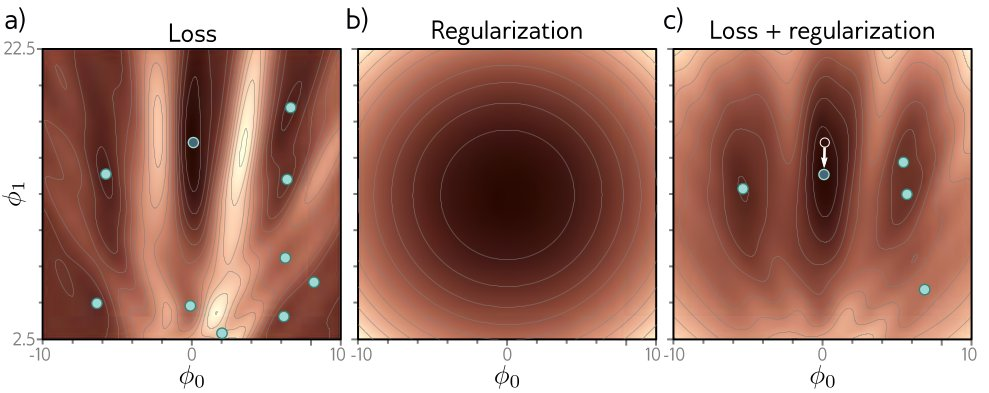
\includegraphics[width=12cm]{Images/parameter-norm.jpg}
    \label{fig:parameter-norm}
\end{figure}

\subsection{L2 Parameter Regularization}

The L2 parameter norm penalty, also known as weight decay drives the weights closer to the origin by adding a regularization term to the cost function.

$$ \Omega(w) = \frac{1}{2} || w ||_{2}^{2} $$

\noindent If we remember, Maximum Likelihood Estimator was an special case of Maximum a Posteriori Estimation when we had a uniform prior. By adding a regularization parameter to the cost function we are changing the prior distribution to a Gaussian prior centered on 0 where the hyperparameter $\alpha$ acts like the variance. In this way we are favouring the hypothesis inside our hypothesis space that have smaller weights.

\newpage
\noindent Performing the gradient adding to the cost function the L2 norm is known as ridge regression or Tikhonov regularization. 

$$\Tilde{J} (w, X, y) = \frac{\alpha}{2} w^T w + J(w, X, y) ~~~~~ \nabla_w \Tilde{J} (w, X, y) = \alpha w + \nabla_w J (w, X, y)$$

\noindent The addition of the weight decay term will modify the learning rule to shrink the weight vector by a constant factor on each step, just before performing the usual gradient update.

$$ w \leftarrow w - \epsilon \left( \alpha w + \nabla_w J(w, X, y) \right) ~~~~~  w \leftarrow (1 - \epsilon \alpha) w - \epsilon \nabla_w J(w, X, y) $$

\subsection{L1 Parameter Regularization}

Another option is to use L1 regularization which is defined as:

$$ \Omega (w) = ||w||_1 $$

\noindent In comparison to L2 regularization, L1 regularization results in a solution that is more sparse. Sparsity refers to the fact that some parameters have an optimal value of zero making L1 regularization fitting for use in feature selection.

\noindent The gradient now will be.

$$ \nabla_w  \Tilde{J} (w, X, y) = \alpha sign(w) + \nabla_w J (w, X, y)$$

Notice how the weights $w$ are pushed to 0 by adding $\alpha sign(w)$ to the gradient.




\begin{figure}[h]
    \centering
    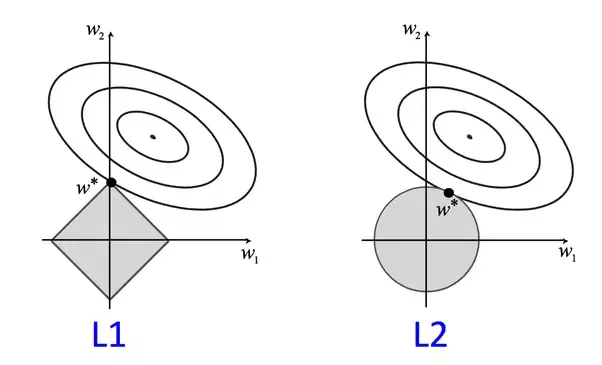
\includegraphics[width=6cm]{Plots/parameter_regularization.png}
    \caption{L1 and L2 regularization behaviour}
    \label{fig:parameter-regularization}
\end{figure}

\section{Other Regularization Techniques}

\subsection{Data Augmentation}

The best way to make a model generalize better is to train it on more data. In case we cannot gather more data, we can apply a small transformation to the training data generating fake data in the process which we will be able to add it to the training set. This technique is called data augmentation. Dataset augmentation has been particularly effective for object recognition. Creating new samples rotating, translating or scaling our images will ensure that the model is invariant to rotations, translations and scaling transformations making it to generalize better.


\subsection{Transfer Learning (Pre-training)}

Transfer learning is a regularization technique used when the training data is limited. It involves training a neural network on a related secondary task for which data are more plentiful. The network learns valuable features from this secondary task, which can later be utilized to improve performance on the original task. Basically, transfer learning can be seen as initializing most of the parameters of the final network in a sensible part of the space that is likely to produce a good solution.

\newpage

\subsection{Multi-task Learning}

Multi-task learning involves training a single neural network model using examples from multiple related tasks. The model then will have both task-specific and generic parameters. The shared layers captures common patterns and makes the model able to learn a representation that generalizes well.
Meanwhile, the task-specific layers handle task-specific details. Multi-task learning improves performance by leveraging knowledge from multiple tasks and benefiting from shared representations.

\begin{figure}[htp]
    \centering
    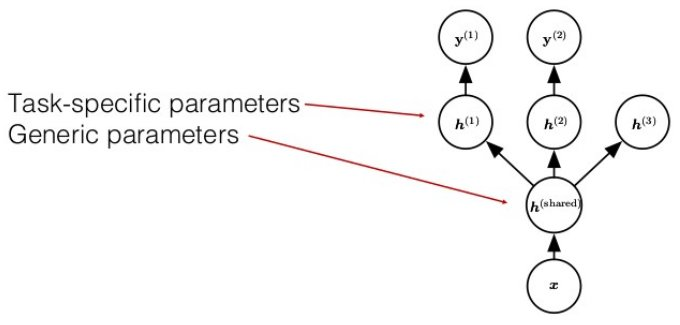
\includegraphics[width=10cm]{Images/multi-task_learning.jpg}
    \caption{Multi Task Learning}
    \label{fig:muti-task_learning}
\end{figure}

\subsection{Self-Supervised Learning}

When data from other tasks is not available, self-supervised learning can be used to create large amounts of “free” labeled data and use it for transfer learning. There are two types of self-supervised learning: Generative and Constrastive.

\begin{itemize}
    \item Generative Self-supervised Learning: Part of each data sample is masked and the secondary task is predicting missing parts in masked data.
    \item Constrastive Self-supervised learning: Two versions of each unlabeled example are presented, where one has been distorted in some way. The system is then trained to predict which is the original.
\end{itemize}

\noindent These techniques help the network learn representations that can be transferred to the primary task, enhancing performance without task-specific labeled data.

\begin{figure}[h]
    \centering
    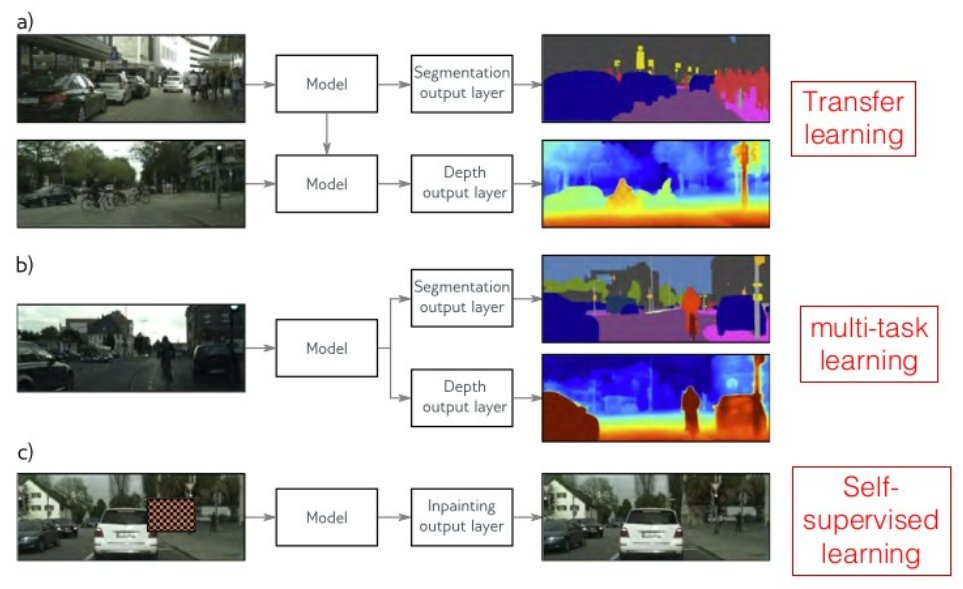
\includegraphics[width=13cm]{Images/self-supervised_learning.jpg}
    \caption{Self-Supervised Learning}
    \label{fig:self-supervised}
\end{figure}

\subsection{Early Stopping}

When training large models these ones may overfit as the number of epochs go by. We often observe that training error decreases steadily over time, but the validation set error begins to rise again.

\begin{figure}[htp]
    \centering
    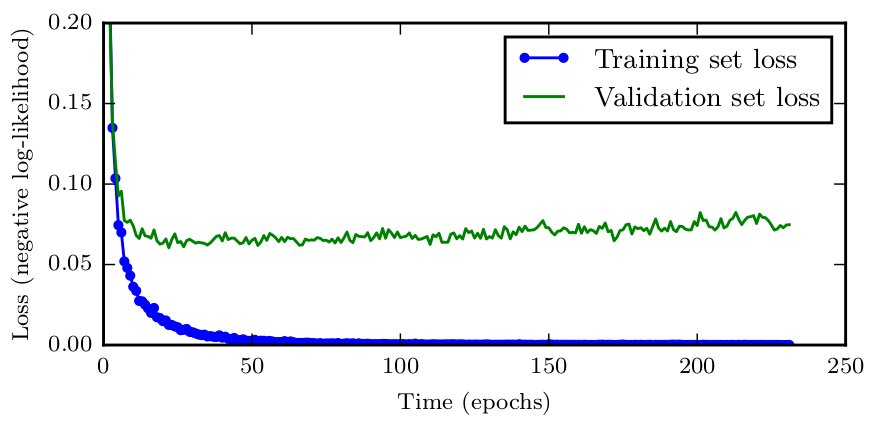
\includegraphics[width=7.5cm]{Plots/early-stopping.jpg}
    \caption{Early Stopping}
    \label{fig:early-stopping}
\end{figure}

\noindent What we can do is to stop the training algorithm once we see no improvement for N epochs. This technique is called early stopping. We will therefore regularize the model as it limits the parameter space to a neighborhood of the initial parameter values.

\subsection{Bagging and Boosting}

Bagging is a technique for reducing generalization error by combining several models. The idea is to train several different models separately with different subsets of the data through sampling with replacement, then have all of the models vote on the output for the test examples. On the other hand, boosting works in the opposite direction. Instead of reducing variance, boosting builds an ensemble with higher capacity. In boosting, each model is trained iteratively, with subsequent models focusing on the examples that were previously misclassified by earlier models. By giving more weight to difficult examples, boosting aims to improve the overall performance of the ensemble. Examples: AdaBoost and XGBoost. Training different models and using ensembles, such as bagging and boosting, improve performance by reducing errors and increasing model diversity.


\begin{figure}[h]
    \centering
    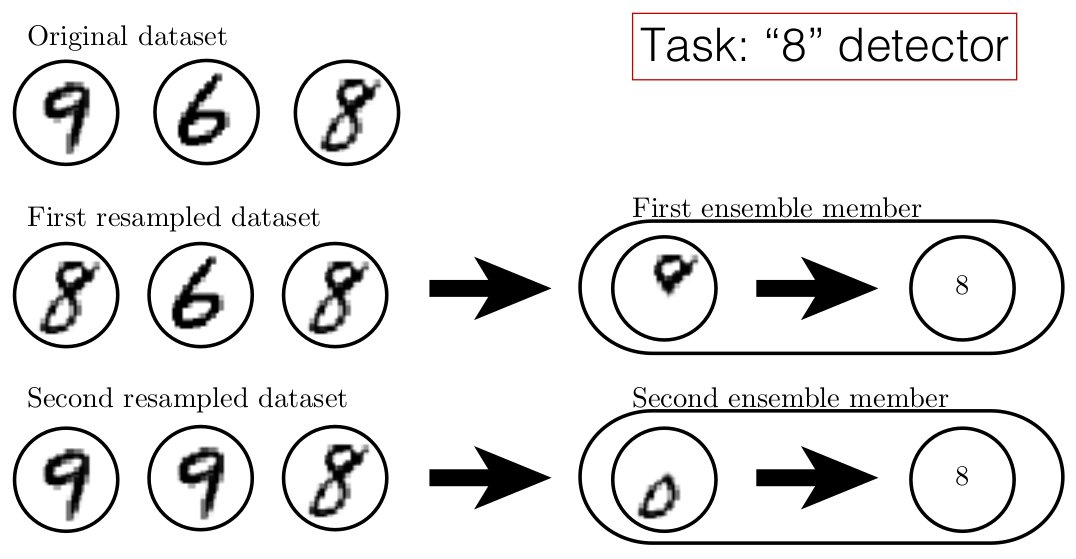
\includegraphics[width=10cm]{Images/bagging.jpg}
    \caption{Caption}
    \label{fig:bagging}
\end{figure}

\newpage
\subsection{Dropout}

Dropout is an efficient regularization technique used in Neural Networks that involves randomly removing units from the network during training using binary masks which silences some neurons. This creates an ensemble of sub-networks. Therefore, dropout can be seen as a way to perform an ensemble method on a Deep Neural Network. Each sub-network inherits a different subset of parameters from the parent network. This process approximates the idea of training multiple independent models in bagging. Basically, we reduce the generalization error by combining several models. The idea is to train several different models separately, then have all of the models vote (or take the mean of them) on the output for the test examples. This process helps in reducing overfitting and introducing regularization to the network.

\begin{figure}[h]
    \centering
    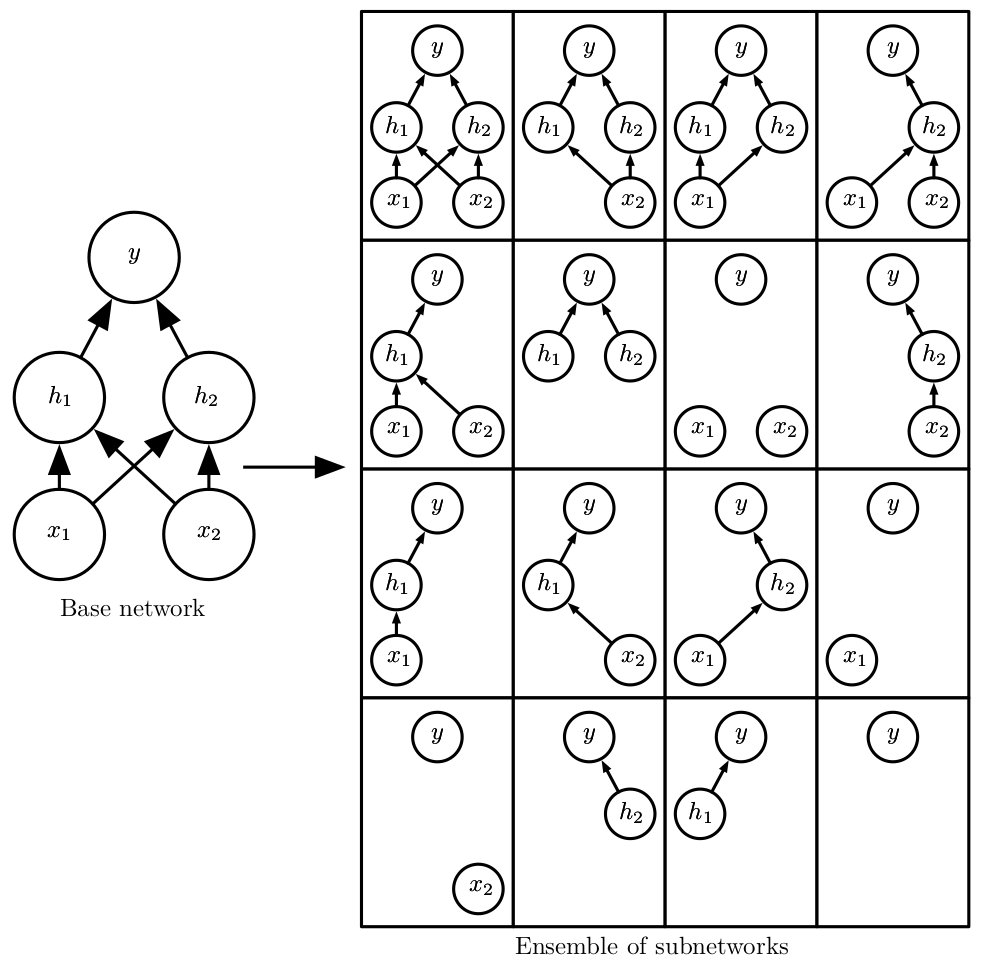
\includegraphics[width=10cm]{Images/dropout.jpg}
    \caption{Dropout ensemble of networks}
    \label{fig:dropout}
\end{figure}

\noindent Dropout then is able to reduce overfitting by considering simpler models of our DNN but constructing many of them so the errors of one model will not be repeated by the others. This is a strategy to reduce the variance of the NN trading it with bias.

\noindent During evaluation, dropout is not applied. Instead, the full network is used for predictions. However,
the weights of the neurons are scaled down by the dropout probability to account for the fact that,
on average, fewer neurons were active during training. This scaling ensures that the expected output
of the neurons remains the same, maintaining consistency between training and evaluation.

\newpage
\subsection{Adversial Training}

Adversarial training introduces adversarial samples that are intentionally crafted input data slightly perturbed to mislead the model’s prediction. These are samples constructed by using an optimization procedure to search for an input $x'$ near a data point $x$ such that the model output is very different at $x'$.

\begin{figure}[h]
    \centering
    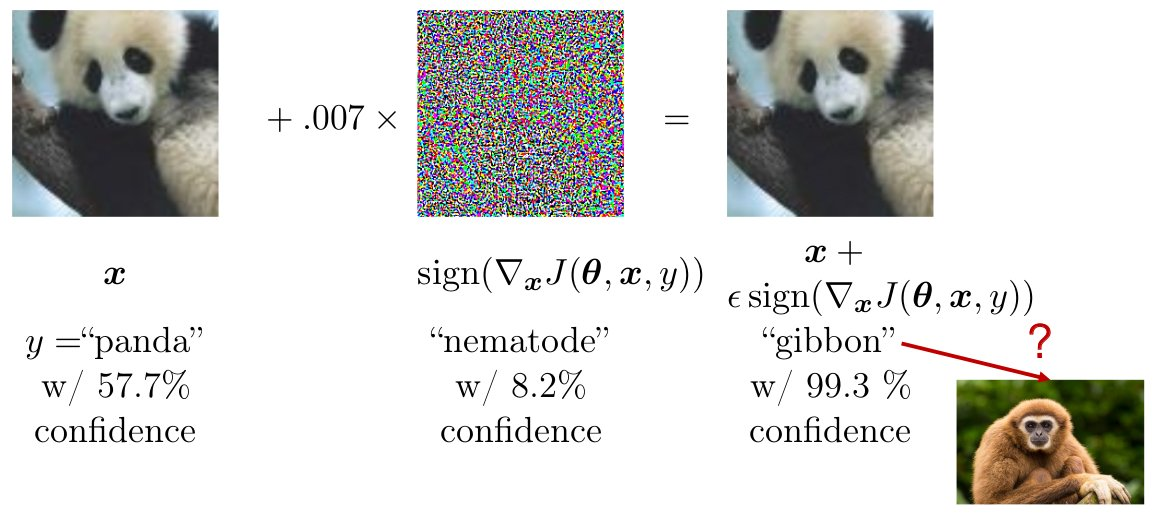
\includegraphics[width=12cm]{Images/adversarial-training.jpg}
    \caption{Caption}
    \label{fig:enter-label}
\end{figure}

\noindent The addition of adversarial examples introduces a form of regularization by effectively expanding the training distribution to include adversarial instances. This helps prevent overfitting in the training set and encourages the model to learn more robust and generalizable features.



    \chapter{Optimization}

In optimization the goal is to optimize a performance measure. Ideally we should aim to optimize the true error but in Machine Learning the true error is not computable.

$$J(\theta) = \mathbb{E}_{(x, y) \sim S} L(f(x, \theta), y) = \frac{1}{n} \sum_{i=1}^{n} L(f(x^{(i)}, \theta), y^{(i)})$$

where S is the sample data that we have in our dataset. If the sample size is large enough the true error and the empirical error are approximately the same. However, this approach can lead to overfitting, where the model memorizes the training data rather than generalizing. Additionally, many loss functions used in deep learning are not differentiable (e.g. 0-1 Loss), making it difficult to employ gradient descent. Therefore, we will require specialized techniques and novel approaches to effectively train neural networks such as using a surrogate loss (e.g. negative log likelihood as surrogate for 0-1 loss) that can be used together with gradient descent.

\section{Batch/Mini-batch Algorithms}

A common optimization technique are the the batch/mini-batch algorithms. These are divided depending on the amount of the original data that we use.

\begin{itemize}
    \item Batch or Deterministic Gradient Descent: This algorithm computes the gradient of the loss on the whole training set and then updates the weights. Therefore it has the advantage of computing the right gradient but on the other hand it will be very costly and slow. It will also only update the weights one time per epoch.
    \item Online or Stochastic Gradient Descent: This algorithm computes the gradient of the loss on a single sample on the training set and then updates the weights. This has the advantage of performing a weight update once per sample (we will do n updates per epoch where n is the data size). On the other hand, the gradient is less accurate since it computes the gradient of the loss only with respect to a single example.
    \item Mini-batch Stochastic Gradient Descent: This algorithm is a compromise between the last two methods. It computes the gradient of the Loss on a subset of examples (mini-batch) of the training set and then updates the weights. This approach provides a compromise between the accurate gradient computation of batch gradient descent and the increased number of weight updates of stochastic gradient descent.    
\end{itemize}

\noindent Overall this technique reduces the computational cost and has a regularization effect (noise in the gradient). Therefore, the algorithm will converge faster at the expense of using less accurate gradient estimations with respect to the exact gradient.

\newpage

\section{Challenges in Optimization}

The most prominent challenges involved in optimization for training deep models are:

\subsection{Ill-Conditioning of Hessian}

Ill-conditioning of the Hessian matrix occurs when the second derivatives have a large variance, making it difficult for first-order methods like Stochastic Gradient Descent to converge. If the function to optimize resembles a long canyon (the direction with most curvature has way more curvature than the direction with the least curvature) there will be an inefficient zigzagging while performing the SGD algorithm which wastes time and slows down the convergence of the optimization algorithm.

\begin{figure}[h]
    \centering
    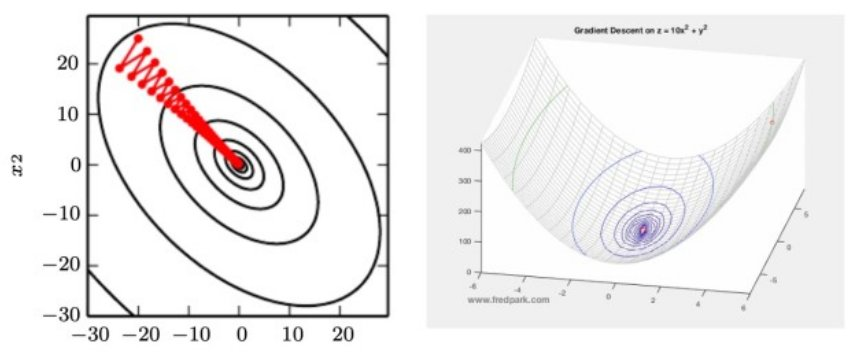
\includegraphics[width=10cm]{Plots/ill-conditioned-hessian.jpg}
    \caption{Zig-zagging of the gradient in a ill conditioned Hessian}
\end{figure}

\subsection{Saddle Points and Local Minima}

Because in Neural Networks training we are dealing with a non-convex cost function we will have many non-optimal local minima due to symmetries and weight scaling. In the past this used to be considered a major problem in Deep Learning but nowadays is has been shown that  it is sufficient to find a point with low cost as different parameter configurations can achieve similar performance. Additionally, in high-dimensional spaces, saddle points are more common than local minima. This is because saddle points have a mix of positive and negative eigenvalues in their Hessian matrix, while local minima have only positive eigenvalues. In a n-dimensional space it is exponentially unlikely that all eigenvalues are positive.

\begin{figure}[h]
    \centering
    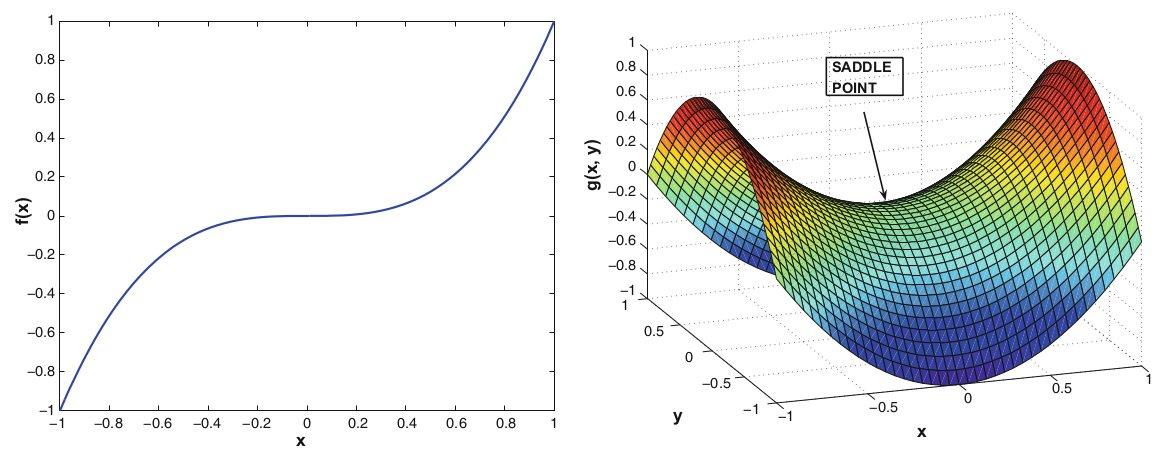
\includegraphics[width=10cm]{Plots/saddle-point.jpg}
    \caption{Example of 1 dimensional and 2 dimensional saddle points.}
\end{figure}

\noindent Saddle points can also pose challenges for optimization algorithms. First-order methods like Stochastic Gradient Descent has proven to be able to escape saddle points quickly due to the small gradient near them. In contrast, second-order methods may jump to saddle points. This is why first-order methods are preferred for training deep neural networks.

\newpage

\subsection{Flat Regions}

Flat regions, where both the gradient and the Hessian are close to zero, makes it difficult for the algorithm to determine the direction of improvement and navigate towards better solutions.

\begin{figure}[h]
    \centering
    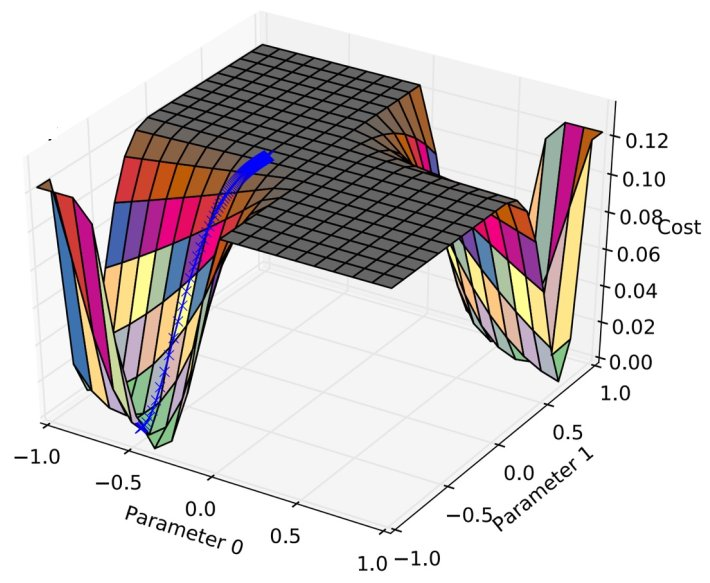
\includegraphics[width=6.5cm]{Plots/flat-regions.jpg}
    \caption{Example of a 2 dimensional flat region}
\end{figure}

\subsection{Cliffs and Exploding Gradients}

Deep Neural Networks may have extremely steep regions called cliffs which cause the gradient to become large, resulting in weight updates that jump far away. To mitigate the issues caused by exploding gradients and the instability they introduce, a technique called gradient clipping is often employed. This one consists in limiting the magnitude of the gradient, preventing it from growing too large. By reducing the step size, gradient clipping helps stabilize the training process and prevents weight updates from taking excessively large leaps.

\begin{figure}[h]
    \centering
    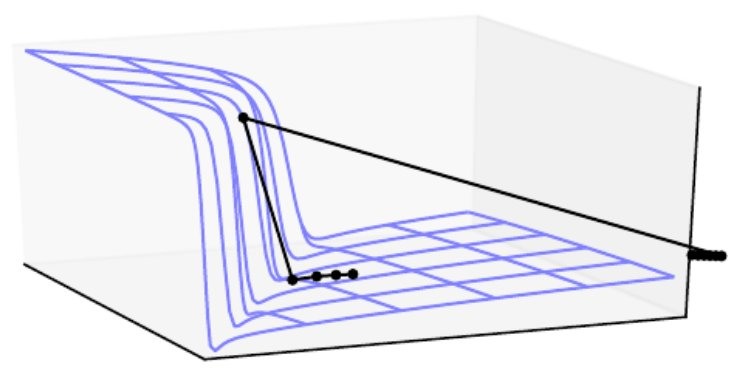
\includegraphics[width=6.5cm]{Plots/cliffs.jpg}
    \caption{Example of a cliff in gradients}
    \label{fig:gradient-cliff}
\end{figure}

\subsection{Exploding/Vanishing Gradients}

Another problematic challenge is the issue of exploding and vanishing gradients. This happens in Recurrent Neural Networks due to repeatedly multiply the input by the weight matrix $W$.

$$ W = V diag(\lambda) V^{-1} $$

\noindent Multiplying this matrix $t$ times we end up with.

$$W^{t} = V {diag(\lambda)}^t V^{-1}$$

\noindent If the eigenvalues are not close to 1, they will either vanish (eigenvalues << 1) or explode (eigenvalues >> 1). Cliffs are an example of exploding gradients.

\noindent We will have a similar problem with activation functions that can saturate (e.g sigmoid) which will produce a vanishing gradient. However, feed-forward networks with non-saturating activation functions, like ReLU, and different matrices for each layer, avoid this problem.

\newpage

\section{Stochastic Gradient Descent}

Stochastic Gradient Descent is a variation of Gradient Descent that makes use of a mini-batch m to compute the gradient instead of the whole dataset (making it less computationally expensive). This introduces noise which makes the algorithm more able to escape from local minimum and saddle points. Therefore, Stochastic Gradient Descent is in general a more robust algorithm and can reach better solutions compared with vanilla Gradient Descent. Another difference is that we have an adaptative learning rate $\eta$. The Stochastic Gradient Descent algorithm updates the $W$ parameters of layer $l$ as follows:

$$ W_{t+1}^{l} = W_{t}^{l} - \eta \frac{\partial J}{\partial W_{t}^{l}} $$

\subsection{Momentum}

Stochastic Gradient Descent can be slow, so in order to speed up the training a momentum is introduced. Momentum therefore helps accelerate convergence, especially in cases where the loss landscape has irregularities or noisy gradients. The Stochastic Gradient Descent algorithm with momentum is as follows:

$$ v = \beta v - \eta \frac{\partial J}{\partial W_{t}^{l}}  ~~~  W_{t+1}^{l} = W_{t}^{l} + v $$

\noindent The momentum is initialized at 0 since at the beginning of the optimization process, there is no accumulated momentum from previous iterations. The momentum term $\beta$ is a value between 0 and 1 (usually is set to 0.9). 

Introducing momentum produces that the gradient in one direction is increased if all these gradients are aligned over multiple iterations but decreased if the gradient direction repeatedly changes. The overall effect is a smoother trajectory and reduced oscillatory behavior in valleys making the algorithm able to navigate noisy or small gradients more efficiently, leading to faster convergence.

\subsection{Nesterov Momentum}

Another optimization algorithm that introduces a variance of momentum is called the Nesterov momentum. The Stochastic Gradient Descent algorithm is now:

$$ \tilde{W}_{t}^{l} = W_{t}^{l} + v $$

$$ v = \beta v - \eta \frac{\partial J}{\partial \tilde{W}_{t}^{l}}  ~~~~~  W_{t+1}^{l} = W_{t}^{l} + v $$

\noindent In Nesterov momentum the gradient is evaluated after the current velocity is applied. Thus one can interpret Nesterov momentum as attempting to add a correction factor to the standard method of momentum.

\section{Parameter Initialization}

Parameter initialization is a crucial step on our Deep Neural Network models as these ones are very dependent on the initialization points. Bad initial points can cause numerical instabilities and algorithm failure. In the general case where various activation functions like sigmoid or tanh are used, initializing all weights to zero is problematic because it leads to the symmetry problem. Basically, when all weights in a layer are the same, neurons compute identical functions and they will evolve into the same values, resulting in redundant behavior. The layer will be equivalent to a layer with only one neuron. Breaking symmetry with proper initialization ensures stable training and a better generalization.

\noindent On the other hand, when using the ReLU activation function, although this one avoids the symmetry problem, initializing all weights to zero is neither a a good idea. In a network with ReLU activations, neurons with zero weights (or weights that become zero after initialization) will always output zero for any input during forward propagation. This leads to the problem of "dead neurons". Dead neurons cannot recover during training because their gradients are always zero (due to the ReLU derivative being zero for negative inputs). Having a significant number of dead neurons can severely limit the expressive power of the network and lead to suboptimal performance. It essentially reduces the network's capacity to represent complex functions and patterns in the data.

A common strategy is to initialize the weights randomly taking the values from a Gaussian or uniform distribution. Keep in mind that large weights can cause issues like exploding values or gradient saturation. Therefore, it is common to initialize weights close to zero with a specific scale. For fully connected layers with m inputs and n outputs heuristics like the uniform distribution are used.

$$ W_{i, j} \sim U \left(  \frac{-1}{\sqrt{m}}, \frac{1}{\sqrt{m}} \right) $$


\noindent Biases are often initialized with pre-defined constants to avoid saturation (usually 0 or 0.1 for ReLU to avoid saturation).

\section{Algorithms with Adaptative Learning Rates}

Gradient Descent algorithm with a fixed step size has an undesirable property: it makes large adjustments to parameters associated with large gradients and small adjustments to parameters associated with small gradients. A number of mini-batch-based algorithms have been introduced that adapt the learning rates of model parameters.

\subsection{AdaGrad}

AdaGrad is an optimization algorithm that scales learning rates inversely proportional to the square root of the sum of all of their historical squared values. The parameters with the largest partial derivative of the loss have a correspondingly rapid decrease in their learning rate, while parameters with small partial derivatives have a relatively small decrease in their learning rate. The net effect is greater progress in the more gently sloped directions of parameter space.

\noindent We update the accumulator as:

$$ G_{t}^{l} = G_{t-1}^{l} + \left( \frac{\partial J}{\partial W_{t}^{l}}  \right)^2  $$

\noindent Update the weights:

$$ W_{t+1}^{l} = W_{t}^{l} - \frac{\eta}{\sqrt{G_{t}^{l} + \delta}} \frac{\partial J}{\partial W_{t}^{l}} $$

\subsection{RMSProp}

In AdaGrad, the accumulation from the beginning of the training results in an excessive decrease in the learning rate. The RMSProp algorithm modifies AdaGrad to solve this issue by changing the gradient accumulation into an exponentially weighted moving average. The idea is to only converge rapidly after finding a convex bowl.

\noindent We update the accumulator as:

$$ G_{t}^{l} = \beta G_{t-1}^{l} + (1 - \beta) \left( \frac{\partial J}{\partial W_{t}^{l}}  \right)^2  $$

\noindent Update the weights:

$$ W_{t+1}^{l} = W_{t}^{l} - \frac{\eta}{\sqrt{G_{t}^{l} + \delta}} \frac{\partial J}{\partial W_{t}^{l}} $$


\subsection{Adam}

Adam combines the benefits of both the AdaGrad algorithm and RMSprop. Adam maintains adaptive learning rates for individual parameters by using estimates of first and second moments of the gradients:

\noindent We update the biased first moment estimate as:

$$ s = \beta_{1}s + (1 - \beta_{1})\frac{\partial J}{\partial W_{t}^{l}} $$

\noindent We update the biased second moment estimate as:

$$ r = \beta_{2}r + (1 - \beta_{2})\left( \frac{\partial J}{\partial W_{t}^{l}}  \right)^2 $$

\noindent Correct the bias in the first moment:

$$ \tilde{s} = \frac{s}{1 - \beta_{1}^{t}} $$

\noindent Correct the bias in the second moment:

$$ \tilde{r} = \frac{r}{1 - \beta_{2}^{t}} $$

\noindent Update the weights:

$$ W_{t+1}^{l} = W_{t}^{l} -\eta \frac{\tilde{s}}{\sqrt{\tilde{r}} + \delta}   $$


where $\beta_{1}$ and $\beta_{2}$ are the exponential decay rates for moment estimates. Usually their values are 0.9 and 0.999 respectively. Meanwhile $\delta$ is used for numerical stabilization. An often used value for this parameter is $10^{-8}$.

\section{Second Order Methods}

For now we have only seen first-order methods (e.g. SGD) for training Neural Networks. Second-order methods that consider curvature can perform better but are computationally expensive due to Hessian matrix computation.

\subsection{Newton's Method}

Newton's method is a second-order optimization algorithm, which means it uses not only the gradient but also the Hessian matrix. Consider the empirical risk as:

$$ J(\theta) = \frac{1}{n} \sum_{i=1}^n L \left( f \left( h^{(i)}, \theta \right) , y^{(i)} \right) $$

\newpage
\noindent and the the second-order Taylor series

$$ J(\theta + \delta) = J(\theta) + \delta^T \nabla_{\theta} J(\theta) + \frac{1}{2} \delta^T H(\theta) \delta $$

\noindent Newton method finds the optimal update step value for $\delta$ to minimize the cost function $J(\theta)$.

$$ \frac{\partial J(\theta + \delta)}{\partial \delta} = \nabla_{\theta} J(\theta) + H(\theta) \delta = 0 ~~~~~ \rightarrow ~~~~~ \delta^{"*"} = H^{-1} (\theta) \nabla_{\theta} J(\theta_0) $$

\noindent Computing $H$ and $H^{-1}$ is computationally unfeasible for ven medium size networks. 





    \chapter{Convolutional Neural Networks}

Images have the key properties of translation invariance (the meaning of an image should not change if translated in the image plane) and translation equivariance (the image representation should change in a predictable way when the image is translated). Convolutional Neural Networks are a specialized Neural Network architecture that is used to work with grid data (images) as the input. Therefore these architectures, should be able to respect both translation invariance and translation equivariance.

\section{Convolutional Neural Network Architecture}

The Convolutional Neural Network architecture is composed of the following elements:

\begin{itemize}
    \item Input layer. As with Feedforward Neural Networks, this layer takes the input data. Instead of having a neuron for every attribute, in a Convolutional Neural Network each neuron represents the value of a pixel of the image making the size of the input layer (dimensionality) very big.
    \item Convolutional Layer. These ones apply a set of learnable filters (kernels) to the data. Each filter is convoluted with the data which consists of performing an element-wise multiplication of the filter values with the corresponding input data values and then summing up the results and applying a non-linear activation function. This results in a set of feature maps for each filter that captures different patterns or features of the input data. Convolutional layers help to extract spatial hierarchies of features from the input data.

    \begin{figure}[h]
        \centering
        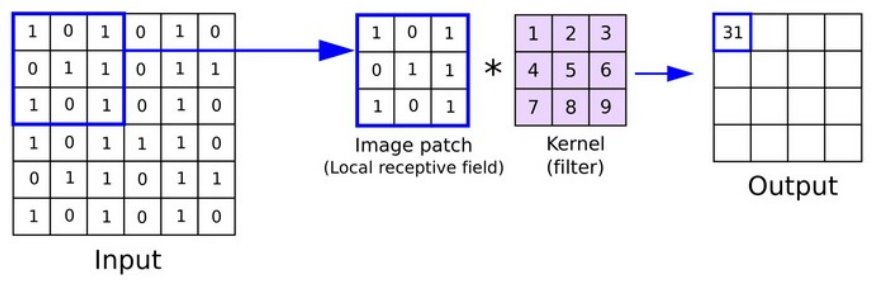
\includegraphics[width=12cm]{Images/convolutional-layer.jpg}
        \caption{Convolutional layer are used to create a feature map}
    \end{figure}

    We can perform the convolutional operation with a certain stride. This is the step size at which the filter moves across the input data. Having a stride different than 1 makes the size of our image to reduce by this factor. Instead, if it is only 1 the dimensionality of the next layer will be N - filter size + 1.

\newpage
    \item Pooling Layer. After the convolutional layer a pooling layer is usually applied to the set of feature maps that we get as the output of the convolutional layer. This pooling layer consists in performing some pooling operation (the most common one of which is max-pooling) to the output of the convolutional layer in order to reduce its size (down-sampling). Pooling helps make the representation become approximately invariant to small translations of the input.

    \begin{figure}[h]
        \centering
        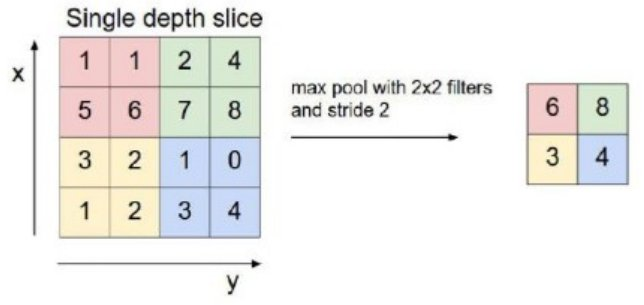
\includegraphics[width=8cm]{Images/max-pooling.jpg}
        \caption{Max pooling}
    \end{figure}
    In pooling we can also specify a certain stride which determines the step size at which the pooling kernel moves across the input data. A stride of k will reduce the image size by a factor of k.

    \item Fully Connected Layer. Usually at the end of the Convolutional Neural Network after a set of convolutional and pooling layers a fully connected layer is implemented. As in FNN this consists in connecting all the input neurons with all the output layer units. An activation function is applied in order to give the output of the Convolutional Neural Network.
    \begin{figure}[h]
        \centering
        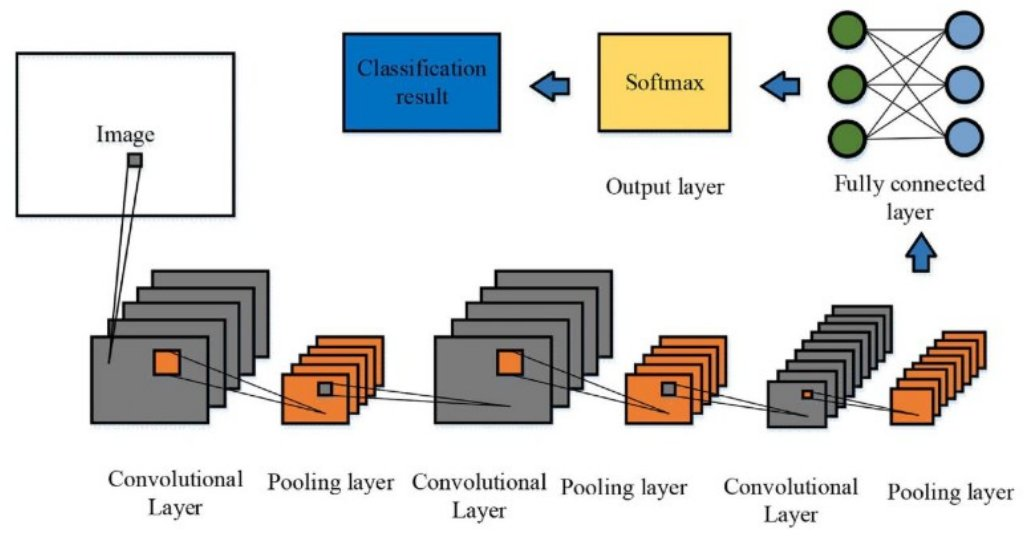
\includegraphics[width=10cm]{Images/cnn.jpg}
        \caption{Convolutional Neural Network Architecture}
    \end{figure}

    Notice that this fully connected layer takes the flattened set of feature maps from the preceding convolutional and pooling layers as input. In this way we will be able to make predictions or classifications based on the features learned by the preceding layers.

    After having the output we will be able to compare the output of our Convolutional Neural Network with the labels and build our loss function. With the loss function then we will perform backpropagation in order to update the parameters. This process is repeated for a number of N epochs.

\end{itemize}

\newpage
\section{Convolution Main Properties}

Convolution leverages two important features: local connectivity and parameter sharing. Let’s review them.

\begin{itemize}
    \item Local Connectivity. Due to the filter kernel being much smaller than the input data we will have only local connectivity. Therefore a point in the output feature map of the convolutional layer is only influenced by a small subset of nearby points in the input data. In a deep Convolutional Neural Network, units in the deeper layers may indirectly interact with a larger portion of the input. This allows the network to efficiently describe more complex interactions of the data by detecting combinations of the features that the previous layer have build.

    \begin{figure}[h]
        \centering
        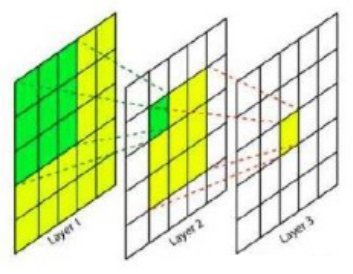
\includegraphics[width=4cm]{Images/local-connectivity.jpg}
        \caption{Local Connectivity}
    \end{figure}

    \item Parameter Sharing. Contrary to traditional Neural Networks in a Convolutional Neural Network each member of the kernel (filter) is used for every position of the input. So, instead of learning a separate set of parameters for every location we learn only one set per filter for every convolutional layer. This makes convolution more efficient than dense matrix multiplication and it also makes our model equivariance to translation (variations in the image data will also produce the same kind of variation in the output data).
    \begin{figure}[h]
        \centering
        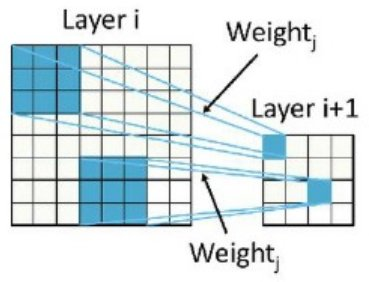
\includegraphics[width=4cm]{Images/parameter-sharing.jpg}
        \caption{Parameter Sharing}
    \end{figure}

\end{itemize}

\newpage
\section{Variants of the Basic Convolution Function}
\subsection{Padding}

One essential feature of any convolutional network implementation is the ability to implicitly zero-pad the input V in order to make it wider. Zero padding the input allows us to control the kernel width and the size of the output independently. This is basically done to not lose information with the pixels around the edges of the image. We have two types of padding: Valid padding and Same padding.

\begin{figure}[h]
    \centering
    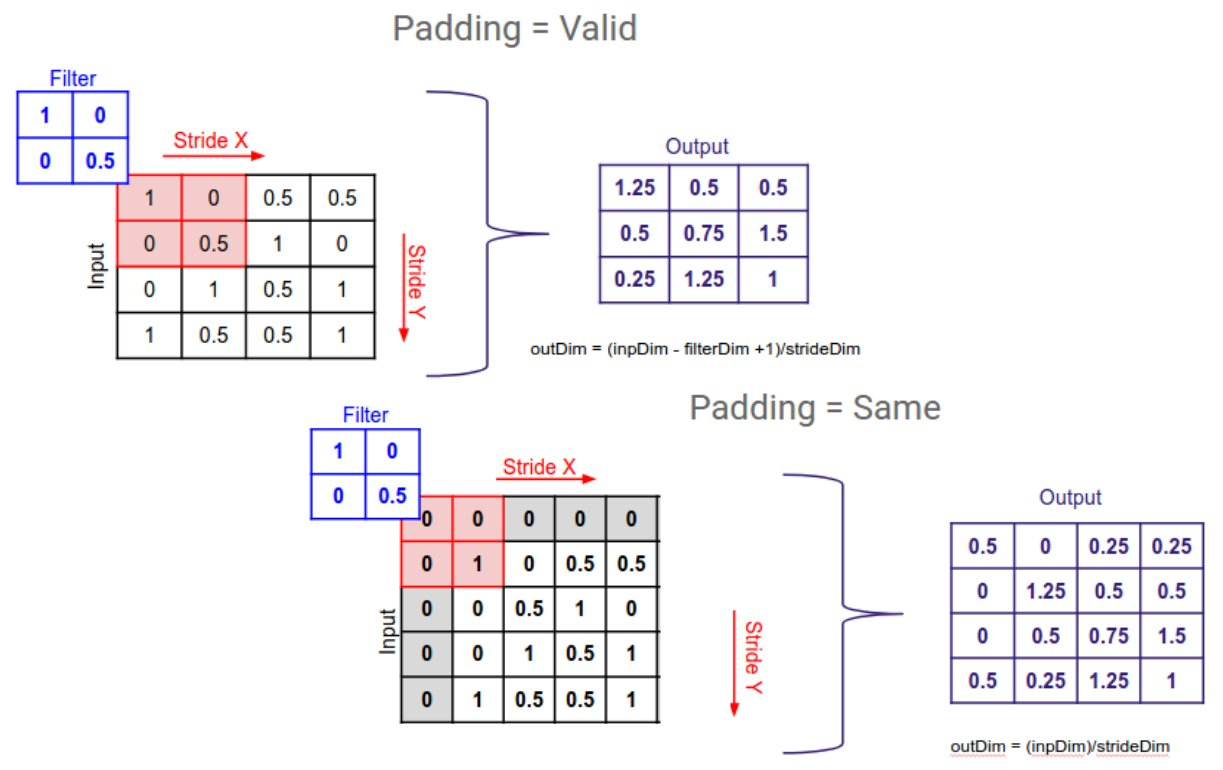
\includegraphics[width=10.5cm]{Images/padding.jpg}
    \caption{Padding}
\end{figure}

\begin{itemize}
    \item Valid padding consists of not applying any padding whatsoever. In this case, the size of the input shrinks at each layer. If the input image has width $m$ and the kernel has width $k$, the output will be of width $m - k + 1$.
    \item Same padding on the other hand consists of adding just enough zeros to keep the size of the output equal to the size of the input. However, the input pixels near the border influence fewer output pixels than the input pixels near the center so it can still make the border pixels somewhat underrepresented in the model.
\end{itemize}

\newpage
\subsection{Multichannel Inputs}

In the context of images, a single-channel image represents gray-scale intensity values, however, images can also have multiple channels, representing the three primary colors known as RGB channels. In this case, the convolutional filters are 3D, adding to the width and height dimensions also the number of channels. During the convolution operation, the filters slide across the input volume, computing element-wise multiplications with the corresponding input values from all channels and summing them to produce the output.

\begin{figure}[h]
    \centering
    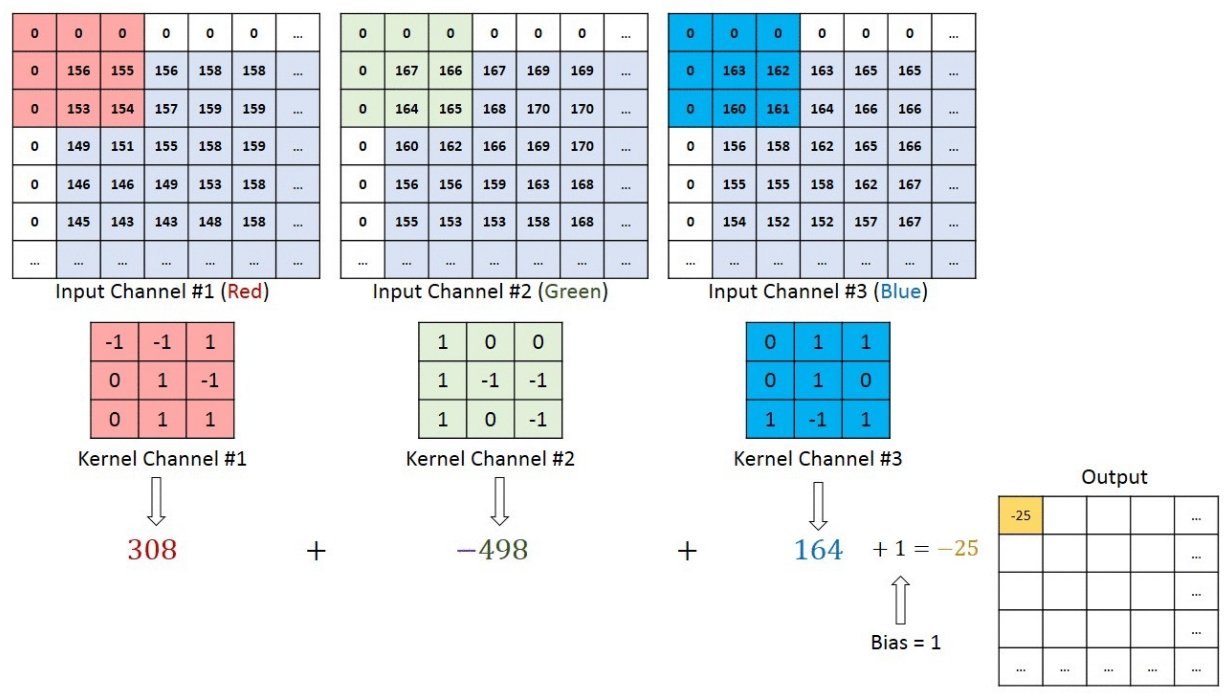
\includegraphics[width=15cm]{Images/rbg-filters.jpg}
    \caption{Multichannel inputs}
\end{figure}


    \chapter{Sequence Modeling: Recurrent and Recursive Networks}

Recurrent Neural Networks are a type of Neural Network architecture that works with sequential data. This is data structured in a sequence where the order holds significance and carries information. Examples: speech and audio data, time series data, textual data, ... 

\noindent Previously we have seen Feedforward Neural Networks and Convolutional Neural Networks architectures. These architectures have what is called a one to one relationships as they both have a fixed size input, a set of hidden layers and finally a single output (or output set). Instead when working with sequential data, we can have:

\begin{itemize}
    \item Many to One Relationships. These are used in sequence classification tasks (e.g. Sentiment classification) which imply having sequential inputs and a single output or output set. 
    \item One to Many Relationships. These architectures are used in sequence generations tasks (e.g. Image Captioning) which is composed of a single input and a sequential output.
    \item Many to many Relationships. These are used in sequence transductions tasks (e.g. Machine translation) which consists of a sequential input and sequential output. In the specific case where we have the same length for both the input and the output we are in an IO-transduction (e.g. Phoneme recognition system).
\end{itemize}

\begin{figure}[h]
    \centering
    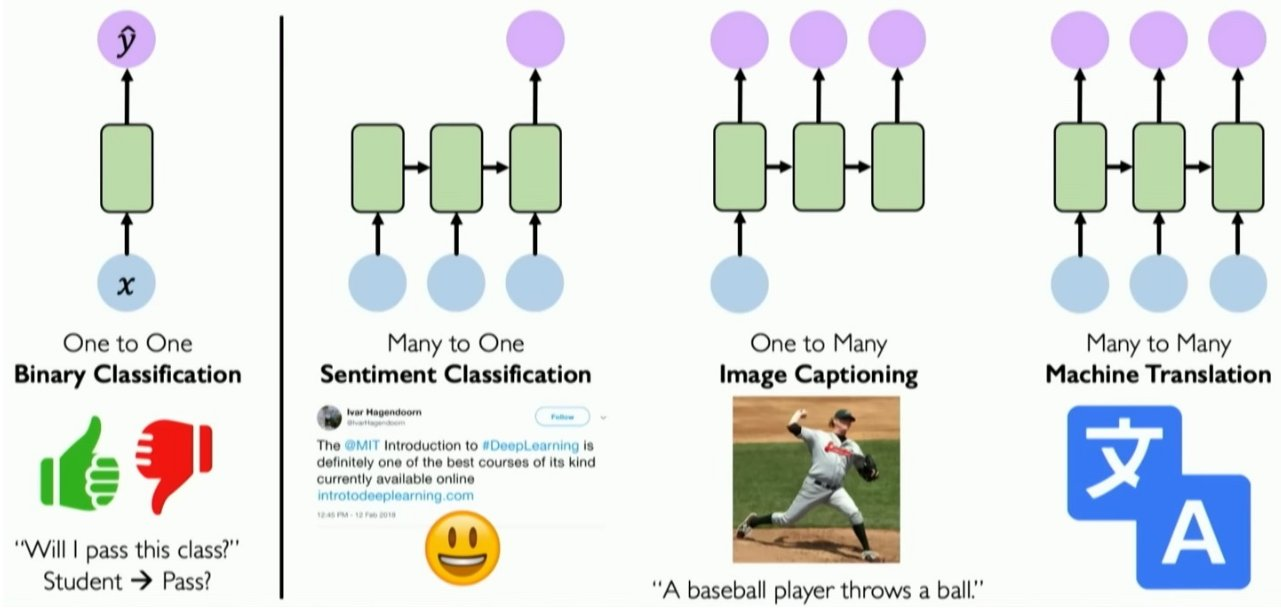
\includegraphics[width=15cm]{Images/sequence-to-sequence.jpg}
    \caption{Sequence to sequence }
    \label{fig:sequence-to-sequence}
\end{figure}

\newpage
\section{Sequential Transduction}

A sequential transduction $T$ refers to the transformation of an input sequence $X = x^{(1)}, ..., x^{(n)}$ into the corresponding output sequence $Y=y^{(1)}, ..., y^{(m)}$ where $n$ and $m$ are the length of the input and output sequences respectively.

\subsection{Memory}

A sequential transduction $T$ has finite memory $k \in N$ if $ \forall ~ x \in X$ and $\forall ~ t, T(x^{(t)})$ only depends on the sequence $ \left ( x^{(t)}, x^{(t-1)}, ..., x^{(t-k)}  \right ) $. Basically this means that its transformation process only requires a bounded and limited amount of information from the input sequence's past elements to produce the output sequence.

\begin{figure}[h]
    \centering
    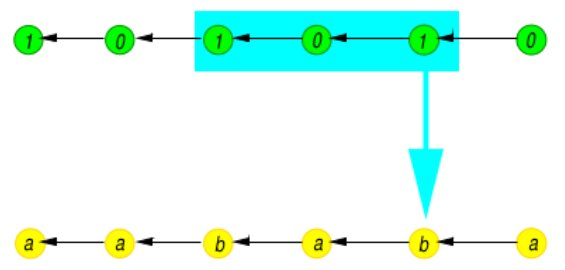
\includegraphics[width=6cm]{Images/transduction-memory.jpg}
    \caption{Transduction Memory}
    \label{fig:transduction-memory}
\end{figure}

\noindent A sequential transduction $T$ is algebraic if it has 0 memory ($k=0$) meaning that its transformation process is solely determined by the input element at the current position $x^{(t)}$ and does not rely on any previous elements in the sequence. An algebraic transduction is memory-less.

\subsection{Causality}

A sequential transduction $T$ is casual if the output at time $t$ does not depend on future inputs (at time $t+1$, $t+2$, ...). In sequential transductions, causality is respected, meaning that the transformation of an element in the output sequence depends only on the elements that have already appeared in the input sequence.

\begin{figure}[h]
    \centering
    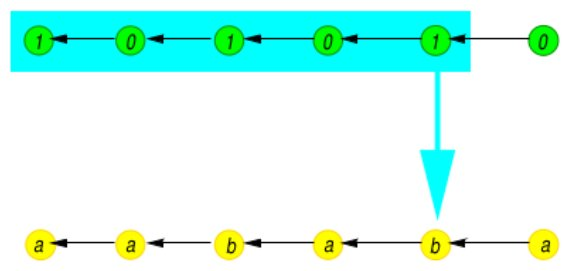
\includegraphics[width=6cm]{Images/causality.jpg}
    \caption{Causality}
    \label{fig:causality}
\end{figure}

\subsection{Stationary}

A sequential transduction $T$ is stationary if the transformation it applies to the input sequence $T(x^{(t)})$ is independent of the position within the sequence. In other words, we will get the same outcome regardless of the value of $t$.

\newpage
\section{Recurrent Neural Network Architecture}

Recurrent Neural Networks are based on the idea of employing recurrent units that maintain hidden states. These states capture information from the current input and the previous hidden state, allowing the network to learn and remember patterns across time steps. The basic Recurrent Neural Network unit takes an input vector $x^{(t)}$ at time step $t$ and a hidden state vector $h^{(t-1)}$ from the previous time step in order to compute the new hidden state $h^{(t)}$:

$$ h^{(t)} = \sigma \left( U x^{(t)} +  W h^{(t-1)} \right ) $$

\noindent where U and W are the weight matrices for the current and previous state. The network returns an output o at a given time-step t:

$$ o^{(t)} = \sigma \left( V h^{(t)} \right) $$

\noindent For every time step the Recurrent Neural Network has only a single hidden layer which maintains a hidden $ h^{(t)}$ at each time step $t$, and this is updated sequentially as the Recurrent Neural Network processes the input sequence.

\noindent To process a sequence of inputs $x^{(t)}$ we apply the basic Recurrent Neural Network unit at each time step t. We can unroll this loop-like diagram in order to represent the Recurrent Neural Network as a computational graph unrolled across time.

\begin{figure}[h]
    \centering
    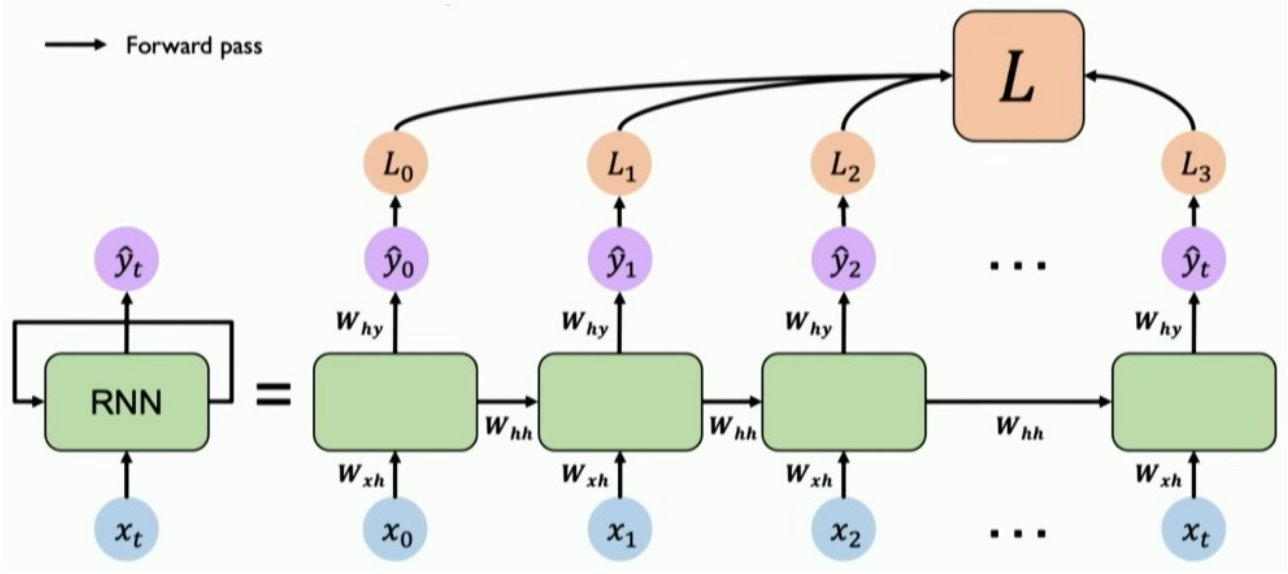
\includegraphics[width=15cm]{Images/rnn.jpg}
    \caption{Recurrent Neural Network Unrolled}
    \label{fig:rnn}
\end{figure}

\newpage
\noindent We can also describe the hidden representation in a Recurrent Neural Network as:

$$ q^{-1} h^{(t)} = h^{(t-1)} $$

Where $q$ is a unitary time delay operator, which means it shifts the hidden state representation $h^{(t)}$ from the current time step $t$ to the next time step $t + 1$. As you can guess $q^{-1}$ does the inverse operation of q. It shifts the hidden state representation $h^{(t)}$ from the current time step $t$ to the previous time step $t - 1$.

\begin{figure}[h]
    \centering
    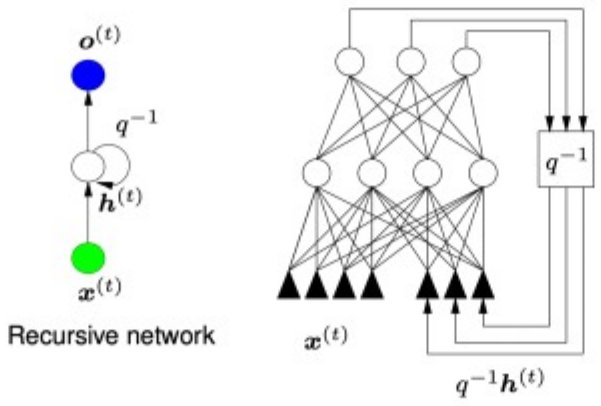
\includegraphics[width=9cm]{Images/rnn-time-delay.jpg}
    \caption{Recurrent Neural Network with time delay representation}
    \label{fig:rnn-time-delay}
\end{figure}

\section{Algorithm}

The overall Recurrent Neural Network algorithm works as follows:

\noindent At the beginning of the sequence processing we initialize the hidden state $h^{(0)}$ to small random values. We will also initialize in the same way the training matrices $U$, $W$ and $V$, and biases $b$ and $c$. We will also set the hyper-parameters which include the learning rate, number of hidden units, activation functions used in the hidden layers, the batch size, ... Now for every time step $ t = 1, ..., T$ we compute the linear transformation of the current input $x^{(t)}$ using the input-to-hidden weights matrix $U$:

$$ U x^{(t)}$$

\noindent This represents the transformed input information at time step $t$. It is often referred to as the pre-activation because it determines how much influence the current input $x^{(t)}$ should have on the new hidden state $h^{(t)}$. Each row of $U$ corresponds to a hidden unit in the Recurrent Neural Network, and each column corresponds to an element in the input at step t $x^{(t)}$. The weights of the matrix control how much each element in the input will contribute.

\noindent Now we compute the linear transformation of the previous hidden state $h^{(t - 1)}$ using the hidden-to-hidden weight matrix $W$.

$$ W h^{(t-1)} $$

\noindent The $W$ matrix determines how information from the previous time step is carried over to the current time step. Each row of $W$ corresponds to a hidden unit, and each column corresponds to a hidden unit from the previous time step.
We can apply an activation function to the combination of both results adding a bias term b to get the hidden state of the actual time step t.

$$ h^{(t)} = \sigma \left( U x^{(t)} + W h^{(t-1)} + b \right) $$

\noindent Finally, compute the output $o^{(t)}$ of the current time-step using the hidden state $h^{(t)}$ and the matrix $V$.

$$ o^{(t)} = \sigma \left(V h^{(t)} + c \right) $$

where the matrix $V$ defines how the information of the hidden state is used to generate the output at each time step. This will be the case if our Recurrent Neural Network is designed for sequence-to-sequence or vector to sequence tasks as an output $o^{(t)}$ will be generated for every time-step in the sequence. The final output is the sequence of all the individual outputs $o^{(t)}$, generated at each time step t:

$$ o = \left[ o^{(1)},  o^{(2)}, ...,  o^{(T)} \right]  $$

\noindent If instead we have a sequence to single output architecture we will get the result $o$ as:

$$ o^{(T)} = \sigma \left(V h^{(T)} + c \right) $$

\noindent By comparing the generated output sequence to the target sequence we can calculate the loss L. 

$$L = - \sum_{t} log (p_{model}) = - \sum_{t} log \left( p \left( y^{(t)} | x^{(1)}, ..., x^{(t)} \right) \right)$$

\noindent which we can use to update the model parameters, by computing the gradients of the loss with respect to them using either Back-Propagation Through Time (BPTT) or Real-Time Recurrent Learning algorithms. This will allow us to update the model parameters using a gradient descent algorithm (e.g. SGD, Adam, etc.) with a learning rate $\eta$. This can be repeated by a number of epochs N in order to improve the network results minimizing the loss.


\section{BPTT vs RTRL}

Backpropagation Through Time and Real-Time Recurrent Learning are two different algorithms used in training Recurrent Neural Networks. They both address the challenge of training networks with temporal dependencies, but they do so in distinct ways.

\subsection{Back-Propagation Through Time}

Back-Propagation Through Time is typically used in a batch learning setting. it involves processing the entire sequence and accumulating the gradients over the entire sequence before performing a weight update. We will start the backward pass from the last time step $t = T$ and work backwards to $t = 1$. So given the loss at each time step $L(t)$ we will start by computing the gradient of the loss with respect to the output matrix $V$.

$$ \frac{\partial L^{(T)}}{\partial V } = \frac{\partial L^{(T)}}{\partial o^{(T)} } \frac{\partial o^{(T)}}{\partial V } $$


\noindent Then we can compute the gradient of the loss with respect to the hidden to hidden state matrix $W$ and the input to hidden state matrix $U$.

$$ \frac{\partial L^{(T)}}{\partial W } =  \frac{\partial L^{(T)}}{\partial o^{(T)} } \frac{\partial o^{(T)}}{\partial W } ~~~~~ \frac{\partial L^{(T)}}{\partial U } =  \frac{\partial L^{(T)}}{\partial o^{(T)} } \frac{\partial o^{(T)}}{\partial U }
$$

\newpage
\noindent In order to get these two values we will need to apply the chain rule:

$$ \frac{\partial o^{(T)}}{\partial W} = \sum_{t'=1}^{T} \frac{\partial o^{(T)}}{\partial h^{(T)}} \frac{\partial h^{(T)}}{\partial h^{(t')}} \frac{\partial h^{(t')}}{\partial W} ~~~~~~~ \frac{\partial o^{(T)}}{\partial U} = \sum_{t'=1}^{T} \frac{\partial o^{(T)}}{\partial h^{(T)}} \frac{\partial h^{(T)}}{\partial h^{(t')}} \frac{\partial h^{(t')}}{\partial U} $$

\noindent Where

$$ \frac{\partial h^{(t)}}{\partial h^{(t')}} = \prod_{j=t'+1}^{t} \frac{\partial h^{(j)}}{\partial h^{(j-1)}}$$

\begin{figure}[h]
\centering     %%% not \center
\subfigure[Backpropagation of gradient W]{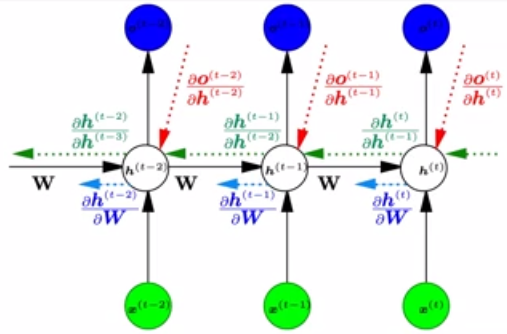
\includegraphics[width=7cm]{Images/bptt-w-matrix.png}}
\subfigure[Backpropagation of gradient U]{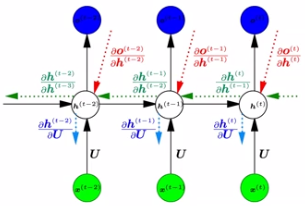
\includegraphics[width=7cm]{Images/bptt-u-matrix.png}}
\end{figure}


\noindent Notice that because Recurrent Neural Networks computations at each time step are dependent on the computations from the previous time step, we will need to propagate the gradients backwards in time, starting from the last time step.

\noindent This is then repeated for every time step. At the end of this process, you will have computed the gradients of the loss with respect to the three weight matrices for each time step $t$. Summing the values for each time step will give us the total gradient values.

$$ \frac{\partial L}{\partial V } = \sum_{t=1}^{T} \frac{\partial L^{(t)}}{\partial V } ~~~~~ \frac{\partial L}{\partial W } = \sum_{t=1}^{T} \frac{\partial L^{(t)}}{\partial W }  ~~~~~ \frac{\partial L}{\partial U } = \sum_{t=1}^{T} \frac{\partial L^{(t)}}{\partial U } $$

\noindent We can use that to update the weight matrices $U$, $V$ and $W$ using an optimization algorithm based on gradient descent.

$$ U \leftarrow U - \eta \frac{\partial L}{\partial U}  ~~~~~ V \leftarrow V - \eta \frac{\partial L}{\partial V} ~~~~~ W \leftarrow W - \eta \frac{\partial L}{\partial W}$$

\newpage
\subsection{Real Time Recurrent Learning}
 
Instead, Real Time Recurrent Learning is designed for online learning, as it updates the gradient at each forward propagation step. This makes this algorithm suitable for real-time applications where updates need to be made continuously every time you receive a new input. Real Time Recurrent Learning directly computes the gradients of the loss with respect to the weights using the exact equations for Recurrent Neural Networks, without unrolling the network.

 Therefore, instead of waiting to compute the whole Loss for the entire sequence and then calculate the gradients by backpropagation, we will be able to compute the gradient in the forward phase. Given a time step $t$ we can consider computing the gradient up to that time step by back-propagating from that time step backwards. Starting at $t=1$ we will be able to compute the gradient at that time step and update the weights. Then we will move forward, and do the same for every time step by remembering that the gradient of the loss up to time $t$ can be computed just by adding the gradient at time $t$ to the previous gradient up to time $t-1$. By doing this from $t=1$ to $t=T$ we will end up computing the same gradient as when performing the Back-Propagation Through Time algorithm.

$$ \frac{\partial L|_t}{\partial V} =  \sum_{t=1}^{t} \frac{\partial L^{(t)}}{\partial o^{(t)} } \frac{\partial o^{(t)}}{\partial V  } = \frac{\partial L|_{t-1}}{\partial V} + \frac{\partial L^{(t)}}{\partial o^{(t)} } \frac{\partial o^{(t)}}{\partial V  }  $$

\noindent In the same way:

$$ \frac{\partial L|_t}{\partial U} =  \sum_{t=1}^{t} \frac{\partial L^{(t)}}{\partial o^{(t)} } \frac{\partial o^{(t)}}{\partial U  } = \frac{\partial L|_{t-1}}{\partial U} + \frac{\partial L^{(t)}}{\partial o^{(t)} } \frac{\partial o^{(t)}}{\partial U  } ~~~~~  \frac{\partial L|_t}{\partial W} =  \sum_{t=1}^{t} \frac{\partial L^{(t)}}{\partial o^{(t)} } \frac{\partial o^{(t)}}{\partial W  } = \frac{\partial L|_{t-1}}{\partial W} + \frac{\partial L^{(t)}}{\partial o^{(t)} } \frac{\partial o^{(t)}}{\partial W  }  $$

\noindent The downside of Real Time Recurrent Learning is that usually the amount of memory and time to compute it is larger than while performing Back-Propagation Through Time. This is why unless you are performing online learning this algorithm is not used so much. 

\begin{table}[h!]
\centering
\begin{tabular}{ p{6cm} p{3cm} p{3cm} } 
\hline\hline
\multirow{2}{*}{Algorithm} & \multicolumn{2}{c}{Complexity}\\ \cline{2-3}\\ & Space & Time \\ \hline

Back-Propagation Through Time & $O(NT)$ & $O(N^{2}T)$ \\ 
Real Time Recurrent Learning & $O(N^{3})$ & $ O(N^{4})$ \\
\hline
\end{tabular}
\end{table}

\noindent As you can see,  Real Time Recurrent Learning will only be more efficient than Back-Propagation Through Time when the number of time steps $T$ is very big. Specifically when $T > N^{2}$ where $N$ is the number of units.

\newpage
\section{Additional Architectural Features for Recurrent Neural Networks}

We can add features to the Vanilla Recurrent Neural Network architecture that make the network behave differently. Let's review some of them:

\subsection{Short-cut Connections}

Short-cut Connections. Shortcut connections, are used to skip some of the connections between the input and the hidden layers, effectively bypassing some of the intermediate layers.

\begin{figure}[h]
    \centering
    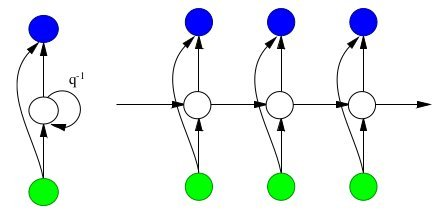
\includegraphics[width=8cm]{Images/short-cut-RNN.jpg}
    \caption{Shortcut in A Recurrent Neural Network}
    \label{fig:shortcut}
\end{figure}

\noindent The output $o^{(t)}$ then will be:

$$ o^{(t)} = \sigma \left(V^{h} h^{(t)} + V^{x} x^{(t)} + c \right) $$

Now both the hidden state $h^{(t)}$ and the input $x^{(t)}$ contribute to the output $o^{(t)}$ (via $V^{h}$ and $V^{x}$ respectively). This means that the network takes both the historical context represented by the hidden state and the current input into account when making predictions.

\subsection{Higher Order States}

Higher order states refer to hidden states that capture dependencies beyond just the immediately preceding time step. In a standard Recurrent Neural Network, the hidden state at a given time step is typically based on the input at that time step and the hidden state at the previous time step. However, higher-order states go beyond this one-step dependency and capture information from further back in the sequence.

\begin{figure}[h]
    \centering
    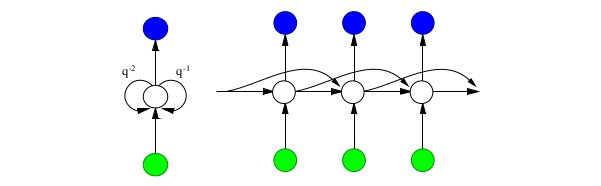
\includegraphics[width=12cm]{Images/higher-order-RNN.jpg}
    \caption{2nd Order State}
    \label{fig:higher-order}
\end{figure}

\noindent The hidden state $h^{(t)}$ then will be:

$$ h^{(t)} = \sigma \left( U x^{(t)} + W^{(1)} h^{(t-1)} + W^{(2)} h^{(t-2)} + b \right) $$

\subsection{Feedback from Output}

Feedback from the output relates to how the network's own predictions at a previous time step can influence the predictions it makes at the current or subsequent time steps. This feedback loop can have a significant impact on the network's behavior and is related to the concept of teacher forcing in training Recurrent Neural Networks. 

\begin{figure}[h]
    \centering
    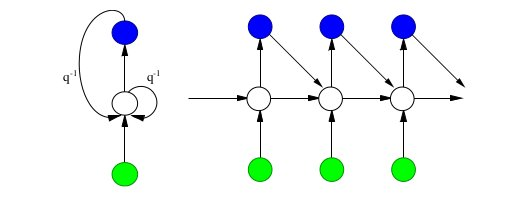
\includegraphics[width=10cm]{Images/output-feedback.jpg}
    \caption{Output Feedback in a RNN architecture}
    \label{fig:output-feedback}
\end{figure}

\noindent This modifies the hidden state in the following way:

$$ h^{(t)} = \sigma \left( U x^{(t)} + W h^{(t-1)} + Z o^{(t - 1)} + b \right) $$

\noindent Feedback from the output can be a useful technique for capturing dependencies and maintaining context.

\subsection{Teacher Forcing}

Teacher forcing is very similar to feedback from the output feature but instead of providing the last step prediction the hidden state takes as input the last step true target. This reduces the accumulation of errors, allowing the network to learn from its mistakes quickly. However, this can lead to exposure bias, where the model struggles to generate sequences independently during inference because it hasn't learned to cope with its own errors.

\begin{figure}[h]
    \centering
    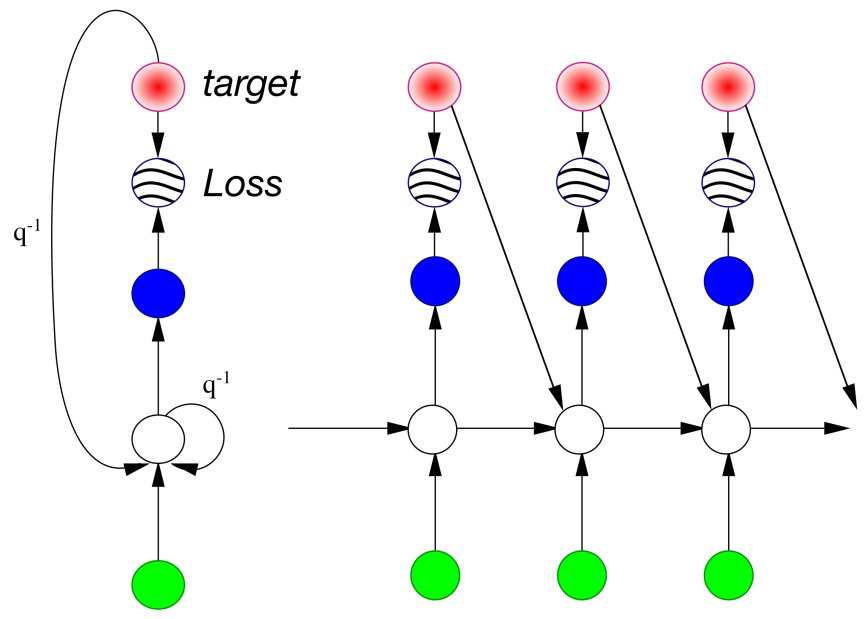
\includegraphics[width=8cm]{Images/teacher-forcing.jpg}
    \caption{Teacher Forcing in a RNN architecture}
    \label{fig:teacher-forcing}
\end{figure}

\noindent Using teacher forcing, the hidden state will be:

$$ h^{(t)} = \sigma \left( U x^{(t)} + W h^{(t-1)} + Z y^{(t - 1)} + b \right) $$

\newpage
\noindent In both feedback from the output and teacher forcing the $Z$ matrix represents a weight matrix that defines the connection between the previous output $o^{(t-1)}$ and the current hidden state $h^{(t)}$. Basically it controls how much influence the previous output has on the current hidden state. As every weight matrix, their values are learned during the training of the Recurrent Neural Network.


\subsection{Bidirectional Recurrent Neural Networks}

When the the sequence is not temporal (or we are processing the data off-line) we can use Bidirectional Recurrent Neural Networks. In this architecture, the output depends both on past and future values of the sequence.

\begin{figure}[h]
    \centering
    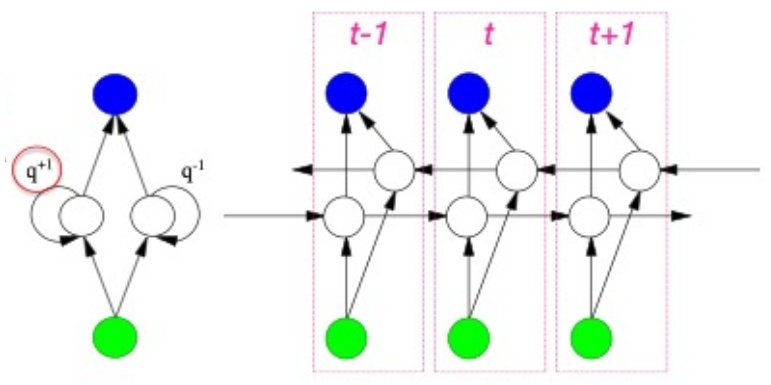
\includegraphics[width=9cm]{Images/bidirectional.jpg}
    \caption{Bidirectional Recurrent Neural Network}
    \label{fig:bidirectional}
\end{figure}

\noindent The output equation for a Bidirectional Recurrent Neural Network  will be:

$$ o^{(t)} = \sigma \left(V^{(p)} {h_p}^{(t)} + V^{(f)} {h_f}^{(t)} + c \right) $$

$$ h_p^{(t)} = \sigma \left( U^{(p)} x^{(t)} + W^{(p)} {h_p}^{(t-1)}  \right)  ~~~~~ h_f^{(t)} = \sigma \left( U^{(f)} x^{(t)} + W^{(f)} {h_f}^{(t+1)}  \right) $$

\noindent where $h_p^{(t)}$ encodes the hidden state for the past history and $h_f^{(t)}$ does the same for the future history.

\noindent All these architectural features (and others...) are orthogonal, meaning that they can be combined together.

\newpage
\section{Encoder-Decoder Sequence-to-Sequence Architectures}

Until now we have consider the Recurrent Neural Networks able to map an input sequence to a fixed-size vector, a fixed-size vector to a sequence and an input sequence to an output sequence of the same length. However, we haven't consider an architecture able to map an input sequence to an output sequence which is not necessarily of the same length. This comes up in many applications, such as speech recognition or machine translation.

The simplest Recurrent Neural Network architecture for mapping a variable-length sequence to another variable-length sequence is called the encoder-decoder or sequence-to-sequence architecture. The idea is very simple. First, an encoder processes an input sequence $X = x^{(1)}, ..., x^{(n_x)}$ and emits a context $C$ which represents a semantic summary of the input sequence. On the other hand, the decoder is conditioned on that fixed-length vector to generate the output sequence $Y = y^{(1)}, ..., y^{(n_y)}$.



\begin{figure}[h]
    \centering
    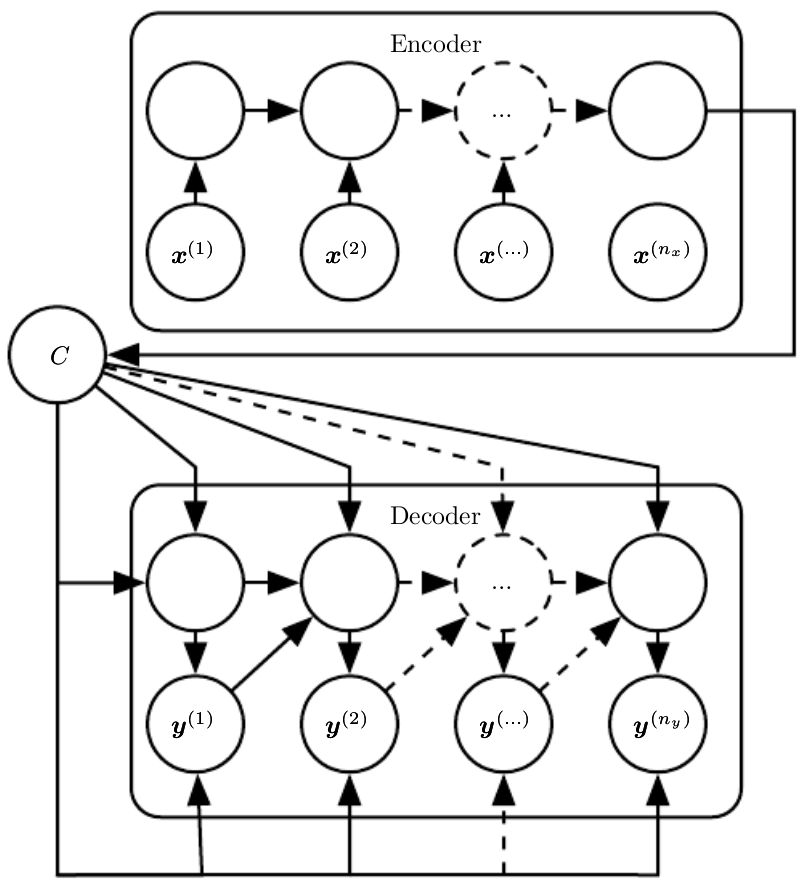
\includegraphics[width=10cm]{Images/encoder-decoder.png}
    \caption{Encoder-Decoder Architecture}
\end{figure}

\noindent In a sequence-to-sequence architecture, the two Recurrent Neural Networks are trained jointly to maximize the average of $\log P \left( y^{(1)}, ..., y^{(n_y)} | x^{(1)}, ..., x^{(n_x)}  \right) $ over all the pairs of $x$ and $y$ sequences in the training set. The last state $h^{(n_x)}$ of the encoder Recurrent Neural Network is typically used as a representation $C$ of the input sequence that is provided as input to the decoder Recurrent Neural Network.

\noindent One clear limitation of this architecture is when the context $C$ output by the encoder Recurrent Neural Network has a dimension that is too small to properly summarize a long sequence. To solve that, alternatives such as using an attention mechanism have found to be successful.

\newpage
\section{The Challenge of Long-Term Dependencies}

When trying to learn long-term dependencies in Recurrent Networks we face a major problem derived from how gradients propagated over many stages tend to either vanish or explode. Moreover, even by assuming that the parameters are stable, the difficulty with long-term dependencies arises from the exponentially smaller weights given to long-term interactions (involving the multiplication of many Jacobians) compared to short-term ones. 

\noindent We can look further by considering that the recurrence relation resembles a matrix multiplication.

$$h^{(t)} = W^{T} h^{(t-1)}$$

\noindent Iterating we get:

$$h^{(t)} = \left(W^{t} \right) ^T   h^{(0)}$$

\noindent If we consider that $W$ admits an eigendecomposition of the form

$$ W = Q \Lambda Q^T $$

\noindent with orthogonal $Q$, the recurrence may be simplified further to

$$ h^{(t)} = Q^T \Lambda^t Q h^{(0)} $$

\noindent The eigenvalues are raised to the power of $t$ causing eigenvalues with magnitude less than one to decay to zero and eigenvalues with magnitude greater than one to explode. Any component of $h^{(0)}$ that is not aligned with the largest eigenvector will eventually be discarded. This problem is particular to recurrent networks.

\noindent In practice, the experiments show that as we increase the span of the dependencies that need to be captured, gradient-based optimization becomes increasingly difficult, with the probability of successful training of a traditional Recurrent Neural Network via Stochastic Gradient Descent rapidly reaching 0 for sequences of only length 10 or 20.

\newpage
\section{Gated Recurrent Unit}

A Gated Recurrent Unit is a Neural Network architecture designed to address some of the limitations of traditional Recurrent Neural Networks. Same as Recurrent Neural Networks at each time step it receives as input the current state $x^{(t)}$ and the hidden state $h^{(t-1)}$ of the previous step and outputs the hidden state $h^{(t)}$ at the current time.

\begin{figure}[h]
    \centering
    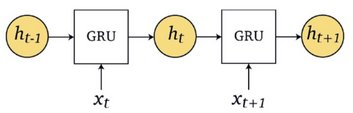
\includegraphics[width=8cm]{Images/gru-schema.jpg}
    \caption{GRU schema}
    \label{fig:gru-schema}
\end{figure}

\noindent The Gated Recurrent Unit addresses the vanishing/exploding gradient problem associated with traditional Recurrent Neural Networks by employing gating mechanisms that carefully control the flow of information through a combination of addition and multiplication operations. These mechanisms consist of the update  gate $z^{(t)}$, reset gate $r^{(t)}$, and the candidate hidden state $\hat{h}^{(t)}$.



\begin{figure}[h]
    \centering
    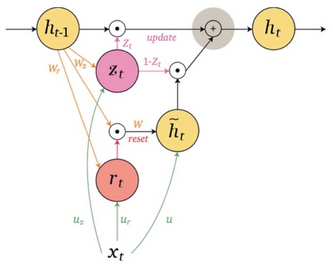
\includegraphics[width=8cm]{Images/gru-architecture.png}
    \caption{Gated Recurrent Unit Architecture}
    \label{fig:gru-architecture}
\end{figure}


\noindent Let's review these gates in more detail:


\subsection{Update Gate}

The update gate $z^{(t)}$ determines how much of the previous hidden state should be retained and is defined as a combination of the current state $x^{(t)}$ and the previous state $h^{(t-1)}$::

$$ z^{(t)} = \sigma \left( W_z h^{(t-1)} + U_z x^{(t)} \right)  $$

\begin{figure}[h]
    \centering
    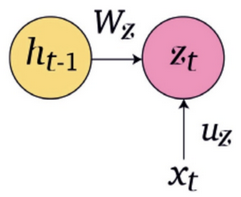
\includegraphics[width=3cm]{Images/update-gate.png}
    \caption{Update Gate}
    \label{fig:update-gate}
\end{figure}

\newpage
\noindent Because we are applying a sigmoid activation function, the output will be between 0 and 1. If the update gate is $z^{(t)} = 0$, then the current hidden state $h^{(t)}$ is the candidate hidden state $h^{(t)} = \hat{h}^{(t)}$. On the other hand, if the update gate is set to $z^{(t)} = 1$, then the output is the previous hidden state $ h^{(t)} = h^{(t-1)}$.

\begin{figure}[h]
\centering     %%% not \center
\subfigure[Update Gate $z^{(t)} = 0$]{\label{fig:update-gate-z0}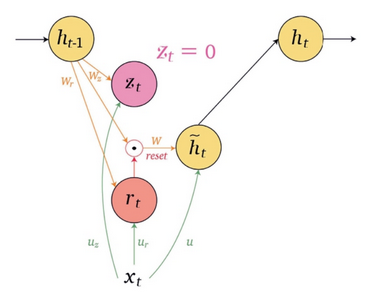
\includegraphics[width=6cm]{Images/update-gate-zt0.png}}
\subfigure[Update Gate $z^{(t)} = 1$]{\label{fig:update-gate-z1}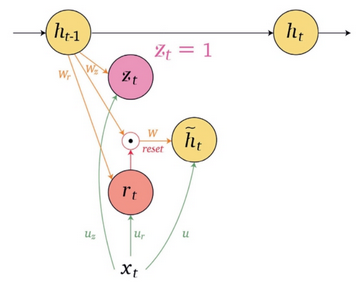
\includegraphics[width=6cm]{Images/update-gate-zt1.png}}
\label{fig:update-gate-zt}
\end{figure}


\noindent Considering that, the hidden state $h^{(t)}$ at time t is a linear interpolation between the previous hidden state $h^{(t-1)}$ and the current candidate $\hat{h}^{(t)}$, which is controlled by the update gate $z^{(t)}$

$$ h^{(t)} = z^{(t)} \odot h^{(t-1)} + (1 - z^{(t)}) \odot \hat{h}^{(t)} $$

\begin{figure}[h]
    \centering
    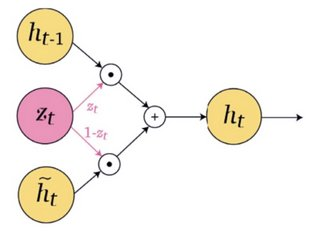
\includegraphics[width=5cm]{Images/gru-update-gate1.jpg}
    \caption{The Update Gate is Used for Interpolation}
    \label{fig:update-gate}
\end{figure}

\subsection{The Candidate}

The candidate hidden state $\hat{h}^{(t)}$ represents the proposed new hidden state that will be considered as an update to the current hidden state and is defined  as combination of the current state $x^{(t)}$ and the previous hidden state $h^{(t-1)}$ and modulated by the reset gate $r^{(t)}$. 

$$ \hat{h}^{(t)} = \phi ( W (r^{(t)} \odot h^{(t-1)}) + U x^{(t)} )  $$

The hyperbolic tangent function applied to the end result ensures that the candidate hidden state values are squashed between the -1 to 1 range, which helps maintain numerical stability in the model.

\begin{figure}[h]
    \centering
    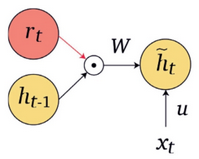
\includegraphics[width=3cm]{Images/candidate.png}
    \caption{Gated Recurrent Unit Candidate }
    \label{fig:candidate}
\end{figure}

\newpage
\subsection{Reset Gate}

The reset gate $r^{(t)}$ is responsible for determining how much of the previous hidden state $h^{(t-1)}$ should be reset or forgotten before computing the candidate hidden state $\hat{h}^{(t)}$.


$$ r^{(t)} = \sigma (W_r h^{(t-1)} + U_r x^{(t)}) $$

\noindent The reset gate is calculated using a sigmoid activation function, which produces values between 0 and 1, similar to the update gate.

\noindent If the reset gate is set to $r^{(t)} = 0$ then the candidate $\hat{h}^{(t)}$ is a function of the current state $x^{(t)}$ such that $\hat{h}^{(t)} = \phi \left( U x^{(t)} \right)$, forgetting the previous hidden state $h^{(t-1)}$. Instead if the reset gate is set to $r^{(t)} = 1$ then the candidate is also a function of the previous state $h^{(t-1)}$.

\begin{figure}[h]
\centering     %%% not \center
\subfigure[Reset Gate $r^{(t)} = 0$]{\label{fig:reset-gate-z0}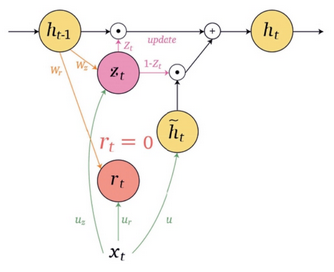
\includegraphics[width=5.5cm]{Images/reset-gate-rt0.png}}
\subfigure[Reset Gate $r^{(t)} = 1$]{\label{fig:reset-gate-z1}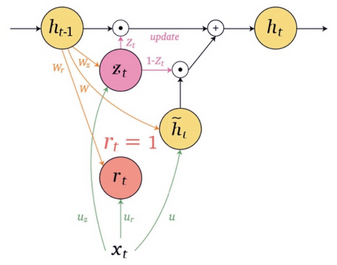
\includegraphics[width=5.5cm]{Images/reset-gate-rt1.png}}
\label{fig:reset-gate-rt}
\end{figure}

\noindent Together with the update gate and candidate hidden state, the reset gate plays a crucial role in determining how the GRU manages its memory and captures relevant information from the sequential data.

\subsection{Special Functionality}

\noindent If $z^{(t)} = 0$ and $r^{(t)} = 0$ then the hidden state is only dependent on the current state \linebreak $h^{(t)} = \phi \left( U x^{(t)} \right)$, forgetting the previous hidden state $h^{(t-1)}$.

\begin{figure}[h]
    \centering
    \includegraphics[width=5cm]{Images/GRUr0z0.png}
    \caption{Gated Recurrent Unit with $r^{(t)} = 0$ and $z^{(t)} = 0$}
    \label{fig:gru-r0-z0}
\end{figure}

\newpage
\noindent Instead if $z^{(t)} = 0$ and $r^{(t)} = 1$ the Gated Recurrent Unit is reduced to a vanilla Recurrent Neural Network such that $h^{(t)} = \hat{h}^{(t)} = \phi \left( W h^{(t-1)} + U x^{(t)} \right)$

\begin{figure}[h]
    \centering
    \includegraphics[width=5cm]{Images/GRUr1z0.png}
    \caption{Gated Recurrent Unit with $r^{(t)} = 1$ and $z^{(t)} = 0$}
    \label{fig:gru-r1-z0}
\end{figure}

\noindent Therefore, the careful management of information through these gates allows to avoid the vanishing gradient problem by learning when to update their memory and when to forget, making them more effective at capturing long-range dependencies in sequential data than vanilla Recurrent Neural Networks. 


\section{Long Short Term Memory (LSTM)}

Long Short-Term Memory is another specialized type of Recurrent Neural Network architecture specifically designed to address the vanishing/exploding gradient problem associated with Recurrent Neural Networks. They achieve this by incorporating gating mechanisms that control the flow of information. These gating mechanisms include the input gate $i^{(t)}$, the forget gate $f^{(t)}$, the output gate $o^{(t)}$ and the memory gate $c^{(t)}$. Additionally, a candidate memory $\hat{c}^{(t)}$ is also introduced.

\begin{figure}[h]
    \centering
    \includegraphics[width=7cm]{Images/lstm-architecture.png}
    \caption{Long Short Term Memory Architecture}
    \label{fig:lstm-architecture}
\end{figure}


\noindent At each time step, it receives as input the current state $x^{(t)}$, the hidden state $h^{(t-1)}$ and a memory cell $c^{(t-1)}$ of the previous time step, and outputs the hidden state $h^{(t)}$ and memory cell $c^{(t)}$ at time t. The memory cells propagate information from the previous state to the next, whereas the hidden states determine the way in which that information is propagated. 

\begin{figure}[h]
    \centering
    \includegraphics[width=6cm]{Images/lstm-sequential.png}
    \caption{Long Short Term Memory}
    \label{fig:lstm-seq}
\end{figure}

\subsection{The Forget Gate}

The forget gate $f^{(t)}$ is responsible for determining how much information from the previous cell state $c^{(t-1)}$ should be forgotten or retained when processing a new input at time step $t$ and is implemented as a combination of the current state $x^{(t)}$ and the previous state $h^{(t-1)}$:

$$ f^{(t)} = \sigma \left( W_f h^{(t-1)} + U_f x^{(t)}   \right) $$

\begin{figure}[h]
    \centering
    \includegraphics[width=3cm]{Images/lstm-forget-gate.png}
    \caption{Long Short Term Memory forget gate}
    \label{fig:lstm-forget-gate}
\end{figure}

\noindent The forget gate applies a sigmoid activation function to its output to produce values between 0 and 1, with 0 indicating complete forget of the previous memory cell $c^{(t-1)}$ and 1 indicating complete retention.



\begin{figure}[h]
    \centering
    \includegraphics[width=8cm]{Images/lstm-forget-gate-f0.png}
    \caption{Long Short Term Memory forget gate for $f^{(t)} = 0$}
    \label{fig:lstm-forget-gate-f0}
\end{figure}

\subsection{Input Gate}

The input gate $i^{(t)}$ is responsible for determining how much new information should be added to the cell state $c^{(t)}$ at time step $t$ based on the current input $x^{(t)}$ and the previous hidden state $h^{(t-1)}$. 

$$ i^{(t)} = \sigma \left( W_i h^{(t-1)} + U_i x^{(t)} \right) $$

\begin{figure}[h]
    \centering
    \includegraphics[width=3cm]{Images/lstm-input-gate.png}
    \caption{Long Short Term Memory input gate}
    \label{fig:lstm-input-gate}
\end{figure}

\newpage
\noindent The input gate is implemented using a sigmoid activation function to produce values between 0 and 1. Values close to 0 in the input gate prevent new information from being added, while values close to 1 allow new information to be fully integrated into the cell state. This mechanism enables to selectively update and maintain information in the internal memory, making them effective at capturing both short-term and long-term dependencies in sequential data.

\begin{figure}[h]
    \centering
    \includegraphics[width=8cm]{Images/lstm-input-gate-i0.png}
    \caption{Long Short Term Memory input gate for $i^{(t)} = 0$}
    \label{fig:lstm-input-gate-i0}
\end{figure}

\subsection{Memory Gate}

The memory cell state $c^{(t)}$ represents the internal memory of the LSTM and is designed to store and carry information over long sequences. It is updated at each time step based on the previous memory cell state $c^{(t-1)}$ and the candidate memory cell $\hat{c}^{(t)}$ at the current time step and controlled by both the input gate $i^{(t)}$ and forget gate $f^{(t)}$.

$$ c^{(t)} = f^{(t)} c^{(t-1)} + i^{(t)} \hat{c}^{(t)}$$

\begin{figure}[h]
    \centering
    \includegraphics[width=4cm]{Images/lstm-memory-gate.png}
    \caption{Long Short Term Memory memory gate}
    \label{fig:lstm-memory-gate}
\end{figure}

\noindent Notice how if the forget gate $f^{(t)}$ is close to 0 the memory cell at time $t$ will ignore the information given by the previous time step. Meanwhile if the input gate $i^{(t)}$ is close to 0 the memory cell at time $t$ will ignore the information given by the new information from the candidate memory cell state. 

\newpage
\subsection{Candidate Memory}

The candidate memory cell state $\hat{c}^{(t)}$ represents the proposed new information that can be added to the memory cell state $c^{(t)}$ at the current time step $t$. It is computed based on the current input $x^{(t)}$ and the previous hidden state $h^{(t-1)}$.

$$ \hat{c}^{(t)} = \phi \left( W h^{(t-1)} + U x^{(t)} \right) $$

\begin{figure}[h]
    \centering
    \includegraphics[width=3cm]{Images/lstm-candidate-memory.png}
    \caption{Long Short Term Memory Candidate Memory}
    \label{fig:lstm-candidate-memory}
\end{figure}

\noindent The hyperbolic tangent function ensures that the values are squashed to the range between -1 and 1, making the proposed information numerically stable. 

\subsection{Output Gate}

The output gate $o^{(t)}$ is responsible for determining how much of the updated memory cell state $c^{(t)}$ should be used to produce the output at the current time step. The output gate takes the current input $x^{(t)}$ and the previous hidden state $h^{(t-1)}$ as inputs and is implemented using a sigmoid activation function to produce values between 0 and 1. Values close to 0 in the output gate prevent information from the memory cell state from affecting the output, while values close to 1 allow the memory cell state to strongly influence the output.

$$ o^{(t)} = \sigma \left( W_o h^{(t-1)} + U_o x^{(t)}     \right)   $$

\begin{figure}[h]
    \centering
    \includegraphics[width=3cm]{Images/lstm-output-gate.png}
    \caption{Long Short Term Memory output gate}
    \label{fig:lstm-output-gate}
\end{figure}

\noindent Where the hidden state $h^{(t)}$ represents the output of the LSTM at each time step. Basically, it represents the information that the LSTM has chosen to propagate to the next time step, considering both the memory cell state and the importance assigned to it by the output gate.

$$ h^{(t)} = o^{(t)} \phi \left( c^{(t)}  \right)$$

\subsection{Peephole Connections}

Peephole connections are a modification to the standard Long Short-Term Memory architecture. These connections allow the gates of the LSTM to have direct access to the previous cell state $c^{(t-1)}$ in addition to the current input $x^{(t)}$ and hidden state $x^{(t)}$. This additional information can improve the ability to control information flow. 

\newpage
\noindent The standard LSTM gates input gate $i^{(t)}$, forget gate $f^{(t)}$, and output gate $o^{(t)}$ are computed without considering the previous cell state. With peephole connections, these gates are modified to include direct access to $c^{(t-1)}$.

forget gate: $ f^{(t)} = \sigma \left( W_f h^{(t-1)} + P_f c^{(t-1)} + U_f x^{(t)} \right)$

input gate: $ i^{(t)} = \sigma \left( W_i h^{(t-1)} + P_i c^{(t-1)} + U_i x^{(t)} \right)$

output gate: $ o^{(t)} = \sigma \left( W_o h^{(t-1)} + P_o c^{(t-1)} + U_o x^{(t)} \right)$

\begin{figure}[h]
    \centering
    \includegraphics[width=6.5cm]{Images/lstm-peepholes.png}
    \caption{Long Short Term Memory with peepholes}
    \label{fig:lstm-peephole}
\end{figure}

\noindent Therefore, Long Short Term-Memory networks are effective in mitigating the vanishing and exploding gradient problems by incorporating gating mechanisms, careful activation functions, and controlled information flow. These mechanisms allow to learn and capture long-range dependencies in sequential data and enable the training of deep networks with more stability and better gradient flow. 


\subsection{Gated Recurrent Unit vs Long Short Term Memory}

\noindent Comparing the interpolation of the new candidate in the Gated Recurrent Unit with the interpolation of the new memory cell in the Long Short Term Memory shows that the update gate $z^{(t)}$ controls the amount of the new candidate to pass in the Gated Recurrent Unit, whereas the input gate controls the amount of the new candidate memory to pass in the Long Short Term Memory. Interpolation in the Gated Recurrent Unit is controlled by a single parameter $z^{(t)}$, whereas in the LSTM interpolation is controlled by two separate parameters $i^{(t)}$ and $f^{(t)}$.

\begin{figure}[h]
\centering     %%% not \center
\subfigure[Gated Recurrent Unit candidate interpolation]{\label{fig:gru-candidate-interpolation}\includegraphics[width=7cm]{Images/gru-candidate-interpolation.png}}
\subfigure[Long Short Term Memory candidate interpolation]{\label{fig:lstm-candidate-interpolation}\includegraphics[width=7cm]{Images/lstm-candidate-interpolation.png}}
\label{fig:lstm-gru-interpolation}
\end{figure}

\newpage
\noindent Comparing the Gated Recurrent Unit reset gate controlling the candidate hidden state with the Long Short Term Memory input gate controlling the candidate memory cell shows the modulation of the candidate in both units.

\begin{figure}[h]
\centering     %%% not \center
\subfigure[Gated Recurrent Unit candidate]{\label{fig:gru-candidate-interpolation}\includegraphics[width=7cm]{Images/gru-candidate.png}}
\subfigure[Long Short Term Memory candidate]{\label{fig:lstm-candidate-interpolation}\includegraphics[width=7cm]{Images/lstm-candidate.png}}
\label{fig:lstm-gru-candidate}
\end{figure}

\noindent Both GRUs and LSTMs address the vanishing gradient problem and excel in sequential data tasks, LSTMs offer more advanced memory management and fine-grained control over information flow. The choice between the two depends on the specific requirements of the task, available data, and computational resources. GRUs are a more lightweight option for many applications, while LSTMs are often preferred when complex, long-range dependencies need to be modeled.


\section{Reservoir Computing Networks}

Reservoir Computing Networks offer an alternative architectural approach to mitigate the vanishing or exploding gradient problem commonly encountered in Recurrent Neural Networks. In a standard RNN, the recurrent weights linking the previous hidden state $h^{(t-1)}$ to the current state $h^{(t)}$, as well as the input weights connecting the input $x^{(t)}$ to $h^{(t)}$, can be challenging to learn effectively. Reservoir Computing Networks address this by introducing a reservoir of $N$ units with fixed, randomly initialized connections. The weight matrices governing connections between these hidden units, as well as those between the hidden units and the input, remain unaltered. This design choice is made to ensure that the recurrent hidden units are able to capture the temporal dependencies of past inputs, while only the output weights are subject to learning.

\begin{figure}[h!]
    \centering
    \includegraphics[width=10cm]{Images/reservoir-network.png}
    \caption{Reservoir Network}
\end{figure}


\noindent The distinctive feature of Reservoir Computing Networks lies in their introduction of a reservoir, a dynamic layer composed of $N$ internal units. This reservoir is characterized by fixed, randomly initialized connections, both within the reservoir and between the reservoir and the input layer. These fixed connections create a dynamic system with a rich state space, allowing the reservoir to naturally capture and propagate information from past inputs to the present state. This is achieved by leveraging the Echo State Property, which encourages the reservoir's internal dynamics to quickly forget initial conditions and be primarily influenced by current inputs. 

\noindent In order to implement the reservoir computing network we need to have an internal memory for the internal units. In Echo State Machines the idea is to have as internal units standard recurrent neurons plus some units working as leaky integrators. This ones are defined by the following formula:

$$ h^{(t)} = (1 - a)h^{(t-1)} + \sigma \left( U x^{(t)} + W h^{(t-1)} \right) $$

where $a$ is the decay rate and is used to control how much of the memory from the previous time step is take into account. This is used in order to be able to keep long term dependencies. For $a=1$ this gives us the equation of the standard recurrent unit. Adding leaky integrators makes the reservoir to remember information from the past. In these type of reservoir network, reservoir's state echoes relevant information from the past inputs, contributing to its ability to capture temporal dependencies. 


\noindent In order to produce a rich set of dynamics, the reservoir should:
\begin{itemize}
    \item Be big. From hundreds to thousands of units.
    \item Be sparse and randomly connected. The number of connections should be low compared to the number of possible connections and those connections should follow a uniform distribution. Keep in mind that the input and output matrices should be dense in order to not lose information from the input or to the output.
    \item Satisfy the echo state property. The effect of the current state $h^{(t)}$ and the current input $x^{(t)}$ on a future state $h^{(t + \tau)}$ should vanish gradually as time passes $\tau \rightarrow \inf$. This basically means that the spectral-radius is $\rho(W) < 1$. The spectral-radius of a matrix is the maximum eigenvalue. This is done so the memory does not saturate. Even if the architecture is designed to learn long term dependencies there should be a way to forget part of them as the iterations go by.
\end{itemize}

\noindent Finally, in Reservoir Computing Networks, the learning process is focused on adapting the weights connecting the reservoir to the output layer. Only these output weights are subject to learning. Indeed the output is computed then as a simple linear combination of the input-excited reservoir which makes it a fast training. By confining the learning process to the output layer, the complexity of training is significantly reduced compared to traditional Recurrent Neural Networks.
















    \chapter{Graph Convolutional Networks}

Instead of working with regular grids like image data we can also work with graphs that can be seen as a sort of irregular grids. Graphs differentiate from images and 1d grids that they don't posses a pre-defined order. The nodes of a graph don't have a strictly relative position between one to another. Instead, they are defined by their connections between them. Contrary to images and sequences where all nodes have the same number of neighbors, the number of edges that each node has may be different.

\noindent Graphs can be of different kinds depending on the constrains we impose to them:

\begin{itemize}
    \item Undirected Graphs. Graphs in which edges have no orientation, meaning that they connect two vertices without any indication of direction.
    \item Directed Graphs. Graphs in which each edge is directed from one vertex to another, indicating a one-way relationship between vertices.
    \item Trees. A tree is a connected acyclic graph where any pair of nodes is connected by exactly one path. The top node is known as root, while the peripheral nodes are known as leaves.
\end{itemize}

\begin{figure}[h]
    \centering
    \includegraphics[width=9cm]{Images/types-graphs.png}
    \caption{Different types of graphs}
\end{figure}

\noindent Regression or classification problems with graphs basically consist of given a dataset composed by $N$ pairs $\left ( G_i, y_i \right)$ with $i = (1, ..., N)$ where $N$ is the number of graphs in the dataset, $G_i$ is one graph and $y_i$ is the target/label associated with that graph, the goal is that given an unseen graph $G$ to predict the correct target/label. Each graph $G$ will also have $n_j$ vertices and a vector of attributes $d$ associated to each node.

\newpage

\noindent Graphs are represented with an adjacency matrix $A$. That is a $N \times N$ matrix such that $A_{ij}=1$ if there is an edge between nodes i and j, and $A_{ij} = 0$ otherwise. For an undirected and unweighted network2 the adjacency matrix is binary and symmetric $A_{ij}= A_{ji}$ while this is not the case of a directed graph. In the case of an undirected weighted network the adjacency matrix is not binary $A_{ij}= W_{ij}$ if there is an edge between nodes $i$ and $j$ with weight $w_{ij}$ and $A_{ij}=0$ otherwise. Usually, the adjacency matrix of a weighted network is indicated by $W$, to distinguish it from its binary counterpart $A$ where the network structure is the same but weights are neglected.

\begin{figure}[h]
    \centering
    \includegraphics[width=12cm]{Images/adjacency-matrices.png}
    \caption{Different types of adjacency matrices}
\end{figure}







\section{Why is Complicated to Learn with Graphs}

A major problem when working with graphs is that many simple operations that are efficient in other data structures, are computationally very expensive when using graphs. For example just to see if two graphs are isomorphic between each other (if they are the same) or if one graph is a subgraph of another graph is expensive. This is important as when performing learning tasks we use the data of the training set to build our model and then when given a test sample we try to predict the output considering similar data that the model has seen in training. Basically, we exploit the similarities between training and test data. When working with graphs we will not be able to that due to the time complexity of performing these tasks.

\newpage

\section{Micheli Model}

One of the first models proposed to adapt Convolutional Neural Networks to graphs was done by professor Micheli. In this architecture, every node in each layer will model a node in the graph. As a result the network has the same structure as the graph.

\begin{figure}[h]
    \centering
    \includegraphics[width=12cm]{Images/nn4g-micheli.png}
    \caption{Architecture of a Neural Network for Graphs proposed by Micheli}
\end{figure}


\noindent A convolution operation is performed in each layer of the network where each convolution takes as input the representation of all previous layers. As in Convolutional Neural Networks the representation computed at a certain layer for a node depends on the same node and its neighbors in the previous layer.

\noindent The representation learned for a node after layer $i$ will be:

$$ h_v^{i} = \sigma \left( \Bar{W}^{i} x_v + W_i \sum_{u \in N(v)} h_{u}^{i-1} \right) $$

\noindent An equivalent matrix formulation:

$$ H^{i} =   \sigma \left(     (\overline{W})^{i} X + W^{i} A H  \right) $$

\noindent Micheli's Graph Neural Network was driven by intuition considering how a Convolutional Neural Network works. Interestingly, we can arrive to a similar formulation following a more formal approach on how to define a convolution operation in a graph.

\newpage
\section{Graph Convolutional Neural Networks}

To extend Convolutional Neural Networks to graphs we will need to exploit the convolution theorem. In the time domain, convolution is an operation that combines two signals to produce a third signal. Mathematically, if we have two signals $f(t)$ and $g(t)$, their convolution $h(t)$ is given by:

$$ h(t) = \int_{-\infty}^{\infty} f(\tau) g(t - \tau) d\tau  $$

which is also represented as $h(t) = f(t)*g(t)$

\noindent In the frequency domain, signals are often represented using their Fourier transforms. The convolution theorem states that the Fourier transform of the convolution of two signals in one domain is equal to the pointwise multiplication of their Fourier transforms. 

$$ F\{f*g\} = F\{f\} \odot F\{g\} $$

\noindent For graphs the Laplacian operator is defined as:

$$  L = I_n - D^{-\frac{1}{2}} A D^{-\frac{1}{2}}$$

\noindent where $A$ is the adjacency matrix and $D$ is a diagonal matrix whose elements represent the degree of each node.

\noindent If the graph is undirected the adjacency matrix is symmetric. Since we can always compute the eigendecomposition in symmetric matrices, we can decompose $L$ as:

$$L = U  \Lambda U^T $$

where $\Lambda$ is a diagonal matrix whose elements are the eigenvalues of the Laplacian matrix and and $U$ is the Fourier basis of the graph.

\noindent Therefore, given a spatial signal $x$, the graph Fourier transform is $\Hat{x} = U^T x$ and the inverse Fourier transform is $x= U \Hat{x}$. Where the graph transform takes you from the graph domain to the spectral domain and the inverse viceversa. By doing this we are able to compute the convolution.

\noindent The convolution between a parametric filter $f_{\theta}$ and a signal $x$ will be defined as:

$$ y = f_{\theta} * x = U \left( \left( U^T f_{\theta} \right) \odot \left( U^T x \right)   \right) $$

where in the frequency domain the convolution is the element-wise multiplication of the Fourier transform of two signals. Since we want the result back to the node domain we apply the inverse Fourier transform $U$.

\noindent Since we don't know how to define the filter in the graph domain, we will work with the filter in the spectral domain $ \hat{f}_{\theta}$ that can be computed as $\hat{f}_{\theta} = U^T f_{\theta}$. Now if we substitute $ f_{\theta}$ in the previous equation we get:

$$ y = f_{\theta} * x = U \left(  \hat{f}_{\theta} \odot \left( U^T x \right)   \right) $$

\noindent We can convert $f_{\theta}$ that is a vector to a diagonal matrix. Doing this we are exploiting the relationship $a \odot b = Ab$ and we will be able to write the convolution operator as:

$$ y = f_{\theta} * x = U \hat{F}_{\theta} U^T x  $$

\newpage
\noindent The filter then can be defined as a polynomial parametric filter using the eigenvalues of the Laplacian matrix:

$$ \hat{F}_{\theta} = \sum_{k=0}^{K} \theta_k \Lambda^K  $$

where $k$ defines the receptive field of the filter.

\noindent Substituting:

$$ y = f_{\theta} * x = U \hat{F}_{\theta} U^T x = \sum_{k=0}^{K} \theta_k U \Lambda^K U^T x = \sum_{k=0}^{K} \theta_k L^k x$$

\noindent By defining the convolution in this way we can compute the convolution directly in the graph domain. Moreover since the Laplacian provides information about random walks in each node we can interpret these filters as encoding random walks in the graph. 


    \chapter{Transformers}

Most competitive neural sequence transduction models have an encoder-decoder structure. The encoder maps an input sequence of symbol representations $x_1, ..., x_n$ (words) to a sequence of continuous representation $ z = z_1, ..., z_n$ (numbers). Given $z$, the decoder then generates an output sequence $y_1, ..., y_m$ of symbols one element at a time. At each step the model is auto-regressive, taking into account the previously generated symbols as additional input when generating the next.

The Transformer follows this overall architecture using stacked self-attention and point-wise, fully connected layers for both the encoder and decoder. Transformers have the advantage over other encoder-decoder based models like LSTM or GRU that they do not use sequential processing and hence they can take advantage of parallel processing and the power of GPUs.

\begin{figure}[h]
    \centering
    \includegraphics[width=6cm]{Images/trasnformer.jpg}
    \caption{Transformer architecture}
    \label{fig:transformer}
\end{figure}

\noindent Let’s see now the overall transformer architecture in detail which was designed for machine translation:

\newpage
\section{Encoder}

The encoder starts by taking an input sequence of symbol representations $x_1 , ... , x_n$ (words) and transforming them by means of a word embedding process. Basically, this consists in taking the input set of words and encode them as numerical vectors in a way that similar words should have similar representation vectors.

Since the model contains no recurrence (that performs operations in a sequential order) we must add information about the relative or absolute positioning of the words in some way. For this reason we will perform a positional encoding operation to the embedding vectors resulting in an additional positional encoding vector. The result will give us the pre-processed data which will be done only once.

\noindent Now let’s talk about the self-attention mechanism that transformers rely on. Self-attention mechanism is designed to capture relationships between different words in a sequence of text.

Self-attention works first by creating three different copies of the input vector embedding. These three vectors are multiplied by three different weight matrices $W^Q$ , $W^K$ and $W^V$ which weights will be learned during the training process. The result of it will be three different matrices called query $Q= X W^Q$ ,keys $K= X W^K$ and values $V = X W^V$.

\noindent We can use these three matrices to calculate self-attention with the following formula

$$ Attention(Q, K, V) = softmax \left( \frac{Q K^T}{\sqrt{d_k}} \right) V $$

This returns a matrix where each row captures the information from the entire sequence with respect to a single word in the sentence. The importance of each word is weighted according to its attention score.

\noindent Instead of performing a single attention calculation between the query (Q), value (V) and key (K) matrices for a given sequence, the Transformer model employs a multi-head attention mechanism. In multi-head attention, the attention process is carried out multiple times in parallel, with each instance focusing on different learned projections of the query, key, and value vectors. This approach allows the model to capture different types of relationships and patterns in the data simultaneously.

\begin{figure}[h]
    \centering
    \includegraphics[width=6cm]{Images/self-attention.jpg}
    \caption{Multi-head attention architecture}
\end{figure}

\noindent The attention block is followed by an add and normalization layer. In this layer we first calculate the sum of the output vector of attention block (that we just calculated) and the input embedding vector. The outcome is then subjected to layer normalization (for stable training and better convergence) and passed to the Feed-forward Neural Network for further processing. The purpose of the Feed-forward Neural Network is to process the outcome of one attention layer to better feed the input of the next attention layer.

\newpage
\noindent After the Feed-forward Neural Network there is another add and norm layer that operates in the same way of the one we just described. With this ends the encoder architecture overview. Remember though that the transformer architecture stacks several encoder blocks in top of each other. In the original paper this number was 6.

\begin{figure}[h]
    \centering
    \includegraphics[width=8cm]{Images/encoder.jpg}
    \caption{Encoder architecture}
\end{figure}


\section{Decoder}

Depending if we are performing training or testing the decoder will work in a different way. In training we are fine-tunning the parameters of our model while in testing we will be using the model to actually translate sentences.

\noindent When working in the test mode, we first feed the sentence in one language (e.g English) into the encoder. After the encoder has process the entire sentence this will produce an output which we will feed to the decoder. Based on this output and in previously translated words the decoder chooses the word that is most likely the correct translation (if it is the first word of the sentence a start of the sentence token will be feed instead). This is repeated for every word in the sentence until our decoder decides that the most probable output will be the end of the sentence token. As you could see the encoder uses parallel computing meanwhile the decoder produces outputs one by one during the test phase.

The training phase instead works by using a set of target sentences in order to adjust the parameters of our model so that it would produce the same translation if the same input sentence was given to it. Therefore in training the output translation is available to the model in order to fine tune its parameters.

\begin{figure}[h]
    \centering
    \includegraphics[width=8cm]{Images/translation.jpg}
    \caption{Translation training in the decoder}
\end{figure}

\noindent The embedding and positional encoding steps for the decoder are identical than the ones from the encoder.

\noindent The masked multi-head attention is the first attention layer in the decoder. This layer is similar to the one of the encoder but this time while performing the training (since the input are the target translation) we will be masking the input data of the decoder. This is because we don’t want the transformer to have access to these words as it will harm to its ability to generalize, therefore they are masked by applying a mask matrix on the score.

\begin{figure}[h]
    \centering
    \includegraphics[width=13cm]{Images/masking-decoder.jpg}
    \caption{Masking in self-attention}
\end{figure}

\noindent After this attention layer our data goes through another add and normalization layer. Next, we have a second multi-head attention layer. This is where we finally use the data that the top encoder block produced. In these self-attention layer the keys and values will come from the encoder using the output that encoder gives. Meanwhile the queries will come from the decoder. The decoder takes the target sentence and in the first attention layer produces an attended output. The token that corresponds to the word we are translating is used for the query. The rest of the self-attention process is the same as in the encoder.

\begin{figure}[h]
    \centering
    \includegraphics[width=7cm]{Images/decoder-attention.jpg}
    \caption{Decoder attention mechanism}
\end{figure}

\noindent After this comes another add and normalization layer which will work the same as the other ones. The rest of the decoder is very straightforward first we have a feed-forward layer which works the same as in the encoder, then another add and normalization layer, followed by a linear transformation and then a soft-max layer. The soft-max layer will produce the output probabilities.

\newpage
\noindent Finally, keep in mind that the same as in the decoder several decoder blocks are stack in top of each other. In the original implementation of the paper the number of these blocks was 6.

\begin{figure}[h]
    \centering
    \includegraphics[width=12cm]{Images/decoder.jpg}
    \caption{Decoder architecture}
\end{figure}

\section{Recurrent Neural Networks vs Transformers}

\begin{itemize}
    \item Long Term Dependencies. Recurrent Neural Networks have problems in dealing with long-term dependencies between words that are spread far apart in a long sentence. Transformers do not suffer from this problem, as long as the long-term dependencies are in the range of the maximum allowed input length.
    
    \item Parallel computation. Recurrent Neural Networks process the input sequentially one token at a time: before starting the computation for time step t the computation for time step t+1 should be completed. Meanwhile, transformers can process in parallel all the tokens in the input sequence exploiting matrix multiplication.
    
    \item Context Fragmentation. Attention can only deal with fixed-length sequences, so long sequences should be split into a certain number of segments (chunks) before being fed into a Transformer. This issue doesn't happen in Recurrent Neural Networks.

    \item Out-of-Distribution Generalization. Transformers are not able to implement recurrent rules (if they exist in data), so in principle they do not generalize well to sequences longer than the training ones. Recurrent Neural Networks in principle can learn recurrent rules (if they exist in data).
\end{itemize}





    \chapter{Autoencoders}

An autoencoder is a type of Neural Networks designed to learn a compressed or sparse representation of the input data, often referred to as a code or latent space representation. Architecturally wise the network may be viewed as consisting of two parts: an encoder whose goal is to learn a function $f$ that encodes the input data $x$ to a lower-dimensional representation $h=f(x)$ also called hidden or latent space and a decoder that aims to learn a function $g$ able to reconstruct the original input data $x$ from the encoded representation $h$ to the original one $r=g(h)$. Overall, we can see the autoencoder as an architecture aiming to learn the identity function.

$$ x = g(f(x)) $$

\begin{figure}[h]
    \centering
    \includegraphics[width=8cm]{Images/autoencoder-architecture.png}
    \caption{Autoencoders architecture}
\end{figure}

\noindent Depending on their configuration autoencoders can be probabilistic or deterministic models.

\begin{itemize}
    \item Deterministic. Both the encoder and the decoder aim is to learn a mapping function $f(x)$ and $g(h)$ respectively. This will mean that for the same input we will always get the same output.
    \item Stochastic. In the stochastic model instead of learning mapping functions our aim is to learn probability distributions given by $p_{encoder} (h | x)$ for the encoder and $p_{decoder} (x | h)$ for the decoder.
\end{itemize}

\begin{figure}[h]
    \centering
    \includegraphics[width=12cm]{Images/autoencoder-det-sto.png}
\end{figure}

\noindent If the only purpose of autoencoders was to learn the identity function on the input domain, they would be useless. Instead, the goal is that the autoencoder learns the underlying structure of the input data. This can be achieved through the imposition of constraints on the replication task making the autoencoder able to learn the underlying structure of the input data.

The specific type of constraints we apply determines whether we are working with an undercomplete autoencoder or an overcomplete autoencoder. An undercomplete autoencoder results from constraints on the network architecture, whereas an overcomplete autoencoder arises from the addition of a regularization term to the loss.



\section{Undercomplete Autoencoders}

In an undercomplete autoencoder, the dimensionality of the encoded representation $h$ is lower than the dimensionality of the input data $x$. By restricting the dimensionality, the undercomplete autoencoder is forced to capture the most important features of the input data in the lower-dimensional representation. This is done by discarding some of the input information when representing the data in the latent space $h$ making the autoencoder unable to exactly reproduce the identity function instead it will try to approximate it. Therefore, the learning process is described simply as minimizing the loss function

$$ L(x, g(f(x)) $$

where $L$ is a loss function penalizing $g(f(x))$ for being dissimilar from $x$, such as the MSE.

\noindent When the autoencoder uses linear units and $L$ is the MSE, an undercomplete autoencoder learns to span the same subspace as PCA (Principal Component Analysis). PCA identifies the principal components, by performing Singular Value Decomposition on the data covariance matrix. The singular vectors corresponding to the largest singular values represent the principal components. These singular vectors form an orthogonal basis that captures the maximum variance in the data.

The goal of a linear autoencoder with MSE loss is to learn a compressed representation of the input data using a linear transformation by minimizing the reconstruction error (which is similar to capturing the variance in the data). The weights learned by the autoencoder in the hidden layer will correspond to the singular vectors of the data covariance matrix, i.e., the principal components. Keep in mind that autoencoders with nonlinear encoder and decoder functions can learn a more powerful nonlinear generalization of PCA, but they also have more risk to overfitting than linear autoencoders.

\begin{figure}[h]
    \centering
    \includegraphics[width=13cm]{Images/pca-autoencoder.png}
    \caption{A shallow autoencoder with linear units is equivalent to performing PCA}
\end{figure}

\subsection{Shallow vs Deep Autoencoders}

From now we have considered the shallow autoencoder case. In this situation, the encoder is used to compress the original data representation into the hidden layer and the decoder uses the data representation in there to return the output. A deep autoencoder has the advantage of learning more complex, non-linear transformations to represent the data. Experimentally, deep autoencoders yield much better compression than corresponding shallow or linear autoencoders. On the other hand they are also more prone to overfitting that shallow autoencoders.

\begin{figure}[h]
    \centering
    \includegraphics[width=10cm]{Images/deep-autoencoder.png}
    \caption{Deep Autoencoder}
\end{figure}

\section{Overcomplete Autoencoders}

Overcomplete autoencoders work on the opposite direction than undercomplete autoencoders. We no longer have a constrain in the architecture of the network so the latent space representation dimension is usually higher than the original input data dimension. This leads to a more expressive representation at the latent space $h$. But at the same time because overcomplete autoencoders have enough capacity to memorize the entire training set, they will introduce overfitting if not properly regularized. Basically, the autoencoder will just perform the identity function. By adding a regularizing term to the loss function, we will hope to capture the manifold of the underlying representation of the data.

%The function have other properties besides the ability to copy its input to its output. These other properties include sparsity of the representation, smallness of the derivative of the representation, and robustness to noise or to missing inputs. This prevents the autoencoder from simply memorizing the input and instead makes the model learn something useful about the data distribution.

\subsection{Sparse Autoencoders}

A sparse autoencoder is a type of overcomplete autoencoder that incorporates a sparsity constrain by adding a regularization term $\Omega$ to the loss function in addition to the reconstruction error:

$$ L(x, g(f(x))) + \Omega(h) $$

The regularization term $\Omega$ penalizes the hidden representation $h$.  The sparsity constraint encourages the autoencoder to learn a representation where only a small subset of the neurons in the hidden layer is active for any given input. This encourages the autoencoder to learn unique statistical features of the dataset instead of simply acting as an identity function.

\subsection{Denoising Autoencoders}

Rather than adding a penalty $\Omega$ to the cost function, we can obtain an autoencoder that learns the manifold of the underlying structure of the data by changing the reconstruction error term of the cost function. A denoising autoencoder instead minimizes

$$ L(x, g (f ( \hat{x})))$$

\noindent Denoising autoencoders receive as input a corrupted version of the input data and by training the network they are able to reconstruct the original, uncorrupted data input. In order to do that, we will introduce a corruption process $C(\tilde{x} \vert x)$ into our data (noise). The autoencoder then learns a reconstruction distribution $ p_{reconstruct} (\tilde{x} \vert x)  $ estimated from training pairs $ (\tilde{x}, x) $, as follows:

\begin{enumerate}
    \item Sample a training example $x$ from the training data.
    \item Sample a corrupted version $ \tilde{x}$ from $C(\tilde{x} \vert x)$.
    \item Use $ \left( x, \tilde{x} \right) $ as a training example for estimating the autoencoder reconstruction distribution $p_{reconstruct} (x \vert \tilde{x} ) = p_{decoder} (x \vert h)$
\end{enumerate}


\begin{figure}[h]
    \centering
    \includegraphics[width=7cm]{Images/denoising-autoencoder.jpg}
    \caption{Denoising autoencoder}
    \label{fig:denoising-autoencoder}
\end{figure}

\noindent Typically we can simply perform gradient-based approximate minimization on the negative log-likelihood: $L = \log(p_{decoder}(x \vert h))$


\subsection{Contractive Autoencoders}

The contractive autoencoder introduces an explicit regularizer on the code $h = f(x)$, encouraging the derivatives of $f$ to be as small as possible:

$$\Omega (h) = \lambda \left| \frac{\partial f (x)}{\partial x} \right|_{F}^{2} $$


The penalty $\Omega (h)$ is the squared Frobenius norm (sum of squared elements) of the Jacobian matrix of partial derivatives associated with the encoder function.

\noindent Contractive autoencoders restrict the model in a way that small changes in the input should result in only small changes in the learned representation. In other words, the autoencoder should be robust to perturbations or noise in the input data. This makes contractive autoencoders able to learn more robust and stable representations compared to traditional autoencoders. Contractive autoencoders also have some practical challenges:

\begin{itemize}
    \item Heavy computational time of the Jacobian for Deep Neural Networks.
    \item The contraction penalty can obtain useless results if we do not impose some sort of scale on the decoder.
\end{itemize}

    \chapter{Probabilistic Models}

A structured probabilistic model is a probabilistic model for which a graph is used to describe the conditional dependence structure between random variables. Basically, they provide a formalism for representing complex probability distributions in a way that captures the dependencies and independencies between random variables. 

Having the following random variables $ x_1, x_2, x_3, x_4 $ with its independent associated probability $ P ( x_1), P(x_2), P(x_3), P(x_4) $ there are different ways to represent the joint probability $ P \left( x_1, x_2, x_3, x_4  \right)  $ that represent the interactions in a probability distribution using a graph. Graphical models can be largely divided into two categories: models based on directed acyclic graphs, and models based on undirected graphs. 


\begin{figure}[h]
    \centering
    \includegraphics[width=8cm]{Images/structured-probabilistic.jpg}
    \caption{Directed and undirected networks}
\end{figure}

\section{Directed Models}

One kind of structured probabilistic model is the directed graphical model, otherwise known as the belief network or Bayesian network. Directed models are applicable to situations where the causality only flows in one direction. The direction of the arrow indicates which variable’s probability distribution is defined in terms of the other’s.

\begin{figure}[h]
    \centering
    \includegraphics[width=6cm]{Images/directed-network.jpg}
    \caption{Directed networks}
    \label{fig:directed-networks}
\end{figure}

\newpage

\noindent Depending on the degrees of dependence between the different variables we will build different Bayesian networks and the joint probability factorization will also be different.

\begin{figure}[h]
    \centering
    \includegraphics[width=15cm]{Images/joint-probability.png}
    \caption{Joint probability}
    \label{fig:joint-probability}
\end{figure}

\noindent Where the joint probability factorization is found by applying the product rule and using conditional independence to simplify factors. In general we can say:

$$ P(x_1, ..., x_n) = \prod_{i=1}^n P(x_i | pa_G (x_i)) $$

where $pa_G(x_i)$ is the parent nodes of $x_i$.

\noindent Since the variables $x_1, x_2, x_3, x_4$ are binary the number of parameters needed to define it will vary with the number of parents. Therefore, for the case of having an independent variable $x_i$ we will have 1 parameter, if we have a variable with one parent node we will have 2 parameters, with 2 parent nodes 4 parameters, with 3 parent nodes 8 parameters, etc. 



\section{Undirected Models}

Undirected models are used when influence has no clear direction or the influence flows in both directions.

\begin{figure}[h]
    \centering
    \includegraphics[width=8cm]{Images/undirected-network.jpg}
    \caption{Undirected networks}
    \label{fig:undirected-networks}
\end{figure}

\newpage

\noindent Formally, an undirected graphical model is a structured probabilistic model defined on an undirected graph $G$. For each clique $C$ in the graph, a factor $\phi(C)$ measures the affinity of the variables in that clique for being in each of their possible joint states. Together they define an unnormalized probability distribution.

$$ \tilde{p}(x) = \prod_{C \in G} \phi(C)  $$


\noindent A clique of the graph is a subset of nodes that are all connected to each other by an edge of the graph.

\begin{figure}[h]
    \centering
    \includegraphics[width=3cm]{Images/clique.jpg}
    \caption{Clique of a undirected network}
    \label{fig:clique}
\end{figure}

\noindent To obtain a valid probability distribution, we must use the corresponding normalized probability distribution:

$$ p(x) = \frac{1}{Z} \tilde{p} (x)$$

where $Z$ is the value that results in the probability distribution summing or integrating to 1:

$$ Z = \int{ \tilde{p}(x) dx }$$

\noindent The normalizing constant $Z$ is known as the partition function. Since $Z$ is an integral or sum over all possible joint assignments of the state $x$ it is often intractable to compute.

\subsection{Energy Based Models}

Many interesting theoretical results about undirected models depend on the assumption that $\forall ~ x $, $\hat{p} (x) > 0$. A convenient way to enforce this condition is to use an energy-based model. We can enforce $\phi(C) > 0$ by defining the unnormalized probability distribution as: 

$$ \hat{p}(x) = \exp{(-E(x))} $$

where $E(x)$ is known as the energy function. 

\noindent Different cliques will also correspond to different terms of the energy function.

$$ \exp{(-E(x))} = \exp{\left(-\sum_{C \in G} E_C(x_C)\right)} $$

where $E_C$ and $x_C$ are the energy term and the subset of variables associated to clique $C$, respectively.

\noindent Any distribution of the form is an example of a Boltzmann distribution. For this reason, many energy-based models are called Boltzmann machines.


\section{Separation}

In structured probabilistic models, separation refers to a concept that helps identify conditional independence relationships between random variables given the observed variables in the model. In undirected graphs separation is related to the Markov properties that dictate the conditional independence relationships in the graph.

\begin{itemize}
    \item Nodes are conditionally independent of their non-neighbors given their neighbors.
    \item Non-adjacent nodes are conditionally independent given the set of nodes separating them.
    \item The entire set of nodes is conditionally independent of any subset of nodes that separates it
\end{itemize}

\begin{figure}[h]
    \centering
    \includegraphics[width=13cm]{Images/separation.png}
    \caption{Separation in undirected graphs}
\end{figure}


\subsection{D-Separation}

In the case of directed graphs, we need to consider d-separation, or directed separation which is the criterion used in Bayesian networks to determine whether two sets of nodes are conditionally independent given a third set. The concept is based on the idea of blocking paths of influence between variables. The rules for d-separation are the following:

\begin{itemize}
    \item Active Trail. A trail between two variables is considered active if it is not blocked. Active trails allow the flow of influence between variables. 
    \item Blocking. A trail can be blocked by the presence of certain variables. There are three types of variables able to block a trail: If a variable is observed (given), it blocks the trail, if a collider (a node with two incoming edges) is not observed or one of its descendants is observed, it blocks the trail and if a non-collider is not observed, it blocks the trail.

\end{itemize}

\begin{figure}[h]
    \centering
    \includegraphics[width=15cm]{Images/d-separation.png}
    \caption{D-Separation in directed graphs}
\end{figure}


\newpage
\section{Sampling}

Graphical models play a crucial role in simplifying the process of generating samples from a given model. Directed models, for instance, offer a convenient method for swiftly obtaining unbiased samples that represent the entire model. To achieve this, they employ a technique known as ancestral sampling. This method involves sequentially sampling nodes in a topological order based on the influence of their parent nodes. However, challenges arise when trying to sample specific nodes that are conditioned on observed nodes that don't initiate the topological order. In spite of these challenges, directed models still provide an efficient and straightforward means of sampling through ancestral sampling.

\noindent In contrast, when dealing with undirected models, the process of generating samples employs Gibbs sampling, an iterative technique. Unlike in the case of directed models, exact sampling cannot be achieved in undirected models due to the lack of a simple closed-form expression. Instead, multiple iterations are necessary to progressively approximate the joint distribution with greater accuracy. Gibbs sampling operates by sampling individual variables one at a time while conditioning them on the rest, gradually approaching convergence with the true distribution. The number of iterations required depends on the complexity of the model and the desired level of accuracy.
    \chapter{Monte Carlo Methods \& RBM}

We were assuming that by using apriori knowledge it was possible to draw a graph highlighting the dependencies among all the variables in the problem. But in a real world application what we have is data. Therefore in order to learn about the dependencies we can use data in two different ways.

\begin{itemize}
    \item Learning the graph structure. We can use data to induce the structure of the graph. This is simply done by performing an iterative search among the different possible graph topologies. Once you have the structure you can use the data to estimate the conditional distribution probability associated to each node.

    \item Use latent variables. In deep learning instead of trying to understand the relation or dependencies among variables, you make the assumption that there are hidden variables that you cannot observe. Therefore, we will observe a subset of the total variables called visible variables which will have a connection to the hidden or latent variables. The weights of these connections will describe if the interaction of a certain visible variable $v_i$ is strong with another hidden variable $h_i$. This computation will be less computational extensive than trying to learn the correct graph topology for the visible variables. Finally, this model can be trained using gradient descent.
\end{itemize}

%Inferring the marginal probability distributions over some nodes or the conditional probability distribution of some nodes given other nodes is computationally extremely costly. As a result deep learning usually relies on making a good enough inference approximation.

\section{Example: Shallow Restricted Boltzmann Network}
An example of using latent variables for approximating the dependencies among a set of random variables is the Restricted Boltzmann Machine Network. This model uses binary units and two sets of variables: visible variables $v_i$ and hidden or latent variables $h_i$. The goal of the model is to estimate the joint probability of all the variables combined.

\noindent The visible variables are not connected to each other and the same is true for the latent variables. The visible variables will be connected to all latent ones and vice-versa. This is done in order to simplify the estimation of the conditional probability. With this architecture, $P(h | v)$ and $P(v | h)$ are factorial and easy to compute. 

\begin{figure}[h]
    \centering
    \includegraphics[width=7.5cm]{Images/rbm.jpg}
    \caption{Architecture of a Restricted Boltzmann Machine}
\end{figure}

\noindent The Restricted Boltzmann Machine is an energy based undirected model. Therefore the joint probability $P(v, h)$ can be described as:

$$ P(v, h) = \frac{1}{Z} \exp{\left( -E \left(v, h\right) \right)} $$

\noindent Where the energy function $E(v, h)$ is:

$$ E(v, h) = -b^{T}v -c^{T}h -v^{T}W h $$

where $W$ is the weight matrix of the connections between $v_i$ and $h_i$, $b$ is the bias of the visible units and $c$ is the bias of the latent units.

\noindent Meanwhile the partition function $Z$ is:

$$ Z = \sum_v \sum_h \exp \left( -E(v, h)  \right) $$

\noindent We can prove why calculating the posteriori probabilities $P(v|h)$ and $P(h|v)$ is tractable from a computational point of view (we know that doing the same for $P(v)$ is not, computing $P(v)$ will involve summing over all possible configurations of the visible units).

$$ P(h | v) = \frac{P(h, v)}{P(v)} = \frac{1}{P(v)} \frac{1}{Z} \exp \left( b^{T}v + c^{T}h + v^{T}W h  \right) $$

\noindent Because we can observe the visible variables $v_i$ the probability $P(v)$ will be a constant, the same is true for $b^Tv$ we can rewrite the partition function $Z$ as $Z'$.

$$ P(h | v) = \frac{1}{Z'} \exp \left(c^{T}h + v^{T}W h  \right) $$

\noindent Now due to not having connections between the hidden variables we can rewrite the equation making explicit the contribution of each variable.

$$ P(h | v) = \frac{1}{Z'} \exp{ \left( \sum_{j=1}^{n_h} c_j h_j + \sum_{j=1}^{n_h} v^{T} W_{: j} h_j  \right)} $$

\noindent Which can also be rewrite it as:

$$  P(h | v) = \frac{1}{Z'} \prod_{j=1}^{n_h} \exp \left( c_j h_j + v^{T} W_{: j} h_j  \right)  $$

\noindent Finally by using $\sigma(x) = \frac{\exp{(x)}}{1 + \exp{(x)}}$ and $1 - \sigma(x) = \sigma(-x)$, the unnormalized probability can be written as:

$$ \Hat{P} (h | v) = \prod_{j=1}^{n_h}  \sigma \left( \left( 2h -1 \right) \odot \left( c + W^T v \right) \right)_j $$

\noindent and with a similar derivation:

$$ \Hat{P} (v | h) = \prod_{j=1}^{n_v}  \sigma \left( \left( 2v -1 \right) \odot \left( b + W h \right) \right)_i $$

\newpage
\noindent During training given training data $x$ to be represented in the visible units, we will have to maximize the log-likelihood $log(p(x, \theta))$. The gradient with respect to $\theta$ is

$$\nabla_{\theta}~ log \left(p(x, \theta)\right) = \nabla_{\theta}~ log \left(\Hat{p}(x, \theta)\right) - \nabla_{\theta}~  log \left(Z (\theta)\right) $$

\noindent Computing the first term is not a problem for Restricted Boltzmann Machines however the second term is more problematic as is not possible to compute exactly but we will be able using MonteCarlo methods to compute a good approximation of it.


\section{Monte Carlo Method}

Monte Carlo sampling is a randomized algorithm that is used to estimate a sum or an integral using random generated samples. The idea is to view the sum or integral as if it was an expectation under some distribution and to approximate the expectation by a corresponding average.

$$ s = \sum_{x} p(x)f(x) = \mathbb{E_{p}} \left[ f(x) \right] ~~~~ s = \int {p(x)f(x)dx} = \mathbb{E_{p}} \left[ f(x) \right] $$

\noindent We can approximate $s$ by drawing $n$ samples $x^{(1)} ,..., x^{(n)}$ from $p$ and then forming the empirical
average.

$$ \hat{s}_n = \frac{1}{n} \sum_{i=1}^{n} {f(x^{(i)})}  $$

\noindent Keep in mind that the number of random samples we have to generate to have a good approximation is usually large ($\sim 10^4 - 10^6$ samples). However, all this relies on our ability to easily sample from the base distribution $p(x)$.

\section{Importance Sampling}

Since sampling from $p(x)$ is not always possible, we can rearrange which part of the integrand should play the role of the probability $p(x)$ and which should play the role of the function $f(x)$ to estimate. We can rewrite $p(x)f(x)$ as:

$$ p(x) f(x) = q(x) \frac{p(x)f(x)}{q(x)} $$

where we now sample from $q(x)$ and average on $ \frac{pf}{q} $

\noindent This may be useful if it is feasible to sample from $q$ but not from $p$. Also a good $q$ can reduce the
variance of the estimate. Now the minimum variance will occur when q is:

$$ q^{*} (x) = \frac{p(x) |f(x)|}{Z}$$

where $Z$ is the normalization constant, chosen so that $q^{*} (x)$ sums or integrates to 1 as appropriate. This is called the optimal importance sampling. Determining the optimal q requires solving the original integral so is not useful in practice.

\newpage
\section{Markov Chain}

Monte Carlo and importance sampling rely on the assumption that we can sample from $p$ or $q$ easily. This is only true when $p$ or $q$ have a directed graphical model representation (ancestral sampling). On the other hand, sampling from undirected models is more difficult. On those cases we will use the Markov Chain Monte Carlo method. The key idea behind it is to construct a Markov chain such that the distribution of samples over time converges to the desired target distribution.

\begin{figure}[h]
    \centering
    \includegraphics[width=5cm]{Images/markov-chain.jpg}
    \caption{Markov Chain example}
    \label{fig:markov-chain}
\end{figure}


\noindent A Markov chain represents a sequence of events where the probability of transitioning from one state to another depends only on the current state.

$$ P(X_{n+1}=x' \vert X_n = x) $$

\noindent This property is known as the Markov property or memory-less property. Formally, a Markov chain is defined by a random state $x$ and a transition distribution $T ( x' | x)$ specifying the probability that the state $x$ will change to the different possible states $x'$. Running the Markov chain means repeatedly updating the state $x$ to a state $x'$ sampled from $T(x'|x)$. The probability of landing in state $x'$ when we are in state $x$ is given by:

$$ q^{(t+1)} (x') = \sum_x q^{(t)} (x) T(x | x')  $$

where $q(x)$ represents the probability distribution of being in state $x$ at time $t$.


\subsection{Gibbs Sampling}

A conceptually simple and effective approach to building a Markov chain that samples from $p_{model}(x)$ is to use Gibbs sampling. Sampling from $T(x'|x)$ is accomplished by selecting one variable $x_i$ and sampling it from $p_{model}$
conditioned on its neighbors in the undirected graph. An example:

\begin{figure}[h]
    \centering
    \includegraphics[width=10cm]{Images/gibbs-sampling.jpg}
    \caption{Gibbs sampling algorithm example}
    \label{fig:gibbs-sampling}
\end{figure}

It is also possible to sample several variables at the same time so long as they are conditionally independent given all of their neighbors. This is called block Gibbs sampling and is used in Restricted Boltzmann Machines.

\newpage

\section{Training Restricted Boltzmann Machines}

Now that we know bow to perform Gibbs sampling, we can train Restricted Boltzmann Machines. 

\noindent As usual we will train the network using the Maximum Likelihood Estimator. Therefore, given training data $T=\{ x^{(i)} \}_{i=1}^n$ we want to find the parameters $\theta = \{ W, b, c \}$ that maximize $ log \left( p(T | \theta) \right)$.

$$ log \left(p(T | \theta)\right) = log \left( \frac{1}{Z(\theta)} \Hat{p} (T | \theta)  \right) = log \left( \Hat{p} (T | \theta)  \right) - log \left( Z(\theta) \right)$$

\noindent where

$$ log \left( \Hat{p} (T | \theta)  \right) = log \left( \prod_{i=1}^n    \Hat{p} (x^{(i)} | \theta)  \right) = \sum_{i=1}^n log \left(    \Hat{p} (x^{(i)} | \theta)  \right) $$

\noindent Therefore we will proceed to compute the gradient ascent by computing:

$$ \nabla_{\theta}~ log \left(p(T | \theta)\right) = \sum_{i=1}^n \nabla_{\theta}~ log \left( \Hat{p} (x^{(i)} | \theta)  \right) - \nabla_{\theta}~  log \left( Z(\theta) \right)  $$

\noindent Operating on the first term we get the following:

$$ \sum_{i=1}^n \nabla_{\theta}~ log \left( \Hat{p} (x^{(i)} | \theta)  \right) = \sum_{i=1}^n \frac{1}{\Hat{p} (x^{(i)} | \theta)} \nabla_{\theta}~ \Hat{p} (x^{(i)} | \theta)   $$

\noindent Using the energy function and that $x^{(i)} = v^{(i)}$

$$ = \sum_{i=1}^n \frac{1}{\sum_h exp \left( -E (v^{(i)}, h) \right)} \nabla_{\theta}~ \sum_h exp \left( -E (v^{(i)}, h) \right) = - \sum_{i=1}^n \sum_h \frac{exp \left( -E (v^{(i)}, h) \right)}{\sum_h exp \left( -E (v^{(i)}, h) \right)} \nabla_{\theta}~  E (v^{(i)}, h)  $$

\noindent If we notice that the fraction is equal to $p(h | v^{(i)})$

$$ = - \sum_{i=1}^n \sum_h p(h | v^{(i)}) \nabla_{\theta}~  E (v^{(i)}, h)  $$

\noindent Recalling that the visible units are only connected to hidden units and viceversa we finally get to.

$$ \sum_{i=1}^n \nabla_{\theta}~ log \left( \Hat{p} (x^{(i)} | \theta)  \right) = - \sum_{i=1}^n \sum_h \prod_{j=1}^{n_h} p(h_j | v^{(i)}) \nabla_{\theta}~  E (v^{(i)}, h)  $$

\noindent If we remember that $\theta = \{ W, b, c \}$, now we can focus on $\nabla_W$:

$$ \sum_{i=1}^{n} \frac{\partial log \left( \Hat{p} (x^{(i)} | \theta) \right) }{\partial W_{qz}} = - \sum_{i=1}^n \sum_h \prod_{j=1}^{n_h} p(h_j | v^{(i)}) \frac{\partial  E (v^{(i)}, h)}{\partial W_{qz}} $$

\noindent Noticing that $\frac{\partial E(v, h)}{\partial W_{qz}} = \frac{\partial (-b^T v - c^T h - v^T W h) }{\partial W_{qz}} = -v_q h_z$

$$ = \sum_{i=1}^n \sum_{h_1, ..., h_{n_h}} \prod_{j=1}^{n_h} p(h_j | v^{(i)}) v_q^{(i)} h_z $$ 

\noindent Operating

$$\sum_{i=1}^n \sum_{h_z \in \{0, 1\} } p(h_z | v^{(i)}) v_q^{(i)} h_z \sum_{h_1, ..., h_{z-1}, h_{z+1}, ..., h_{n_h}} \prod_{j=1, j\neq z}^{n_h} p(h_j|v^{(i)}) $$

\noindent Where the last part of the equation is equal to 1. Therefore,

$$ \sum_{i=1}^n \sum_{h_z \in \{0, 1\} } p(h_z | v^{(i)}) v_q^{(i)} h_z $$

\noindent Since $h_z$ is multiplying the whole equation we will have no contribution for $h_z = 0$.

$$ \sum_{i=1}^n p(h_z = 1 | v^{(i)}) v_q^{(i)} $$

\noindent Finally recalling that $p(h_z = 1 | v) = \sigma (c_z + v^T W_{:, z})$

$$ \sum_{i=1}^{n} \frac{\partial log \left( \Hat{p} (x^{(i)} | \theta) \right) }{\partial W_{qz}} = \sum_{i=1}^{n} \sigma (c_z + v^T W_{:, z}) v_q^{(i)}  $$

which is very easy to compute and will be the equation used for training the unnormalized probability.

\noindent Now for training the partition function $Z$ and recalling that $Z(\theta) = \sum_{v,h} exp \left( -E(v, h) \right) $ we have:

$$ \nabla_{\theta}~ log \left( Z(\theta) \right) =  \frac{1}{\sum_{v, h} exp \left( -E (v, h) \right)} \nabla_{\theta}~ \sum_{v, h} exp \left( -E (v, h) \right) = - \sum_{v, h} \frac{exp \left( -E (v, h) \right)}{\sum_{v, h} exp \left( -E (v, h) \right)} \nabla_{\theta}~  E (v, h)$$

\noindent where the fraction is equivalent to $p(v, h)$

$$ - \sum_{v, h} p(v, h) \nabla_{\theta}~  E (v, h) $$

\noindent Applying the product rule $p(v,h) = p(v) p(h | v)$

$$ - \sum_{v} p(v) \sum_h p(h | v) \nabla_{\theta}~  E (v, h) $$

\noindent Focusing in $\nabla_W$ again

$$ - \sum_{v} p(v) \sum_h p(h | v) \frac{\partial E (v, h)}{\partial W_{q z}} $$

\noindent and operating in the same way we end up with

$$ \sum_{v} p(v) \sigma (c_z + v^T W_{:, z}) v_q  $$

which is intractable for regular sized Restricted Boltzmann Machines because its complexity is still exponential in the size of $v$. We will need to perform Gibbs sampling to approximate it.

\newpage
\noindent Summing up:

$$ \frac{\partial log p(x | \theta)}{\partial w_{q z}} = \sum_{i=1}^n \sigma (c_z + v^T W_{:, z}) v_q^{(i)} - \sum_{v} p(v) \sigma (c_z + v^T W_{:, z}) v_q \propto  \left< v_q h_z\right>_{data} - \left< v_q h_z\right>_{model}  $$

\noindent In a similar way it is possible to get the $\nabla_b$ and $\nabla_c$ components of the gradient.

$$ \frac{\partial log p(x | \theta)}{\partial b_{q}} = \sum_{i=1}^n v_{q}^{(i)} - \sum_v p(v) v_q $$

$$ \frac{\partial log p(x | \theta)}{\partial c_{z}} = \sum_{i=1}^n \sigma (c_z + v^T W_{:, z}) - \sum_{v} p(v) \sigma (c_z + v^T W_{:, z}) $$

In any case $p(v)$ will need to be sampled using Gibbs sampling.

\noindent As mentioned before, the bipartite interaction structure of an Restricted Boltzmann Machine makes it possible to calculate expectation values using Gibbs sampling. The key reason for this is that since there are no interactions of visible units with themselves or hidden units with themselves, the visible and hidden units are conditionally independent.

Using these expressions it is easy to compute expectation values with respect to the data. The input to Gradient Descent is a mini-batch of observed data. For each sample in the mini-batch, we simply clamp the visible units to the observed values and apply these equations using the probability for the hidden variables. We then average over all samples in the mini-batch to calculate expectation values with respect to the data. To calculate expectation values with respect to the model, we use (block) Gibbs sampling.

One drawback of Gibbs sampling is that it may take many back and forth iterations to draw an independent sample. For this reason, for Restricted Boltzmann Machines a sampling technique called Contrastive Divergence is used. In CD-n, we just perform n iterations of (block) Gibbs sampling, with n often taken to be as small as 1. The price for this truncation is, of course, that we are not drawing samples from the true model distribution. But for our purpose – using the expectations to estimate the gradient for SGD – CD-n has proven to work reasonably well. As long as the approximate gradients are reasonably correlated with the true gradient, SGD will move in a reasonable direction. CD-n of course does come at a price.

Truncating the Gibbs sampler prevents sampling far away from the starting point, which for CD-n are the data points in the minibatch. Therefore, our generative model will be much more accurate around regions of feature space close to our training data. Thus, as is often the case in ML, CD-n sacrifices the ability to generalize to some extent in order to make the model easier to train.
    \chapter{Variational Autoencoders and Generative Adversarial Net- \\works}

If you remember, the goal of autoencoders was to identify a manifold inside the input space in order to characterize the data. You can think of that of a way to identify the apriori distribution of the data which is the same as we did with the Restricted Boltzmann Machines. In a Restricted Boltzmann Machine once you identified the apriori distribution you can use the model to generate samples that follow the input density. In autoencoders is not as easy to generate new samples. Variational Autoencoders try to solve this so they will be able to both identify the manifold inside the input space and to generate new data according to that probability distribution.

\noindent Variational autoencoders is a type of generative model. Generative models is a model which aim is to learn the apriori probability distribution of the input. So given data with a certain probability distribution $p_{data} (x)$ the goal of a generative model is to learn a probability distribution $p_{model} (x)$ that is as close as possible to the underlying data distribution $p_{data}(x)$. There are two main approaches:

\begin{itemize}
    \item Explicit density estimation. This involves explicitly defining and solving for the probability distribution of the model denoted as $p_{model}(x)$. This is the case for both Boltzmann Machines and Variational Autoencoders. Restricted Boltzmann Machines use an approximation of the density function via Markov Chains (Gibbs sampling) while Variational Autoencoders use an approximation of the density via a variational approach called Evidence Lower Bound (ELBO).
    
    \item Implicit density estimation. This approach consist in learning a model that can sample from $p_{model}(x)$ without explicitly defining it. Generative Adversarial Networks use this approach.
\end{itemize}

\section{Evidence Lower Bound}

In Restricted Boltzmann Machines we have trained our network by maximizing the log-likelihood $log p(v, \theta)$. But because of the partition function is not so easy and we had to use Gibbs sampling to maximize an approximation to this function. For variational autoencoders then we will work with the Evidence Lower Bound that is defined as:

$$L(v, \theta, q) = log p (v, \theta) - D_{KL} \left( q \left( h | v \right) ||  p \left( h | v, \theta \right)  \right) $$

where we subtract from the logarithm of the probability $p(v, \theta)$ the Kullback-Leibler divergence between the conditional probability distribution $p(h | v, \theta)$ and another conditional probability distribution $q(h | v)$, where $q$ is an arbitrary probability distribution over $h$.

\noindent During learning then the goal is to maximize this quantity which means to learn a distribution $q$ that is as similar as possible to $p$. 

\newpage
\noindent Operating on the previous formula:

$$L(v, \theta, q) = log p (v, \theta) - D_{KL} \left( q \left( h | v \right) ||  p \left( h | v, \theta \right)  \right) =  L(v, \theta, q) = log p (v, \theta) - \mathbb{E}_{h\sim q} log \left( \frac{q(h | v)}{p(h | v)}   \right) =$$

$$ log p (v, \theta) - \mathbb{E}_{h\sim q} log \left( \frac{q(h | v)}{\frac{p(h, v, \theta)}{p(v, \theta)}}   \right) = log \left(p (v, \theta) \right) - \mathbb{E}_{h\sim q} \left[ log \left( q(h | v) \right) -  log \left( p(h, v, \theta) \right) + log \left( p(v, \theta) \right)  \right] =$$

$$ L(v, \theta, q) = E_{h \sim q} \left[ log \left(p(h, v) \right) \right] + H(q) $$

where $H(q)$ is the entropy of $q$.

\noindent The idea is then to maximize this equation using a gradient descent algorithm. Since we are working with an expected value we will need to use differentiable generator networks.

\section{Differentiable Generator Networks}

A differentiable generator network are parameterized functions for generating samples. They work by using a differentiable function $g(z, \theta)$ that transforms samples of latent variables $z$ to samples $x$ on the input space (direct approach) or to probability distributions over samples $x$ in the input space (indirect approach). 

These functions $g(z, \theta)$ are typically implemented using a deep neural network where the architecture of the neural network provides the family of possible distributions from which you can sample and the parameters select the specific distribution from within the family.

By generating samples $x$ generator networks allow the definition of a probability distribution $p_g (x)$ and a way to perform Stochastic Gradient Descent of a specific criteria defined on $p_g (x)$ via the reparametrization trick. This trick is used in order to compute the gradient of stochastic transformations of $x$. It consists in augmenting the neural network with an extra set of inputs $z$ that are sample from some simple probability distribution (e.g. $N(0,1)$).

\subsection{Example: Direct Sample Generation}

We can use a direct differentiable generator network to draw samples $x$ from a normal distribution with mean $\mu$ and covariance $\Sigma$. This is done by drawing samples $z$ from a normal distribution with zero mean and identity covariance. Then you feed $z$ to a simple generator network $g$ made of a single affine layer defined as:

$$ x = g(z) = \mu + Lz $$

where $L$ is given by the Cholesky decomposition of $\Sigma$. Being $L^T L = \Sigma$

\subsection{Example: Indirect Sample Generation}

To generate samples in an indirect way, we will define a probability distribution over samples. This is done by using a generator network $g$ with sigmoid outputs to provide the mean parameters of Bernoulli distributions:

$$ p(x_i = 1 \vert z) = g(z)_i $$

\noindent When using the generator network $g$ to define $p(x|z)$, it is possible to impose a distribution over x by marginalizing z:

$$ p(x) =  \sum_z p(x, z) = \sum_z p(z) p(x | z) = \mathbb{E}_z (p(x \vert z))$$

\noindent The generator network then will define a probability distribution $p(x)$ from which we can sample.

\section{Variational Autoencoders}

Given the training dataset $T = \{ x^{(i)} \}_{i=1}^n$ that is known to be generated by a set of latent variables $z$ that we cannot observe. The aim of a Variational Autoencoder is to reproduce this process of generating inputs $x$ given $z$. Basically, this consists on given a variable $z$, sampled from the true apriori probability distribution over the latent space $p_{\theta}(z)$, to sample from the true conditional probability distribution $p_{\theta} (x | z^{(i)})$ in order to generate $x$. To do that, the Variational Autoencoder must estimate the true parameters $\theta$ of this generative model.

\noindent Therefore, first we pick a sample $z$ using a prior distribution probability (e.g. Gaussian). Then we use a generator network for the posterior $p_{\theta} (x)$. Finally instead of maximizing the log-likelihood, we will perform training by maximizing the Evidence Lower Bound.

\noindent This is done because the probability $p_{\theta} (x)$ is intractable.

$$ p_{\theta} (x) = \int p_{\theta}(z) p_{\theta} (x | z) dz $$

\noindent The solution for this is that in addition to the decoder network modelling $p_{\theta}(x|z)$, we define an additional encoder network $q_{\phi} (z | x)$ that approximates $p_{\theta}(x|z)$ using ELBO.

$$ \mathbb{L}(q) = \mathbb{E}_{z \sim q(z \vert x)} \left[ \log (p_{model} (z, x )  ) \right] + H(q(z | x)) = $$  

\noindent Operating we will end up with.

$$ \mathbb{E}_{z \sim q(z \vert x)} \left[ \log (p_{model} (x \vert z)  ) \right] - D_{KL} \left( q( z \vert x) || p_{model} (z)    \right) \leq \log p_{model} (x) $$

Where the Kullback-Leibler divergence forces the encoder $q_{\phi} (z | x)$ to be a Gaussian distribution in order to be able to compute it in a close-form solution. This distribution will act as a prior of $z$. On the other hand, $\mathbb{E}_{z \sim q(z \vert x)} \left[ \log (p_{model} (x \vert z)  ) \right] $ is used to maximize the likelihood of the original input being reconstructed. Notice how $\log (p_{model} (x \vert z) $ defines the decoder and $z \sim q(z \vert x)$ defines the encoder.

\noindent To sum up, the training will consist in finding the $\theta$ and $\phi$ (the parameters for the encoder and decoder respectively) that maximize the lower-bound of the probability distribution of the model.

$$ \theta^*, \phi^* = argmax_{~\theta, \phi} \sum_{i=1}^{N} \mathbb{L} (x^{(i)}, \theta, \phi) $$

\newpage
\noindent This whole process is performed by two Neural Networks one for the encoder and another one for the decoder. So given a set of input data $x$, the encoder is used to return the latent space representations. Once we have that, we will be able to define the latent state distributions with a certain means $\mu$ and variances $\sigma$. Then for the decoder we will sample $z$ from those distributions which will be the input to the decoder network. This network will also define a conditional probability distribution with certain means $\mu$ and variance $\sigma$ in order to generate back the input data $x$.

\begin{figure}[h]
    \centering
    \includegraphics[width=13cm]{Images/vae-architecture.png}
    \caption{Variational Autoencoder architecture}
\end{figure}

\noindent We will be using the reparametrization trick when modelling the sampling of $z$. This is done due to $z \sim q(z | x)$ being a stochastic operator which we are not able to perform gradient descent. Instead, the sampled variable $z$ will be equal to $z = \mu + \sigma \odot \epsilon$ where $\epsilon \sim N(0, 1)$. So instead of sampling from a distribution we are directly generating the sample. 

\begin{figure}[h]
    \centering
    \includegraphics[width=12cm]{Images/reparameterization.png}
    \caption{Reparameterization Trick}
\end{figure}

\newpage
\noindent Once we have trained the whole Variational Autoencoder network we will be able to create new samples given a value $z$ only using the decoder part.

\begin{figure}
    \centering
    \includegraphics[width=8cm]{Images/decoder-vae.png}
    \caption{VAE decoder architecture for sample generation}
\end{figure}



\newpage
\section{Generative Adversarial Networks}

Generative Adversarial Networks are another generative modeling approach based on differentiable generator networks. In this case they use an indirect approach to generate samples $x$. Instead of learning an explicit probability distribution $p(x)$ to draw samples from, we will be able to generate samples from random noise using a min-max game between a generative and a discriminative network.

Generative Adversarial Networks are based on a game theoretic scenario in which the generator network must compete against an adversary, a discriminative network. The generator network takes a random Gaussian noise input $z$ and transforms it into an output $x=G_{\theta_g} (z)$ that is intended to resemble samples from the training distribution. Meanwhile, its adversary, the discriminator network, attempts to distinguish between samples drawn from the training data and samples drawn from the generator. The discriminator emits a probability value given by $D_{\theta_d} (x)$, indicating the probability that $x$ is a real training example rather than a fake sample drawn from the model.

During the training process, the generator and discriminator networks play a two-player mini-max game. The generator aims to generate samples that the discriminator cannot differentiate from real samples by learning a transformation $G_{\theta_g} (z)$, while the discriminator aims to correctly classify them. As the training progresses, the generator becomes more adept at generating realistic samples, while the discriminator becomes more skilled at distinguishing between real and generated samples.


\begin{figure}[h]
    \centering
    \includegraphics[width=12cm]{Images/gans.jpg}
    \caption{Generative Adversarial Networks schema}
    \label{fig:gans}
\end{figure}

\noindent Through this adversarial process, the generator network gradually learns to transform the random noise input $z$ into samples that resemble the training distribution. The ultimate goal is for the generator network to become so proficient that it can generate high-quality samples that are indistinguishable from real data.

\subsection{Training Generative Adversarial Networks}

In learning we are training jointly by playing a min-max game the objective function:

$$ min_{\theta_g} max_{\theta_d} \left[ \mathbb{E}_{x \sim p_{data}} log D_{\theta_d} (x) + \mathbb{E}_{z \sim p(z)} log \left( 1 - D_{\theta_d} \left( G_{\theta_g} (z)  \right)     \right)    \right] $$

where $D_{\theta_d} (x)$ is the discriminator output for real data $x$ and $D_{\theta_d} \left( G_{\theta_g} (z)  \right)$ is the discriminator output for generated fake data $G(z)$.

\noindent The training procedure is then alternating between performing gradient ascent on the discriminator

$$ max_{\theta_d} \left[ \mathbb{E}_{x \sim p_{data}} log D_{\theta_d} (x) + \mathbb{E}_{z \sim p(z)} log \left( 1 - D_{\theta_d} \left( G_{\theta_g} (z)  \right)     \right)    \right] $$

\noindent and gradient descent in the generative network

$$ min_{\theta_g} \mathbb{E}_{z \sim p(z)} log \left( 1 - D_{\theta_d} \left( G_{\theta_g} (z)  \right)     \right) $$

\noindent If both $G$ and $D$ have enough capacity, and at each step the discriminator $D$ is allowed to reach is optimum given $G$, and the probability distribution of the generative network $p_g$ is updated in order to improve the criteria

$$ max_{\theta_d} \left[ \mathbb{E}_{x \sim p_{data}} log D_{G}^{*} (x) + \mathbb{E}_{x \sim p_g} log \left( 1 - D_{G}^{*} (x)     \right)    \right] $$

then $p_g$ converges to $p_{data}$

\noindent Where for $G$ fixed, the optimal discriminator $D$ is:

$$ D_G^* (x) = \frac{p_{data} (x)}{p_{data} (x) + p_g (x)} $$

\noindent The gradient descent performed on the generator network does not work well in practice. This is because when the sample is likely to be fake, we want to improve the generator. But the gradient in this region is relatively flat. Instead, the gradient signal is strong in the region where the sample is already good. We can change that by maximizing the log-likelihood of the discriminator being wrong which will be performing a gradient ascent in:

$$ max_{\theta_g} \mathbb{E}_{z \sim p(z)} -log \left( D_{\theta_d} \left( G_{\theta_g} (z)  \right)     \right) $$

\begin{figure}[h]
    \centering
    \includegraphics[width=10cm]{Plots/gan-gradient.png}
    \caption{Gradient of the discriminator given the probability that the sample is a a real training sample.}
\end{figure}

\section{Variational Autoencoders vs Generative Adversarial Networks}

Comparing Variational Autoencoders with Generative Adversarial Networks we can see that the training procedure is quite different. Variational Autoencoders are optimized using a variational lower bound on the log-likelihood. Meanwhile, Generative Adversarial Networks use a game theory approach between a discriminative and a generative network.

The advantage of Variational Autoencoders is that they learn a useful latent representation that allows for inference queries. This means learning the probability distribution in the latent explicitly that can be used to generate new samples. Generative Adversarial Networks are not capable of doing that instead is just generate samples using a min-max game with the generative and discriminative networks. Additionally, they can be tricky and unstable to train. 

However, the Generative Adversarial Networks when they are able to converge they generate better samples. The generated samples are usually sharper in contrast with the more smooth or blurred images that the Variational Autoencoder returns.

    \chapter{Questions}

\section{Probability}

1. Let P and Q be two probability distributions, where Q is parametric. Which of the following sentences about the Kullback-Leiber divergence is true?

\begin{enumerate}[label=\roman*]
    \item KL divergence is a distance between two probability distributions.
    \item KL divergence is a measure of the dissimilarity between two probability distributions.
    \item KL divergence is the same as Cross-Entropy
    \item Minimizing the Cross-Entropy of P with respect to Q is equivalent to minimizing the KL divergence between P and Q.
    \item Minimizing the Mean Squared Error of P with respect to Q is equivalent to minimizing the KL divergence between P and Q.
\end{enumerate}

\noindent 2. Let $ p_{model} (x, \theta)$ be a parametric family of probability distribution that maps the samples giving as a result an estimation of the true distribution $p_{data} (x)$. Which of the following questions are WRONG?

\begin{enumerate}[label=\roman*]
    \item Maximum Likelihood estimation is a special case of Maximum A Posteriori estimation.
    \item Maximum Likelihood assumes a uniform prior of the hypothesis.
    \item Maximum Likelihood approaches make predictions using a full probability distribution over $\theta$.
    \item Minimizing $D_{KL} (p_{data} || p_{model})$ is the same as minimizing the Cross-Entropy between the two distributions.
    \item None.
\end{enumerate}

\section{Learning with Gradient}

1. Which of the following sentences about the condition number is WRONG?

\begin{enumerate}[label=\roman*]
    \item Condition number gives information about the curvature in the different dimensions.
    \item The condition number is the ratio between the maximum and minimum nonzero eigenvalues of the Jacobian matrix.
    \item The speed of convergence of the Gradient Descent is dependent on the Condition Number.
    \item Computing the Condition Number is computationally demanding.
    \item None. 
\end{enumerate}

\noindent 2. What is the condition number of a Hessian matrix? In which context is used in optimizing a Deep Learning model?

\newpage
\section{Neural Networks}

1. Which one of the following is an advantage of using Deep Neural Networks over linear models?

\begin{enumerate}[label=\roman*]
    \item A Deep Neural Network has the same expressive power of linear models.
    \item A Neural Network always performs better than linear models.
    \item A Deep Neural Network has better generalization than a linear model.
    \item The functions we want to learn are always a composition of simpler functions, so Deep Neural Networks are always more suited for learning problems.
    \item None of the above
\end{enumerate}

\noindent 2. For which label distribution and which loss is reasonable to adopt the softmax activation function for the output layer?

\begin{enumerate}[label=\roman*]
    \item Gaussian distribution / Mean Squared Error
    \item Gaussian distribution / Cross-Entropy
    \item Multinoulli distribution / Cross-Entropy
    \item Multinoulli distribution / Mean Squared Error
\end{enumerate}


\noindent 3. For which label distribution and which loss is reasonable to adopt the sigmoid activation function for the output layer, according to the max likelihood principle?

\begin{enumerate}[label=\roman*]
    \item Gaussian distribution / Mean Squared Error
    \item Gaussian distribution / Cross-Entropy
    \item Multinoulli distribution / Cross-Entropy
    \item Bernoulli distribution / Cross-Entropy
    \item None of the above
\end{enumerate}

\noindent 4. For which label distribution and with which loss is reasonable to adopt the linear activation function for the output layer?

\begin{enumerate}[label=\roman*]
    \item Gaussian distribution / Mean Squared Error
    \item Gaussian distribution / Cross-Entropy
    \item Multinoulli distribution / Cross-Entropy
    \item Multinoulli distribution / Mean Squared Error
\end{enumerate}

\newpage
\noindent 5. Which of the following statements about the Universal Approximation Theorem for Neural Networks is true? 

\begin{enumerate}[label=\roman*]
    \item A Neural Network with at least two hidden layers and a squashing activation function can approximate any continuous function.
    \item A Neural Network with at least one hidden layer and a squashing activation function can approximate arbitrarily well any continuous function with any number of hidden neurons.
    \item A Neural Network with one hidden layer and a squashing activation function can approximate arbitrarily well any continuous function given enough hidden neurons.
    \item The minimum number of neurons required for a Neural Network with one hidden layer and a squashing activation function to approximate up to a given extent a continuous function is linear in the input dimension.
    \item The number of hidden neurons required for a Neural Network with many hidden layers and a squashing activation function to approximate up to a given extent a continuous function is linear in the depth of the network.
\end{enumerate}

\noindent 6. Consider a 3-layers Neural Network defined as follows:

$$ sign (W'''(W''(W'x + b') + b'') + b''')$$

which of the following is true:

\begin{enumerate}[label=\roman*]
    \item The hypothesis space of this model is the sum of the perceptron.
    \item This model can solve the XOR problem.
    \item Adding one more linear hidden layer will increase the expressiveness of the model.
    \item If $W'''$ has more parameters than $W''$ that has more parameters than $W'$, the network is universal approximately. 
    \item None of the above.
\end{enumerate}

\noindent 7. Which of the following statements about the approximation capabilities of Neural Networks is true? 

\begin{enumerate}[label=\roman*]
    \item A Neural Network with at least one hidden layer and a squashing activation function can approximate arbitrarily well any continuous function with any number of hidden neurons.
    \item The minimum number of hidden neurons required for a Neural Network with two hidden layers and a squashing activation function to approximate up to a given extent a continuous function is linear in the input dimension.
    \item The number of hidden neurons required for a Deep Neural Network with many hidden layers and a squashing activation function to approximate up to a given extent a continuous function cannot be exponential in the input size.
    \item A Neural Network with four hidden layers and a squashing activation function can approximate arbitrarily well any continuous function given enough hidden neurons. 
    \item None of the above.
\end{enumerate}


\noindent 8. Can the following equation

$$ sign (W'''(W''(W'x + b') + b'') + b''')$$

solve the XOR problem? Why or why not? If not modify it as little as possible so it can.

\noindent 9. Why is it convenient to have more than one hidden layer in a Neural Network? In other words, what is the advantage of a multi-layer Neural Network over a single-hidden-layer Neural Network?

\noindent 10. How can the maximum likelihood principle be exploited to choose the most suitable activation function for the neurons in a NN?

\noindent 11. Explain which activation function for the output layer, and loss function should we choose when facing a regression problem, according to the maximum likelihood principle. Motivate your answer, explaining which assumptions we are making and how we are modelling the output of the NN from a probabilistic perspective.

\section{Backpropagation}


1. What is the difference between backpropagation and SGD?

\noindent 2. Given a Neural Network described by the following equations:

$$ h^{(1)} = W^{(1)}x + b^{(1)}  ~~~~~ a^{(1)} = ReLU(h^{(1)}) ~~~~~ h^{(2)} = (w^{(2)})^{T} a^{(1)} + b^{(2)} ~~~~~ y = \sigma(h^{(2)}) ~~~~~ J = \frac{1}{2} \left ( t - y \right)^{2} $$

\noindent with $ x = \begin{pmatrix} 1 \\ 0.5 \end{pmatrix} $, $ W^{(1)} = \begin{pmatrix} 0.75 & 0.5 \\ -1 & 1  \end{pmatrix} $, $ b^{(1)} = \begin{pmatrix} 0 \\ 0 \end{pmatrix} $, $w^{(2)} = \begin{pmatrix} 1 \\ 1 \end{pmatrix}$, $b^{(2)} = -1$ and $ t=1 $ compute the value of $ \frac{\partial J}{\partial W_{1, 1}^{(1)}} $ (Hint $\sigma (0) = 0.5$).



\noindent 3. Given a Neural Network described by the following equations:

$$ h^{(1)} = W^{(1)}x + b^{(1)}  ~~~~~ a^{(1)} = ReLU(h^{(1)}) ~~~~~ h^{(2)} = (w^{(2)})^{T} a^{(1)} + b^{(2)} ~~~~~ y = \sigma(h^{(2)}) ~~~~~ J = \frac{1}{2} \left ( t - y \right)^{2} $$

\noindent with $ x = \begin{pmatrix} 0.5 \\ 1 \end{pmatrix} $, $ W^{(1)} = \begin{pmatrix} 0.5 & 0.75 \\ 1 & -1  \end{pmatrix} $, $ b^{(1)} = \begin{pmatrix} 0 \\ 0 \end{pmatrix} $, $w^{(2)} = \begin{pmatrix} 1 \\ 2 \end{pmatrix}$, $b^{(2)} = -1$ and $ t=1 $ compute the values of $ \frac{\partial J}{\partial W^{(1)}} $ and $ \frac{\partial J}{\partial W^{(2)}} $ (Hint $\sigma (0) = 0.5$).


\noindent 4. Given a Neural Network described by the following equations:

$$ h^{(1)} = W^{(1)}x + b^{(1)}  ~~~~~ a^{(1)} = ReLU(h^{(1)}) ~~~~~ h^{(2)} = (w^{(2)})^{T} a^{(1)} + b^{(2)} ~~~~~ y = \sigma(h^{(2)}) ~~~~~ J = \frac{1}{2} \left ( t - y \right)^{2} $$

\noindent with $ x = \begin{pmatrix} 0.5 \\ 1 \end{pmatrix} $, $ W^{(1)} = \begin{pmatrix} 0 & 0 \\ 1 & -1 \\ 1 & 1.5 \end{pmatrix} $, $ b^{(1)} = \begin{pmatrix} -1 \\ 0 \\ 0 \end{pmatrix} $, $w^{(2)} = \begin{pmatrix} 0 \\ 3 \\ 1 \end{pmatrix}$, $b^{(2)} = -2$ and $ t=1 $ compute the values of $ \frac{\partial J}{\partial W^{(1)}} $ and $ \frac{\partial J}{\partial W^{(2)}} $ (Hint $\sigma (0) = 0.5$).

\noindent 5. Given a Neural Network described by the following equations:

$$ h^{(1)} = W^{(1)}x + b^{(1)}  ~~~~~ a^{(1)} = \sigma(h^{(1)}) ~~~~~ h^{(2)} = (w^{(2)})^{T} a^{(1)} + b^{(2)} ~~~~~ y = \sigma(h^{(2)}) ~~~~~ J = \frac{1}{2} \left ( t - y \right)^{2} $$

\noindent with $ x = \begin{pmatrix} 1 \\ 0.5 \end{pmatrix} $, $ W^{(1)} = \begin{pmatrix} -1 & 1 \\ 0 & 0 \end{pmatrix} $, $ b^{(1)} = \begin{pmatrix} 0.5 \\ 0 \end{pmatrix} $, $w^{(2)} = \begin{pmatrix} 2 \\ -2 \end{pmatrix}$, $b^{(2)} = 0$ and $ t=1 $ compute the values of $ \frac{\partial J}{\partial W^{(1)}} $ and $ \frac{\partial J}{\partial b^{(1)}} $ (Hint $\sigma (0) = 0.5$).

\newpage
\section{Regularization}

1. Which of the following sentences about regularization are true?

\begin{enumerate}[label=\roman*]
    \item Parameter norm penalties are useless when there is dropout because it is a stronger regularizer.
    \item Dropout is useless when parameter norm penalties are used because it is a stronger regularizer.
    \item With parameter norm penalties, the higher we weight the norm, the more the model is regularized.
    \item Weight decay is the same as L1 regularization.
    \item Weight decay is the same as L2 regularization.
\end{enumerate}

\noindent 2. Multi-task learning can improve the predictive performance over single task learning.

\begin{enumerate}[label=\roman*]
    \item Because there are more training data to train on.
    \item Because the network is more complex and thus more expressive.
    \item Only if the considered tasks are somehow related.
    \item Only if there are many tasks to use (usually at least 3).
\end{enumerate}

\noindent 3. Which one of the following sentences about regularization are true?

\begin{enumerate}[label=\roman*]
    \item Regularization reduces the training error.
    \item Regularization reduces the generalization error.
    \item Regularization increases the inductive bias of the model.
    \item Regularization increases the variance of the model.
\end{enumerate}

\noindent 4. Explain what is dropout and how it can be implemented in both training and evaluation and why is that. Motivate your answer. Moreover, explain why does it act as a regularization technique.

\section{Optimisation}

1. Which of the following statements about optimisation of a Deep Neural Networks are true?

\begin{enumerate}[label=\roman*]
    \item In the optimisation of Deep Neural Networks, the weights corresponding to low training error are the ones that generalise better.
    \item Minimizing the true error would be more prone to overfitting than minimizing the empirical error.
    \item We don't necessarily need a differentiable loss function to perform Gradient Descent.
    \item Gradient Descent many times converges to the global minima of an optimization problem even though is not guaranteed to do so.
    \item None of the above.
\end{enumerate}

\noindent 2. Which of the following sentences about weight initialisation in Neural Networks is True?

\begin{enumerate}[label=\roman*]
    \item The weight initialization is not important in training Deep Neural Networks.
    \item We can only use unsupervised datasets for pre-training. If we want to exploit an external dataset where there is supervision, we should use multi-task learning.
    \item Pre-training acts as learning bias favouring weights that are close to the ones of the pre-trained model.
    \item Even though different weight initialisation may provide different solutions, usually they provide the same results.
    \item None of the above.
\end{enumerate}

\noindent 3. Which one of the following properties about optimizing the weights of Deep Neural Networks are true?

\begin{enumerate}[label=\roman*]
    \item Local minima are probably associated to high cost.
    \item Gradient clipping can alleviate the vanishing gradient problem.
    \item Gradient clipping can alleviate the exploding gradient problem.
    \item Local minima are probably associated to low cost.
    \item Saddle points are probably associated to low cost.
    \item Saddle points are probably associated to high cost.
\end{enumerate}

\noindent 4. Which one of the following sentences about Second-order optimization methods is WRONG?

\begin{enumerate}[label=\roman*]
    \item They consider the Hessian of the function to optimise.
    \item They are computationally slower, than first-order methods.
    \item If used instead of first-order Gradient Descent, the optimisation will converge faster in terms of number of steps needed.
    \item They are not widely used in optimising Neural Networks because they converge to a worse solution compared to first-order methods.
    \item None of the others.
\end{enumerate}

\noindent 5. Why is mini-batch Gradient Descent commonly used for training Deep Neural Networks instead of Gradient Descent or Stochastic Gradient Descent (online)?

\begin{enumerate}[label=\roman*]
    \item Mini-batch Gradient Descent estimates the gradient better than Gradient Descent.
    \item Mini-batch Gradient Descent estimates the gradient better than online Stochastic Gradient Descent.
    \item The gradient in mini-batch Gradient Descent is faster to compute than Gradient Descent.
    \item The gradient in mini-batch Gradient Descent is faster to compute than online Stochastic Gradient Descent.
    \item The gradient in online Stochastic Gradient Descent is too noisy, and in Gradient Descent it may be too slow to complete.

\end{enumerate}


\noindent 6. What are the main problems we face when optimising Deep Neural networks? For each one, explain why it is a problem for optimisation algorithms. Where applicable, explain how it is possible to avoid such problems.

\noindent 7. Explain the main characteristics and differences among: Gradient Descent, mini-batch Stochastic Gradient Descent, Adagrad, RMSprop and Adam.

\noindent 8. Explain why it is not a good idea to initialise all the weights of a Neural Network to zero. Consider both the cases in which the ReLU activation function is used, and the general case.

\noindent 9. What are local minima and saddle points, and why are them a problem for optimising algorithms?


\newpage
\section{Convolutional Neural Networks}

1. Which one of the following sentences about Unshared Convolution are true?

\begin{enumerate}[label=\roman*]
    \item The unshared convolution is slower compared to standard convolution.
    \item The unshared convolution is faster compared to standard convolution.
    \item The unshared convolution maintains the translational equivarence of the computed representation.
    \item The unshared convolution can be combined with Pooling similarly to standard convolution. In this case the property of producing a representation approximately invariant to small translations still holds.
    \item The unshared convolution can be combined with Pooling similarly to standard convolution. In this case the property of producing a representation approximately invariant to small translations is lost.
    \item None of the above.
\end{enumerate}

\noindent 2. For which reasons using Convolutional Neural Network on images gives, in general, better results than using dense layers?

\begin{enumerate}[label=\roman*]
    \item Because it significantly reduces the number of parameters to learn.
    \item Because is faster.
    \item Because of the translation equivariance given by tied weights.
    \item Because of the translation invariance given by tied weights.
\end{enumerate}

\noindent 3. When the input data are images, the learning bias induced by a Convolutional Neural Network layers allows to improve the predictive performance over a dense layer all the times?

\begin{enumerate}[label=\roman*]
    \item Yes
    \item No
\end{enumerate}


\noindent 4. Consider an unshared Convolutional Neural Network layer with just 1 filter of size $3 \times 3$, a stride of 1, input images of size $4 \times 4$ and no padding. How many parameters are we required to train for such a layer?

\noindent 5. Consider a Convolutional Neural Network layer with 10 filters of $ 4 \times 4$ size, a stride of 1 and input images of $ 8 \times 8$. How many parameters are we require to train for such a layer?

\noindent 6. Consider a Convolutional Neural Network layer with 10 filters of $ 4 \times 4$ size, a stride of 2 and input images of $ 8 \times 8$ on a single channel (black and white). How many multiplications are we required to compute the output of such a layer?

\noindent 7. Consider a Convolutional Neural Network layer with 16 filters of $ 3 \times 3$ size, a stride of 1 and input images of $ 10 \times 10$. How many parameters are we require to train for such a layer?

\noindent 8. Consider a Convolutional Neural Network layer with 10 filters of $ 4 \times 4$ size, a stride of 2 and input images of $ 6 \times 6$ on a single channel (black and white). How many multiplications are we required to compute the output of such a layer?

\noindent 9. Consider a Convolutional Neural Network layer with 10 filters of $ 4 \times 4$ size, a stride of 1 and input images of $ 6 \times 6$ on a single channel (black and white). How many multiplications are we required to compute the output of such a layer?

\noindent 10. Consider a Convolutional Neural Network layer with 3 filters of $ 2 \times 2$ size, a stride of 1 and input images of $ 3 \times 3$. How many summations are we required to compute the output of such a layer? (Consider a summation a two element summation).

\noindent 11. Consider a Convolutional Neural Network layer with 10 filters of $ 2 \times 2$ size, a stride of 2 and input color images (3 input channels) of size $ 16 \times 16$. How many parameters are we required to train for such a layer?

\section{Practical Methodology}

1. Which of the following sentences about model selection is true?

\begin{enumerate}
    \item Using Cross-validation in validating a Neural Network is not correct.
    \item The size of validation and test sets have to be always the same.
    \item Considering 20\% of the data as validation set is always the best setting.
    \item Given a fixed size dataset, it is always true that  the larger the test set, the higher the performance.
    \item None of the above.
\end{enumerate}

\noindent 2. Explain how to correctly select the number of hidden layers and the corresponding activation functions in a Deep Neural Network, why it is important to obtain a correct evaluation of the model's predictive performance. and how we can do that. Discuss the various methodologies also considering the impact in terms of computational burden.

\noindent 3. Explain how to correctly estimate the true error in a Deep Neural Network?



\section{Sequence Modeling: Recurrent and Recursive Nets }

\noindent 1. A sequential transduction is stationary if:

\begin{enumerate}[label=\roman*]
    \item It is causal.
    \item The output is a linear function of its inputs.
    \item Has finite memory.
    \item It can be learned by a feedforward Neural Network with a time window of size equal to the memory of the transduction.
    \item None of the above are correct.
\end{enumerate}

\noindent 2. In order for sequential transductions to have a recursive state representation, the following property should hold:

\begin{enumerate}
    \item The corresponding Recurrent Neural Netowrk should not have short-cut connections from the input to the output.
    \item The corresponding Recurrent Neural Network should have for each hidden state a shift-time connection $q^{-1}$ with $i > 0$.
    \item The transduction should have finite memory.
    \item The transduction should be causal.
    \item Any sequential transduction admits a recursive state representation.
\end{enumerate}


\noindent 3. Consider a time series prediction task where, given a time sequence in input up to time $t$, the output should predict the value of the input at time $t+1$. Which architecture cannot be used to perform the task?

\begin{enumerate}[label=\roman*]
    \item A feed-forward network.
    \item A Recurrent Network with short-cut connections from the input to the output.
    \item A Recurrent Network with feedback connection from output at time $t$ to input at time $t+1$.
    \item A bidirectional Recurrent Network.
    \item A recurrent network with short-cut connections from the hidden state at time $t$ to the output at time $t+1$.
\end{enumerate}

\newpage
\noindent 4. Teacher forcing can be used for which kind of architectures?

\begin{enumerate}[label=\roman*]
    \item Any kind of architecture.
    \item Only for Feed-forward architectures.
    \item Only for Recurrent architectures.
    \item Only for Recurrent architectures with short-cut connections from the input to the output.
    \item Only for Recurrent architectures with feedback from output connections.
\end{enumerate}

\noindent 5. Assume to have a classification task for sequences were the target value at time $t$ only depends on inputs at time $\tau \geq t - 51$. Which Neural Network architecture would be the best one to use, especially from the point of view of training?

\begin{enumerate}
    \item A Feedforward network with time window equal to $50$.
    \item A shallow Recurrent Neural Network with one hidden layer of $50$ units.
    \item A shallow Recurrent Neural Network with one hidden layer of $50$ units and short-cut connections from the input to the output.
    \item A Recurrent Neural Network with two hidden layers of $25$ units each.
    \item A Recurrent Neural Network with two hidden layers of $25$ units each and short-cut connections from the input of the first hidden layer to the output.
    
\end{enumerate}

\noindent 6. Under which condition Backpropagation Through Time and Real-Time Recurrent Learning compute exactly the same gradient?
\begin{enumerate}[label=\roman*]
    \item If the Recurrent Neural Network contains at least one hidden layer.
    \item If the Recurrent Neural Network contains high-order recurrent connections.
    \item If the learning task is sequence classification.
    \item If the Recurrent Neural Network contains proper IO-transduction, i.e if there is a target for any time step t.
    \item There are no restrictions they compute the same gradient for any Recurrent Network.
\end{enumerate}


\noindent 7. A leaky integrator with a ReLU activation function and $a=0.5$ can be implemented by a GRU with:

\begin{enumerate}[label=\roman*]
    \item Activation function = ReLU, $z=0.5$, $r=1$, input and weights multiplied by 2.
    \item Activation function = tanh, $z=0.5$, $r=1$.
    \item Activation function = ReLU, $z=0.5$, $r=0$, input and weights multiplied by 0.5.
    \item Activation function = ReLU, $z=0.5$, $r=1$, input and weights multiplied by 0.5.
    \item A GRU cannot implement the described leaky integrator.
\end{enumerate}

\noindent 8. A leaky integrator with a ReLU activation function and $a=0.1$ can be implemented by a GRU with:

\begin{enumerate}[label=\roman*]
    \item Activation function = ReLU, $z=0.5$, $r=0.1$, input and weights multiplied by 2.
    \item Activation function = tanh, $z=0.1$, $r=1$.
    \item Activation function = ReLU, $z=0.1$, $r=0$, input and weights multiplied by 0.5.
    \item Activation function = ReLU, $z=0.5$, $r=1$, input and weights multiplied by 0.1.
    \item A GRU cannot implement the described leaky integrator.
\end{enumerate}

\newpage
\noindent 9. A leaky integrator with a ReLU activation function and $a=0.2$ can be implemented by a GRU with:

\begin{enumerate}[label=\roman*]
    \item Activation function = ReLU, $z=0.8$, $r=1$, input and weights multiplied by 5.
    \item Activation function = tanh, $z=0.8$, $r=1$.
    \item Activation function = ReLU, $z=0.8$, $r=0$, input and weights multiplied by 0.2.
    \item Activation function = ReLU, $z=0.8$, $r=1$, input and weights multiplied by 2.
    \item A GRU cannot implement the described leaky integrator.
\end{enumerate}


\noindent 10. Consider a single GRU. What are the values to use for $z$ and $r$ to obtain the same behaviour of a standard Recurrent Neural Network unit?

\begin{enumerate}[label=\roman*]
    \item $z=1$ and $r=1$
    \item $z=1$ and $r=0$
    \item $z=0$ and $r=1$
    \item $z=0$ and $r=0$
    \item It is not possible to reproduce.
\end{enumerate}

\noindent 11. Which component of a LSTM cell is very important for the cell to work in a proper way?

\begin{enumerate}[label=\roman*]
    \item Peepholes connections.
    \item Input gate.
    \item Output gate.
    \item Forget gate.
    \item Input activation function.
\end{enumerate}

\noindent 12. Suppose to have IO-isomorphic prediction task and a the following Recurrent Neural Network:

\begin{figure}[h]
    \centering
    \includegraphics[width=3cm]{Images/io-isomorphic-rnn.jpg}
    \label{fig:io-rnn}
\end{figure}

where $y$ is the target, $L$ the loss function, $o$ the Recurrent Neural Network output, $h$ the hidden state, $x$ the input at time $t$, and the black square represents the time-shift operator $q^{-1}$. $U$, $V^{x}$, $W$ and $V^{h}$ are weight matrices. Suppose to use BPTT with mini-batch equal to 3 for training. Given input sequences composed of 3 items, how many terms should be summed up to compute the gradient of the loss with respect to U?

\newpage
\noindent 13. Suppose to have IO-isomorphic prediction task and a the following Recurrent Neural Network:

\begin{figure}[h]
    \centering
    \includegraphics[width=2cm]{Images/io-isomorphic-rnn2.jpg}
    \label{fig:io-rnn2}
\end{figure}

where $y$ is the target, $L$ the loss function, $o$ the Recurrent Neural Network output, $h$ the hidden state, $x$ the input at time $t$, and the black square represents the time-shift operator $q^{-1}$. $U$, $V$ and $W$ are weight matrices. Suppose to use BPTT with mini-batch equal to 1 for training. Given input sequences composed of 4 items, how many terms should be summed up to compute the gradient of the loss with respect to W?


\noindent 14. Suppose to have IO-isomorphic prediction task and a the following Recurrent Neural Network that works only for odd time stamps $t=1, 3, 5, ...$:

\begin{figure}[h]
    \centering
    \includegraphics[width=3cm]{Images/io-isomorphic-rnn.jpg}
    \label{fig:io-rnn}
\end{figure}

where $y$ is the target, $L$ the loss function, $o$ the Recurrent Neural Network output, $h$ the hidden state, $x$ the input at time $t$, and the black square represents the time-shift operator $q^{-1}$. $U$, $V^{x}$, $W$ and $V^{h}$ are weight matrices. Suppose to use BPTT with mini-batch equal to 3 for training. Given input sequences composed of 6, 4 and 2 items, how many terms should be summed up to compute the gradient of the loss with respect to W?

\newpage
\noindent 15. Suppose to have IO-isomorphic prediction task and a the following Recurrent Neural Network:

\begin{figure}[h]
    \centering
    \includegraphics[width=2cm]{Images/io-isomorphic-rnn2.jpg}
    \label{fig:io-rnn2}
\end{figure}

where $y$ is the target, $L$ the loss function, $o$ the Recurrent Neural Network output, $h$ the hidden state, $x$ the input at time $t$, and the black square represents the time-shift operator $q^{-1}$. $U$, $V$ and $W$ are weight matrices. Suppose to use BPTT with mini-batch equal to 1 for training. Given input sequences composed of 4 items, how many terms should be summed up to compute the gradient of the loss with respect to U?


\noindent 16. Suppose to have IO-isomorphic prediction task and a the following Recurrent Neural Network:

\begin{figure}[h]
    \centering
    \includegraphics[width=3cm]{Images/io-isomorphic-rnn.jpg}
    \label{fig:io-rnn}
\end{figure}

where $y$ is the target, $L$ the loss function, $o$ the Recurrent Neural Network output, $h$ the hidden state, $x$ the input at time $t$, and the black square represents the time-shift operator $q^{-1}$. $U$, $V^{x}$, $W$ and $V^{h}$ are weight matrices. Suppose to use BPTT with mini-batch equal to 2 for training. Given input sequences composed of 3 items, how many terms should be summed up to compute the gradient of the loss with respect to U?

\newpage
\noindent 17. Suppose to have IO-isomorphic prediction task and a the following Recurrent Neural Network:

\begin{figure}[h]
    \centering
    \includegraphics[width=3cm]{Images/io-isomorphic-rnn.jpg}
    \label{fig:io-rnn}
\end{figure}

where $y$ is the target, $L$ the loss function, $o$ the Recurrent Neural Network output, $h$ the hidden state, $x$ the input at time $t$, and the black square represents the time-shift operator $q^{-1}$. $U$, $V^{x}$, $W$ and $V^{h}$ are weight matrices. Suppose to use BPTT with mini-batch equal to 3 for training. Given input sequences composed of 5 items, how many terms should be summed up to compute the gradient of the loss with respect to U?


\noindent 18. Suppose to have IO-isomorphic prediction task and a the following Recurrent Neural Network:

\begin{figure}[h]
    \centering
    \includegraphics[width=3cm]{Images/io-isomorphic-rnn.jpg}
    \label{fig:io-rnn}
\end{figure}

where $y$ is the target, $L$ the loss function, $o$ the Recurrent Neural Network output, $h$ the hidden state, $x$ the input at time $t$, and the black square represents the time-shift operator $q^{-1}$. $U$, $V^{x}$, $W$ and $V^{h}$ are weight matrices. Suppose to use BPTT with mini-batch equal to 2 for training. Given input sequences composed of 4 items, how many terms should be summed up to compute the gradient of the loss with respect to U?

\newpage
\noindent 19. Suppose to have IO-isomorphic prediction task and a the following Recurrent Neural Network:

\begin{figure}[h]
    \centering
    \includegraphics[width=3cm]{Images/io-isomorphic-rnn.jpg}
    \label{fig:io-rnn}
\end{figure}

where $y$ is the target, $L$ the loss function, $o$ the Recurrent Neural Network output, $h$ the hidden state, $x$ the input at time $t$, and the black square represents the time-shift operator $q^{-1}$. $U$, $V^{x}$, $W$ and $V^{h}$ are weight matrices. Suppose to use BPTT with mini-batch equal to 2 for training. Given input sequences composed of 4 items, how many terms should be summed up to compute the gradient of the loss with respect to W?

\noindent 20. Suppose to have IO-isomorphic prediction task and a the following Recurrent Neural Network:

\begin{figure}[h]
    \centering
    \includegraphics[width=3cm]{Images/io-isomorphic-rnn.jpg}
    \label{fig:io-rnn}
\end{figure}

where $y$ is the target, $L$ the loss function, $o$ the Recurrent Neural Network output, $h$ the hidden state, $x$ the input at time $t$, and the black square represents the time-shift operator $q^{-1}$. $U$, $V^{x}$, $W$ and $V^{h}$ are weight matrices. Suppose to use BPTT with mini-batch equal to 2 for training. Given input sequences composed of 2 and 4 items, how many terms should be summed up to compute the gradient of the loss with respect to U?



\noindent 21. In the context of sequential transductions, give the definition of causality and discuss how this concept is implemented in Recurrent Neural Networks. Are all Recurrent Neural Networks architectures causal?

\newpage
\noindent 22. Give the definition of a sequential transduction, explaining the concept of memory, causality, and recursive state representation. For each different type of sequential transduction describe a network architecture able to implement it.

\noindent 23. Present and motivate the different architectural features that a Recurrent Neural Network can posses.

\noindent 24. Discuss the differences between Backpropagation Through Time and Real-Time Recurrent Learning.

\noindent 25. Introduce the GRU formula and explain it.

\noindent 26. What is a LSTM and explain the role of its components?

\noindent 27. Explain what a Reservoir Computing Network is. What are the main features and properties that such model owns?


\noindent 28. Giving the Recurrent Neural Network defined with the following equations and loss function L:

$$ h^{(0)} = 0  ~~~~ a_{h}^{(t)} = Ux^{(t)} + Wh^{(t-1)} + b  ~~~~ h^{(t)} = ReLU(a_{h}^{(t)}) $$
$$ a_{0}^{(t)} = V h^{(t)} + c ~~~~ o^{(t)} = \sigma \left( a_{0}^{(t)} \right) ~~~~ L = \sum_{t} e^{(t)} = \sum_{t} \left( y^{(t)} - o^{(t)} \right)^{2} $$

\noindent Consider the following learning task involving a single sequence:

input sequence   ~~~~~~ target sequence

$ \begin{pmatrix} 1 \\ -1 \end{pmatrix} \leftarrow  \begin{pmatrix} 1 \\ 1 \end{pmatrix}  ~~~~~~~~~~  \begin{pmatrix} 1 \end{pmatrix} \leftarrow  \begin{pmatrix} -1 \end{pmatrix}  $ 

$ t = 1  ~~~~~~ t = 2  ~~~~~~~~~ t=1 ~~~~ t=2$

\noindent Assume the following values for the parameters:

$ U = \begin{pmatrix} 2 & 0 \\ 2 & 2  \end{pmatrix} $, $ W = \begin{pmatrix} -1 & 1 \\ 0 & 1  \end{pmatrix} $, $ V = \begin{pmatrix} 1 & -1 \end{pmatrix} $, $ b = \begin{pmatrix} 2 \\ 2 \end{pmatrix} $, $c=6$. 

\noindent Compute the gradient $ \frac{\partial o^{(t=2)}}{\partial U} $ using BPTT.

\noindent 29. Giving the Recurrent Neural Network defined with the following equations and loss function L:

$$ h^{(0)} = 0  ~~~~ a_{h}^{(t)} = Ux^{(t)} + Wh^{(t-1)} + b  ~~~~ h^{(t)} = ReLU(a_{h}^{(t)}) $$
$$ a_{0}^{(t)} = V h^{(t)} + c ~~~~ o^{(t)} = \sigma \left( a_{0}^{(t)} \right) ~~~~ L = \sum_{t} e^{(t)} = \sum_{t} \left( y^{(t)} - o^{(t)} \right)^{2} $$

\noindent Consider the following learning task involving a single sequence:

input sequence   ~~~~~~ target sequence

$ \begin{pmatrix} 2 \\ 1 \end{pmatrix} \leftarrow  \begin{pmatrix} 1 \\ -1 \end{pmatrix}  ~~~~~~~~~~  \begin{pmatrix} 1 \end{pmatrix} \leftarrow  \begin{pmatrix} -1 \end{pmatrix}  $ 

$ t = 1  ~~~~~~ t = 2  ~~~~~~~~~ t=1 ~~~~ t=2$

\noindent Assume the following values for the parameters:

$ U = \begin{pmatrix} 1 & 2 \\ 2 & -1  \end{pmatrix} $, $ W = \begin{pmatrix} 2 & 3 \\ 1 & -1  \end{pmatrix} $, $ V = \begin{pmatrix} 1 & -2 \end{pmatrix} $, $ b = \begin{pmatrix} 2 \\ 2 \end{pmatrix} $, $c=6$. 

\noindent Compute the gradient $ \frac{\partial o^{(t=2)}}{\partial W} $ using BPTT.


\section{ GCNN}

1. Explain how a Graph Convolutional Neural Network is different from a Convolutional Neural Network for images.

\noindent 2. What is a Graph Convolutional Neural Network? Explain how it is formulated in the graph spectral domain and in the node domain.

\section{ Autoencoders}

1. The main feature of a denoising autoencoder is:

\begin{enumerate}[label=\roman*]
    \item The use of an architecture with a hidden layer with a number of units that is much lower that the dimension of the input space.
    \item The use of an architecture with a hidden layer of linear units.
    \item The use of data that has been processed to remove noise.
    \item The use of an architecture with a first recurrent layer of sigmoid units to reduce the noise in the input.
    \item The use of input data corrupted by noise.
\end{enumerate}

\noindent 2. The encoding network is:

\begin{enumerate}[label=\roman*]
    \item Any network that maps the input of dimension $n$ into a hidden representation of size $m$ where $n >> m$.
    \item It is the initial part of any autoencoder.
    \item It is the network obtained by unrolling a Recurrent Neural Network on a specific sequence in input.
    \item It is the initial part the Autoencoder for which the size m of the hidden representation is smaller of the dimension n of the input data.
    \item None are correct.
\end{enumerate}

\noindent 3. Define a Sparse Autoencoder. Explain the differences with respect to an Undercomplete Autoencoder.

\noindent 4. Define a contractive Autoencoder. Explain the differences with respect to an undercomplete Autoencoder.

\section{ Probabilistic Models}

1. Given stochastic variables $X_1$, $X_2$, $X_3$, $X_4$ and the fact that:

\begin{itemize}
    \item $X_2$ is conditionally independent from $X_3$ given $X_4$
    \item $X_1$ is conditionally independent from $X_4$ given $X_2$
\end{itemize}

\noindent the joint probability distribution $P(X_1, X_2, X_3, X_4)$ can be factorized as:
\begin{enumerate}[label=\roman*]
    \item $P(X_2)P(X_4 | X_2)P(X_1 | X_2) P(X_3 | X_1, X_2, X_4)$
    \item $P(X_1) P(X_2) P(X_3) P(X_4 | X_3, X_2)$
    \item $P(X_3) P(X_2 | X_1) P(X_3 | X_1) P(X_4 | X_2)$
    \item $P(X_1) P(X_2 | X_1) P(X_3 | X_2) P(X_4 | X_3)$
    \item $P(X_3) P(X_2 | X_1) P(X_3 | X_1) P(X_4 | X_2)$
\end{enumerate}

\newpage

\noindent 2. Given stochastic variables $X_1$, $X_2$, $X_3$, $X_4$ and the fact that:

\begin{itemize}
    \item $X_1$ is conditionally independent from $X_4$ given $X_2$ and $X_3$
    \item $X_1$ is conditionally independent from $X_3$ given $X_2$
\end{itemize}

\noindent the joint probability distribution $P(X_1, X_2, X_3, X_4)$ can be factorized as:
\begin{enumerate}[label=\roman*]
    \item $P(X_1)P(X_2 | X_1)P(X_3 | X_2, X_1) P(X_4 | X_3, X_2, X_1)$
    \item $P(X_1) P(X_2) P(X_3) P(X_4 | X_3, X_2)$
    \item $P(X_1) P(X_2 | X_1) P(X_3 | X_1) P(X_4 | X_2)$
    \item $P(X_1) P(X_2 | X_1) P(X_3 | X_2) P(X_4 | X_1)$
    \item $P(X_1) P(X_2 | X_1) P(X_3 | X_1) P(X_4 | X_1)$
\end{enumerate}

\noindent 3. Given stochastic variables $X_1$, $X_2$, $X_3$, $X_4$, $X_5$ and the fact that:

\begin{itemize}
    \item $X_5$ is conditionally independent from $X_3$ given $X_4$
    \item $X_4$ is conditionally independent from $X_1$ given $X_3$
    \item $X_3$ is conditionally independent from $X_2$ given $X_1$
\end{itemize}

\noindent the joint probability distribution $P(X_1, X_2, X_3, X_4, X_5)$ can be factorized as:
\begin{enumerate}[label=\roman*]
    \item $P(X_1)P(X_4 | X_2, X_1)P(X_2 |X_1) P(X_3 | X_1) P(X_5 | X_4, X_2, X_1)$
    \item $P(X_2 | X_1) P(X_4 | X_3, X_2) P(X_1) P(X_5) P(X_5 | X_4, X_2, X_1)$
    \item $P(X_1) P(X_4 | X_3, X_1) P(X_3 | X_2) P(X_2 | X_1) P(X_5 | X_4, X_3, X_2, X_1)$
    \item $ P(X_5 | X_4, X_3, X_2, X_1) P(X_4| X_3, X_2) P(X_3 | X_2) P(X_2 | X_1) P(X_1)$
    \item None of the above
\end{enumerate}


\noindent 4. Given stochastic variables $X_1$, $X_2$, $X_3$, $X_4$ and the fact that:

\begin{itemize}
    \item $X_4$ is conditionally independent from $X_3$ given $X_2$
    \item $X_3$ is conditionally independent from $X_2$ given $X_1$
\end{itemize}

\noindent the joint probability distribution $P(X_1, X_2, X_3, X_4)$ can be factorized as:
\begin{enumerate}[label=\roman*]
    \item $P(X_1)P(X_4 | X_2, X_1)P(X_2 | X_1) P(X_3 | X_1)$
    \item $P(X_1) P(X_4 | X_3, X_1) P(X_3 | X_2) P(X_2 | X_1)$
    \item $P(X_2 | X_1) P(X_4 | X_3, X_2) P(X_3 | X_1) P(X_1)$
    \item $P(X_4 | X_3, X_2) P(X_3 | X_2) P(X_2 | X_1) P(X_1)$
    \item $P(X_3 | X_1) P(X_2 | X_1) P(X_1) P(X_4 | X_3, X_1)$
\end{enumerate}


\newpage
\noindent 5. Given the following undirected graph or Markov network:

\begin{figure}[h]
    \centering
    \includegraphics[width=6cm]{Images/undirected-exercise.jpg}
    \label{fig:exercise-markov}
\end{figure}

\noindent Choose the TRUE statement:

\begin{enumerate}[label=\roman*]
    \item $X_4$ and $X_5$ are separated if $X_3$ observed.
    \item $X_4$ and $X_5$ are not separated if $X_2$ observed.
    \item $X_4$ and $X_5$ are separated if $X_1$ observed.
    \item $X_3$ and $X_4$ are not separated if $X_1$ observed.
    \item All are false.
\end{enumerate}

\noindent 6. Given the following undirected graph or Markov network:

\begin{figure}[h]
    \centering
    \includegraphics[width=6cm]{Images/undirected-exercise2.jpg}
    \label{fig:exercise-markov}
\end{figure}

\noindent Choose the TRUE statements:

\begin{enumerate}[label=\roman*]
    \item $X_4$ and $X_3$ are separated if $X_5$ observed.
    \item $X_1$ and $X_5$ are not separated if $X_2$ observed.
    \item $X_4$ and $X_5$ are separated if $X_1$ observed.
    \item $X_3$ and $X_4$ are not separated if $X_1$ observed.
    \item All are false.
\end{enumerate}



\noindent 7. Consider the following Bayesian network

\begin{figure}[h]
    \centering
    \includegraphics[width=6cm]{Images/directed-exercise.jpg}
    \label{fig:exercise-bayesian}
\end{figure}

\noindent and $|{X_i}| = v$ where $X_i$ can take $v$ values:

\begin{itemize}
    \item $S_1$: $|X_1| = 4$, $|X_2| = 2$, $|X_3| = 3$, $|X_4| = 4$
    \item $S_2$: $|X_1| = 5$, $|X_2| = 3$, $|X_3| = 2$, $|X_4| = 2$
    \item $S_3$: $|X_1| = 3$, $|X_2| = 5$, $|X_3| = 2$, $|X_4| = 3$
    \item $S_4$: $|X_1| = 2$, $|X_2| = 2$, $|X_3| = 5$, $|X_4| = 5$
    \item $S_5$: $|X_1| = 5$, $|X_2| = 5$, $|X_3| = 2$, $|X_4| = 2$
    \item $S_6$: $|X_1| = 5$, $|X_2| = 2$, $|X_3| = 5$, $|X_4| = 2$
\end{itemize}

\noindent The number of necessary parameters for the Bayesian network:

\begin{enumerate}[label=\roman*]
    \item In $S_1$ is less than in $S_2$.
    \item In $S_5$ is more than in $S_6$.
    \item In $S_4$ is less than in $S_3$.
    \item In $S_5$ is more than in $S_4$.
    \item All statements are false.
\end{enumerate}


\noindent 8. Consider the following Bayesian network

\begin{figure}[h]
    \centering
    \includegraphics[width=6cm]{Images/directed-exercise2.jpg}
    \label{fig:exercise-bayesian}
\end{figure}

\noindent and $|{X_i}| = v$ where $X_i$ can take $v$ values:

\begin{itemize}
    \item $S_1$: $|X_1| = 4$, $|X_2| = 2$, $|X_3| = 3$, $|X_4| = 4$
    \item $S_2$: $|X_1| = 5$, $|X_2| = 3$, $|X_3| = 2$, $|X_4| = 2$
    \item $S_3$: $|X_1| = 3$, $|X_2| = 5$, $|X_3| = 2$, $|X_4| = 3$
    \item $S_4$: $|X_1| = 2$, $|X_2| = 2$, $|X_3| = 5$, $|X_4| = 5$
    \item $S_5$: $|X_1| = 5$, $|X_2| = 5$, $|X_3| = 2$, $|X_4| = 2$
    \item $S_6$: $|X_1| = 5$, $|X_2| = 2$, $|X_3| = 5$, $|X_4| = 2$
\end{itemize}

\noindent Calculate the number of necessary parameters for each Bayesian network.


\noindent 9. What is the difference between a probabilistic model represented by a directed graph and one represented by an undirected graph? Explain the pros and cons of each representation.

\section{ MonteCarlo Methods and Restricted Boltzmann Machines}

1. Training a Restricted Boltzmann Machine is performed thanks to:

\begin{enumerate}[label=\roman*]
    \item The standard backpropagation algorithm.
    \item Gradient Descent + ancestral sampling.
    \item Gradient Ascent + ancestral sampling.
    \item A multiphase algorithm based only on Gibbs sampling.
    \item Gradient Ascent + Gibbs sampling.
\end{enumerate}


\noindent 2. Explain in detail what is the role of MonteCarlo chains in the training of a stochastic Neural Networks. Give an example of a Neural Network model where MonteCarlo chains are used.

\noindent 3. What is a MonteCarlo chain? Explain why it is an important concept. Describe an algorithm for sampling from a MonteCarlo chain.

\noindent 4. Present in detail the stochastic maximum likelihood / persistent contrastive divergence algorithm using gradient ascent for Restrictive Boltzmann Machines.

\newpage
\noindent 5. In the context of learning in Restrictive Boltzmann Machines, write all the steps to prove the following result:

$$ \frac{\partial \log \left( p(x \vert \theta) \right)}{ c_z } = \sum_{i=1}^{m} \sigma \left(  c_z + v^{T} W_{:, z} \right) - \sum_{v} p(v) \sigma \left( c_z + v^{T} W_{:, z} \right)   $$


\noindent 6. In the context of Restricted Boltzmann networks, write all the steps to prove the following results:

$$ P(v \vert h) = \prod_{i=1}^{n_v} \sigma \left( (2v -1) \odot (b + Wh) \right)_i     $$


\section{ Variational Autoencoders \& Generative Adversarial Networks}

\noindent 1. What is a Differentiable Generator Network? Why it is useful? Give a simple example of a Differentiable Generator Network.

\noindent 2. Define a Variational Autoencoder. Explain how it is used for and how it can be trained.

\noindent 3. Explain the meaning of the acronym ELBO, giving all technical details related to it. In addition, explain why ELBO is important.


\noindent 4. Define a Generative Adversarial Network. Explain why it is useful and how it can be trained. 


\noindent 5. Introduce the objective function used in Generative Adversarial Networks and explain it.

\noindent 6. Why Generative Adversarial Networks are useful? Describe and explain the mathematics of its training algorithm.


    \chapter{Solutions}

\section{Probability}

1. ii) and iv).

\noindent 2. iii).

\section{Learning with Gradient}

1. ii).

\noindent 2. Sections: 2.4.

\section{Neural Networks}

1. v). 

\noindent 2. iii).

\noindent 3. iv).

\noindent 4. i).

\noindent 5. iii).

\noindent 6. i).

\noindent 7. iii) and iv).

\noindent 8. Subsection: 3.1.1. 

\noindent 9. Sections: 3.1 (Subsection 3.1.1).

\noindent 10. Section: 3.3. 

\noindent 11. Answer same as number 10.

\newpage
\section{Backpropagation}

1. Section: 4.0. 

\noindent 2. We need to compute $ \frac{\partial J}{\partial W_{1, 1}^{(1)}}$


$$ h^{(1)} = W^{(1)}x + b^{(1)} = \begin{pmatrix} 0.75 & 0.5 \\ -1 & 1  \end{pmatrix} \begin{pmatrix} 1 \\ 0.5 \end{pmatrix} + \begin{pmatrix} 0 \\ 0 \end{pmatrix} = \begin{pmatrix} 1 \\ -0.5 \end{pmatrix} ~~~~~  a^{(1)} = ReLU (h^{(1)}) = \begin{pmatrix} 1 \\ 0 \end{pmatrix} $$

$$ h^{(2)} = (w^{(2)})^T a^{(1)} + b^{(2)} = \begin{pmatrix} 1 & 1 \end{pmatrix} \begin{pmatrix} 1 \\ 0 \end{pmatrix} - 1 = 0  ~~~~~ y = \sigma(h^{(2)}) = \sigma(0) = 0.5 $$

$$ J = \frac{1}{2} (t - y)^2 = \frac{1}{2} (1 - 0.5)^2 = \frac{1}{8} $$

$$ \frac{\partial J}{\partial W_{1, 1}^{(1)}} = \frac{1}{2} \frac{\partial (1 - y)^2}{\partial W_{1, 1}^{(1)}} = 
-(1 - y) \frac{\partial y}{\partial W_{1, 1}^{(1)}} = -0.5 \frac{\sigma(h^{(2)})}{\partial W_{1, 1}^{(1)}} = -0.5~  \sigma(h^{(2)}) (1 - \sigma(h^{(2)})) \frac{ \partial h^{(2)} }{\partial W_{1, 1}^{(1)}} =  $$

$$ = -\frac{1}{8} \frac{\partial ( (w^{(2)})^T a^{(1)} + b^{(2) ) }}{\partial W_{1, 1}^{(1)}} =  -\frac{1}{8}(w^{(2)})^T \frac{\partial a^{(1)}}{\partial W_{1, 1}^{(1)}} = -\frac{1}{8}(w^{(2)})^T \frac{\partial ReLU(h^{(1)})}{\partial W_{1, 1}^{(1)}} =  $$

$$ = -\frac{1}{8} \frac{\partial W^{(1)}x + b^{(1)}}{\partial W_{1, 1}^{(1)}} = -\frac{1}{8} x_1  = -\frac{1}{8} $$



\noindent 3. We need to compute $ \frac{\partial J}{\partial W^{(1)}}$ and $\frac{\partial J}{\partial W^{(2)}} $

$$ h^{(1)} = W^{(1)}x + b^{(1)} = \begin{pmatrix} 0.5 & 0.75 \\ 1 & -1  \end{pmatrix} \begin{pmatrix} 0.5 \\ 1 \end{pmatrix} + \begin{pmatrix} 0 \\ 0 \end{pmatrix} = \begin{pmatrix} 1 \\ -0.5 \end{pmatrix} ~~~~~  a^{(1)} = ReLU (h^{(1)}) = \begin{pmatrix} 1 \\ 0 \end{pmatrix} $$

$$ h^{(2)} = (w^{(2)})^T a^{(1)} + b^{(2)} = \begin{pmatrix} 1 & 2 \end{pmatrix} \begin{pmatrix} 1 \\ 0 \end{pmatrix} - 1 = 0  ~~~~~ y = \sigma(h^{(2)}) = \sigma(0) = 0.5 $$

$$ J = \frac{1}{2} (t - y)^2 = \frac{1}{2} (1 - 0.5)^2 = \frac{1}{8} $$


\noindent Let's first compute $\frac{\partial J}{\partial W^{(1)}}$

$$ \frac{\partial J}{\partial W^{(1)}} = \frac{1}{2} \frac{\partial (1 - y)^2}{\partial W^{(1)}} = 
-(1 - y) \frac{\partial y}{\partial W^{(1)}} = -0.5 \frac{\sigma(h^{(2)})}{\partial W^{(1)}} = -0.5~  \sigma(h^{(2)}) (1 - \sigma(h^{(2)})) \frac{ \partial h^{(2)} }{\partial W^{(1)}} =  $$

$$ = -\frac{1}{8} \frac{\partial ( (w^{(2)})^T a^{(1)} + b^{(2) ) }}{\partial W^{(1)}} =  -\frac{1}{8}(w^{(2)})^T \frac{\partial a^{(1)}}{\partial W^{(1)}} = -\frac{1}{8}(w^{(2)})^T \frac{\partial ReLU(h^{(1)})}{\partial W^{(1)}} =  $$

$$ = -\frac{1}{8} \frac{\partial W^{(1)}x + b^{(1)}}{\partial W^{(1)}} = -\frac{1}{8} x  = -\frac{1}{8} \begin{pmatrix} 0.5 \\ 1 \end{pmatrix}  $$

\newpage
\noindent Let's now compute $\frac{\partial J}{\partial W^{(2)}}$

$$ \frac{\partial J}{\partial W^{(2)}} = \frac{1}{2} \frac{\partial (1 - y)^2}{\partial W^{(2)}} = 
-(1 - y) \frac{\partial y}{\partial W^{(2)}} = -0.5 \frac{\sigma(h^{(2)})}{\partial W^{(2)}} = -0.5~  \sigma(h^{(2)}) (1 - \sigma(h^{(2)})) \frac{ \partial h^{(2)} }{\partial W^{(2)}} =  $$

$$ = -\frac{1}{8} \frac{\partial ( (w^{(2)})^T a^{(1)} + b^{(2) ) }}{\partial W^{(2)}} = -\frac{1}{8}  a^{(1)}  = -\frac{1}{8} \begin{pmatrix} 1 \\ 0 \end{pmatrix}  $$

\noindent 4. We need to compute $ \frac{\partial J}{\partial W^{(1)}}$ and $\frac{\partial J}{\partial W^{(2)}} $

$$ h^{(1)} = W^{(1)}x + b^{(1)} = \begin{pmatrix} 0 & 0 \\ 1 & -1 \\ 1 & 1.5  \end{pmatrix} \begin{pmatrix} 0.5 \\ 1 \end{pmatrix} + \begin{pmatrix} -1\\ 0 \\ 0 \end{pmatrix} = \begin{pmatrix} -1 \\ -1.5 \\ 2 \end{pmatrix} ~~~~~  a^{(1)} = ReLU (h^{(1)}) = \begin{pmatrix} 0 \\ 0 \\ 2 \end{pmatrix} $$

$$ h^{(2)} = (w^{(2)})^T a^{(1)} + b^{(2)} = \begin{pmatrix} 0 & 3 & 1 \end{pmatrix} \begin{pmatrix} 0 \\ 0 \\ 2 \end{pmatrix} - 2 = 0  ~~~~~ y = \sigma(h^{(2)}) = \sigma(0) = 0.5 $$

$$ J = \frac{1}{2} (t - y)^2 = \frac{1}{2} (1 - 0.5)^2 = \frac{1}{8} $$

\noindent Let's first compute $\frac{\partial J}{\partial W^{(1)}}$

$$ \frac{\partial J}{\partial W^{(1)}} = \frac{1}{2} \frac{\partial (1 - y)^2}{\partial W^{(1)}} = 
-(1 - y) \frac{\partial y}{\partial W^{(1)}} = -0.5 \frac{\sigma(h^{(2)})}{\partial W^{(1)}} = -0.5~  \sigma(h^{(2)}) (1 - \sigma(h^{(2)})) \frac{ \partial h^{(2)} }{\partial W^{(1)}} =  $$

$$ = -\frac{1}{8} \frac{\partial ( (w^{(2)})^T a^{(1)} + b^{(2) ) }}{\partial W^{(1)}} =  -\frac{1}{8}(w^{(2)})^T \frac{\partial a^{(1)}}{\partial W^{(1)}} = -\frac{1}{8}(w^{(2)})^T \frac{\partial ReLU(h^{(1)})}{\partial W^{(1)}} =  $$

$$ = -\frac{1}{8} \begin{pmatrix} 0 & 3 & 1 \end{pmatrix} \begin{pmatrix} 0 \\ 0 \\ 2 \end{pmatrix}  \frac{\partial W^{(1)}x + b^{(1)}}{\partial W^{(1)}} = -\frac{1}{4}x =   -\frac{1}{4} \begin{pmatrix} 0.5 \\ 1 \end{pmatrix}  $$


\noindent Let's now compute $\frac{\partial J}{\partial W^{(2)}}$

$$ \frac{\partial J}{\partial W^{(2)}} = \frac{1}{2} \frac{\partial (1 - y)^2}{\partial W^{(2)}} = 
-(1 - y) \frac{\partial y}{\partial W^{(2)}} = -0.5 \frac{\sigma(h^{(2)})}{\partial W^{(2)}} = -0.5~  \sigma(h^{(2)}) (1 - \sigma(h^{(2)})) \frac{ \partial h^{(2)} }{\partial W^{(2)}} =  $$

$$ = -\frac{1}{8} \frac{\partial ( (w^{(2)})^T a^{(1)} + b^{(2) ) }}{\partial W^{(2)}} = -\frac{1}{8}  a^{(1)}  = -\frac{1}{8} \begin{pmatrix} 0 \\ 0 \\ 2 \end{pmatrix} $$

\newpage
\noindent 5. We need to compute $ \frac{\partial J}{\partial W^{(1)}}$ and $\frac{\partial J}{\partial b^{(1)}} $


$$ h^{(1)} = W^{(1)}x + b^{(1)} = \begin{pmatrix} -1 & 1 \\ 0 & 0 \end{pmatrix} \begin{pmatrix} 1 \\ 0.5 \end{pmatrix} + \begin{pmatrix} 0.5 \\ 0 \end{pmatrix} = \begin{pmatrix} 0 \\ 0 \end{pmatrix} ~~~~~  a^{(1)} = \sigma(h^{(1)}) = \begin{pmatrix} 0.5 \\ 0.5 \end{pmatrix} $$


$$ h^{(2)} = (w^{(2)})^T a^{(1)} + b^{(2)} = \begin{pmatrix} 2 & -2 \end{pmatrix} \begin{pmatrix} 0.5 \\ 0.5 \end{pmatrix} + 0 = 0  ~~~~~ y = \sigma(h^{(2)}) = \sigma(0) = 0.5 $$

$$ J = \frac{1}{2} (t - y)^2 = \frac{1}{2} (1 - 0.5)^2 = \frac{1}{8} $$

\noindent Let's first compute $\frac{\partial J}{\partial W^{(1)}}$

$$ \frac{\partial J}{\partial W^{(1)}} = \frac{1}{2} \frac{\partial (1 - y)^2}{\partial W^{(1)}} = 
-(1 - y) \frac{\partial y}{\partial W^{(1)}} = -0.5 \frac{\sigma(h^{(2)})}{\partial W^{(1)}} = -0.5~  \sigma(h^{(2)}) (1 - \sigma(h^{(2)})) \frac{ \partial h^{(2)} }{\partial W^{(1)}} =  $$

$$ = -\frac{1}{8} \frac{\partial ( (w^{(2)})^T a^{(1)} + b^{(2) ) }}{\partial W^{(1)}} =  -\frac{1}{8}(w^{(2)})^T \frac{\partial a^{(1)}}{\partial W^{(1)}} = -\frac{1}{8}(w^{(2)})^T \frac{\partial \sigma (h^{(1)})}{\partial W^{(1)}} =  $$

$$ = -\frac{1}{8} \begin{pmatrix}  2 & -2 \end{pmatrix} \begin{pmatrix} 0.25 \\ 0.25 \end{pmatrix}  \frac{\partial W^{(1)}x + b^{(1)}}{\partial W^{(1)}} = 0 $$

\noindent Let's now compute $\frac{\partial J}{\partial b^{(1)}}$

$$ \frac{\partial J}{\partial b^{(1)}} = \frac{1}{2} \frac{\partial (1 - y)^2}{\partial b^{(1)}} = 
-(1 - y) \frac{\partial y}{\partial b^{(1)}} = -0.5 \frac{\sigma(h^{(2)})}{\partial b^{(1)}} = -0.5~  \sigma(h^{(2)}) (1 - \sigma(h^{(2)})) \frac{ \partial h^{(2)} }{\partial b^{(1)}} =  $$

$$ = -\frac{1}{8} \frac{\partial ( (w^{(2)})^T a^{(1)} + b^{(2) ) }}{\partial b^{(1)}} =  -\frac{1}{8}(w^{(2)})^T \frac{\partial a^{(1)}}{\partial b^{(1)}} = -\frac{1}{8}(w^{(2)})^T \frac{\partial \sigma (h^{(1)})}{\partial b^{(1)}} =  $$

$$ = -\frac{1}{8} \begin{pmatrix}  2 & -2 \end{pmatrix} \begin{pmatrix} 0.25 \\ 0.25 \end{pmatrix}  \frac{\partial W^{(1)}x + b^{(1)}}{\partial b^{(1)}} = 0 $$



\section{Regularization}

1. iii) and v).

\noindent 2. i) and iii).

\noindent 3. ii) and iii).

\noindent 4. Subsection: 5.2.7.

\section{Optimization}

1. v).

\noindent 2. iii).

\noindent 3. iii) and iv).

\noindent 4. iv).

\noindent 5. ii), iii) and v).

\noindent 6. Section: 6.2.

\noindent 7. Sections: 6.1 and 6.5.

\noindent 8. Section: 6.4

\noindent 9. Subsection: 6.2.2. 

\section{Convolutional Neural Networks}

1. iv).

\noindent 2. i).

\noindent 3. No.

\noindent 4. $1 \times (3 \times 3) \times 4 = 36 $

\noindent 5. $ 10 \times (4 \times 4) = 160$

\noindent 6. $ 10 \times (4 \times 4 ) \times (3 \times 3) = 1440$

\noindent 7. $ 16 \times (3 \times 3) = 144$

\noindent 8. $ 10 \times (4 \times 4) \times (2 \times 2) = 640 $

\noindent 9. $ 10 \times (4 \times 4) \times (3 \times 3) = 1440 $

\noindent 10. $ 3 \times (2 \times 2) \times 3 = 36 $

\noindent 11. $ 10 \times 3 \times (2 \times 2) = 120 $



\section{Practical Methodology}

1. v).

\noindent 2. The first to consider when building a Neural Network model is how are we going to evaluate the performance of our model. This choice not only depends on the task considered (for example for regression we usually use MSE and for classification tasks we use accuracy) but specially for classification tasks we have also to consider the imbalance of our labels. That's why other performance metrics such as precision, recall, the area below precision/recall curve or f1-score are also used. For regression tasks MSE is always considered the way to go but other performance metrics such as adjusted $R^2$ are also used.

Going forward, when building a Deep Neural Network, it is often a good idea to use an already existing model successful in performing a similar task that the one we are looking to solve. In case we don't have access to that we can just build a Neural Network with a simple architecture (e.g a Neural Network with just one hidden layer or a simple linear machine learning model). In both cases this will serve us as a baseline for the performance of our model.

\newpage

\noindent Once we have the baseline performance of our model we can try to add complexity to our model by adding more hidden layers, changing the number of units in each of them as well as changing the activation functions of those (keep in mind that the final layer activation function should be settled by the task your Neural Network is solving). We will try to find the best configuration of those by performing a grid-search of the various number of hidden layers, number of units for each layer/activation functions for each hidden layer we want to test. Keep in mind that as we increase the number of parameters the grid-search will take more computational time to run. Also consider that adding too much hidden layers leads to overfitting the model. The configuration that gives us the better score with the performance metric chosen on the validation set should be the one we must use when solving this problem.

\noindent 3. When training a Neural Network the goal is to optimize a performance measure. Ideally we should aim to optimize the true error but in Machine Learning the true error is not computable as we don't have access to the true distribution of the data. Instead what learning algorithms try to do is to optimize the empirical error as if the sample size of the available data is large enough the true error and the empirical error are approximately the same. This is called the empirical risk minimization.

This is usually done by training our Deep Neural Networks models by a certain number of epochs. Basically after performing forward propagation we will be able to calculate the loss of the network when comparing the results with the labels of our training data. Then we will backpropagate these results and update the weights of our networks. As iterations go by our networks will get better at learning the data distribution and making predictions out of it. Finally, by using our trained model with unseen data (test data) we will be able to approximate the real true error of our Neural Network.

\section{Sequence Modeling: Recurrent and Recursive Nets}

1. v).

\noindent 2. iv).

\noindent 3. iv).

\noindent 4. v).

\noindent 5. i).

\noindent 6. v).

\noindent 7. i)

\noindent 8. v).

\noindent 9. i).

\noindent 10. iii).

\noindent 11. iv).

\noindent 12. $3 \times (1 + 2 + 3) = 18$

\noindent 13. $1 \times (0 + 1 + 2 + 3) = 6 $

\noindent 14. $ 1 \times (1 + 3 + 5) + 1 \times (1 + 3) + 1 \times 1 = 14$ ?

\noindent 15. $ 1 \times (1 + 2 + 3 + 4) = 10 $

\noindent 16. $ 2 \times (1 + 2 + 3) = 12 $

\noindent 17. $ 3 \times (1 + 2 + 3 + 4 + 5) = 45 $

\noindent 18. $ 2\times (1 + 2 + 3 + 4) = 20 $

\noindent 19. $ 2\times (0 + 1 + 2 + 3) = 12 $

\noindent 20. $ 1\times (1 + 2) + 1 \times (1 + 2 + 3 + 4) = 13 $

\noindent 21. Sections: 8.1. and 8.2. and subsection: 8.5.5.

\noindent 22. Sections: 8.0 and 8.1.

\noindent 23. Section: 8.5.

\noindent 24. Section: 8.4.

\noindent 25. Section: 8.8.

\noindent 26. Section: 8.9.

\noindent 27. Section: 8.10.

\noindent 28. Let's begin by performing some computations.

$$ a_h^{(t=1)} = U x^{(t=1)} + W h^{(t=0)} + b = \begin{pmatrix} 2 & 0 \\ 2 & 2 \end{pmatrix} \begin{pmatrix} 1 \\ -1 \end{pmatrix} + 0 + \begin{pmatrix} 2 \\ 2 \end{pmatrix} = \begin{pmatrix} 2 \\ 0 \end{pmatrix} + \begin{pmatrix} 2 \\ 2 \end{pmatrix} = \begin{pmatrix} 4 \\ 2 \end{pmatrix} $$

$$ h^{(t=1)} = ReLU \left( a_h^{(t=1)} \right) = \begin{pmatrix} 4 \\ 2 \end{pmatrix} $$

$$ a_0^{(t=1)} = V h^{(t=1)} + c = \begin{pmatrix} 1 & -1 \end{pmatrix} \begin{pmatrix} 4 \\ 2 \end{pmatrix} + 6 = 2 + 6 = 8  $$

$$ o^{(t=1)} = \sigma \left( a_0^{(t=1)}  \right) = \sigma(8) \sim 1 $$

$$ a_h^{(t=2)} = U x^{(t=2)} + W h^{(t=1)} + b = \begin{pmatrix} 2 & 0 \\ 2 & 2 \end{pmatrix} \begin{pmatrix} 1 \\ 1 \end{pmatrix} +  \begin{pmatrix} -1 & 1 \\ 0 & 1 \end{pmatrix} \begin{pmatrix} 4 \\ 2 \end{pmatrix}  + \begin{pmatrix} 2 \\ 2 \end{pmatrix} = \begin{pmatrix} 2 \\ 4 \end{pmatrix} +  \begin{pmatrix} -2 \\ 2 \end{pmatrix} + \begin{pmatrix} 2 \\ 2 \end{pmatrix} = \begin{pmatrix} 2 \\ 8 \end{pmatrix}    $$

$$ h^{(t=2)} = ReLU \left( a_h^{(t=2)} \right) = \begin{pmatrix} 2 \\ 8 \end{pmatrix} $$

$$ a_0^{(t=2)} = V h^{(t=2)} + c = \begin{pmatrix} 1 & -1 \end{pmatrix} \begin{pmatrix} 2 \\ 8 \end{pmatrix} + 6 = 0 $$

$$ o^{(t=2)} = \sigma \left( a_0^{(t=2)}  \right) = \sigma(0) = 0.5 $$

\noindent Now we can start to compute the gradient.

$$ \frac{\partial o^{(t=2)}}{\partial U} = \frac{\partial \sigma \left( a_0^{(t=2)} \right)}{\partial U} = \sigma \left( a_0^{(t=2)} \right) \left(  1 - \sigma \left( a_0^{(t=2)} \right) \right) \frac{\partial a_0^{(t=2)}}{\partial U} = \frac{1}{4} \frac{\partial (V h^{(t=2)} + c)}{\partial U} = \frac{1}{4} V  \frac{\partial (h^{(t=2)})}{\partial U} =  $$

$$ = \frac{1}{4} V  \frac{\partial \left(ReLU \left(a_h^{(t=2)} \right)\right)}{\partial U} = \frac{1}{4} V \begin{pmatrix} 1 \\ 0 \end{pmatrix} \frac{\partial a_h^{(t=2)} }{\partial U} = \frac{1}{4} \begin{pmatrix} 1 & -1 \end{pmatrix} \begin{pmatrix} 1 \\ 0 \end{pmatrix} \frac{\partial \left( Ux^{(t=2)} + W h^{(t=1)} + b \right) }{\partial U} = $$ 

$$ = \frac{1}{4} x^{(t=2)} + \frac{1}{4} W \frac{\partial h^{(t=1)}}{\partial U} =  \frac{1}{4} x^{(t=2)} + \frac{1}{4} W  \frac{\partial \left(ReLU \left(a_h^{(t=1)} \right)\right)}{\partial U} = \frac{1}{4} x^{(t=2)} + \frac{1}{4} W  \begin{pmatrix} 1 \\ 0 \end{pmatrix} \frac{\partial a_h^{(t=1)} }{\partial U} = $$

$$ = \frac{1}{4} x^{(t=2)} + \frac{1}{4} W  \begin{pmatrix} 1 \\ 0 \end{pmatrix} \frac{\partial \left( Ux^{(t=1)} + W h^{(t=0)} + b \right) }{\partial U}  = \frac{1}{4} x^{(t=2)} + \frac{1}{4} W  \begin{pmatrix} 1 \\ 0 \end{pmatrix} x^{(t=1)} $$


\noindent 29. Let's begin by performing some computations.

$$ a_h^{(t=1)} = U x^{(t=1)} + W h^{(t=0)} + b = \begin{pmatrix} 1 & 2 \\ 2 & -1 \end{pmatrix} \begin{pmatrix} 2 \\ 1 \end{pmatrix} + 0 + \begin{pmatrix} 2 \\ 2 \end{pmatrix} = \begin{pmatrix} 4 \\ 3 \end{pmatrix} + \begin{pmatrix} 2 \\ 2 \end{pmatrix} = \begin{pmatrix} 6 \\ 5 \end{pmatrix} $$

$$ h^{(t=1)} = ReLU \left( a_h^{(t=1)} \right) = \begin{pmatrix} 6 \\ 5 \end{pmatrix} $$

$$ a_0^{(t=1)} = V h^{(t=1)} + c = \begin{pmatrix} 1 & -2 \end{pmatrix} \begin{pmatrix} 6 \\ 5 \end{pmatrix} + 6 = -4 + 6 = 2  $$

$$ o^{(t=1)} = \sigma \left( a_0^{(t=1)}  \right) = \sigma(2) $$

$$ a_h^{(t=2)} = U x^{(t=2)} + W h^{(t=1)} + b = \begin{pmatrix} 1 & 2 \\ 2 & -1 \end{pmatrix} \begin{pmatrix} 1 \\ -1 \end{pmatrix} +  \begin{pmatrix} 2 & 3 \\ 1 & -1 \end{pmatrix} \begin{pmatrix} 6 \\ 5 \end{pmatrix}  + \begin{pmatrix} 2 \\ 2 \end{pmatrix} = \begin{pmatrix} -1 \\ 3 \end{pmatrix} +  \begin{pmatrix} 27 \\ 0 \end{pmatrix} + \begin{pmatrix} 2 \\ 2 \end{pmatrix} = \begin{pmatrix} 28 \\ 5 \end{pmatrix}    $$

$$ h^{(t=2)} = ReLU \left( a_h^{(t=2)} \right) = \begin{pmatrix} 28 \\ 5 \end{pmatrix} $$

$$ a_0^{(t=2)} = V h^{(t=2)} + c = \begin{pmatrix} 1 & -2 \end{pmatrix} \begin{pmatrix} 28 \\ 5 \end{pmatrix} + 6 = 24 $$

$$ o^{(t=2)} = \sigma \left( a_0^{(t=2)}  \right) = \sigma(24) \sim 1 $$

\noindent Now we can start to compute the gradient.

$$ \frac{\partial o^{(t=2)}}{\partial W} = \frac{\partial \sigma \left( a_0^{(t=2)} \right)}{\partial W} = \sigma \left( a_0^{(t=2)} \right) \left(  1 - \sigma \left( a_0^{(t=2)} \right) \right) \frac{\partial a_0^{(t=2)}}{\partial W} = \frac{1}{4} \frac{\partial (V h^{(t=2)} + c)}{\partial W} = \frac{1}{4} V  \frac{\partial (h^{(t=2)})}{\partial W} =  $$

$$ = \frac{1}{4} V  \frac{\partial \left(ReLU \left(a_h^{(t=2)} \right)\right)}{\partial W} = \frac{1}{4} V \begin{pmatrix} 1 \\ 0 \end{pmatrix} \frac{\partial a_h^{(t=2)} }{\partial W} = \frac{1}{4} \begin{pmatrix} 1 & -2 \end{pmatrix} \begin{pmatrix} 1 \\ 0 \end{pmatrix} \frac{\partial \left( Ux^{(t=2)} + W h^{(t=1)} + b \right) }{\partial W} = $$ 

$$ = \frac{1}{4} h^{(t=1)} \frac{\partial h^{(t=1)}}{\partial W} =  \frac{1}{4} h^{(t=1)} \frac{\partial \left(ReLU \left(a_h^{(t=1)} \right)\right)}{\partial W} = \frac{1}{4} h^{(t=1)}  \begin{pmatrix} 1 \\ 0 \end{pmatrix} \frac{\partial a_h^{(t=1)} }{\partial W} = $$

$$ = \frac{1}{4} h^{(t=1)}  \begin{pmatrix} 1 \\ 0 \end{pmatrix} \frac{\partial \left( Ux^{(t=1)} + W h^{(t=0)} + b \right) }{\partial W}  = \frac{1}{4} h^{(t=1)} \begin{pmatrix} 1 \\ 0 \end{pmatrix} x^{(t=1)} $$


\section{ Graph Convolutional Neural Networks}

1. Section: 9.3.

\noindent 2. Section: 9.3.

\section{ Autoencoders}

1. v).

\noindent 2. iii).

\noindent 3. Sections: 11.2 and 11.1.

\noindent 4. Sections: 11.2 and 11.1.

\section{ Structured Probabilistic Models}

1. i).

\noindent 2. i).

\noindent 3. v).

\noindent 4. i).

\noindent 5. iii).

\noindent 6. ii) and iv).

\noindent 7. v).

\noindent 8. $S_1 = 24, S_2 = 28, S_3=29, S_4=26, S_5=43, S_6=38$

\noindent 9. Sections: 12.0, 12.1, 12.2, 12.4.

\section{ MonteCarlo Methods and Restricted Boltzmann Machines}

1. v).

\noindent 2. Sections: 13.4 and 13.5.

\noindent 3. Section: 13.4.

\noindent 4. 13.5. [Continue]

\noindent 5. Section: 13.5.

\noindent 6. Section: 13.1

\section{ Variational Autoencoders \& Generative Adversarial Networks}

1. Section: 14.2.

\noindent 2. Section: 14.3.

\noindent 3. Sections: 14.1 and 14.3.

\noindent 4. Section: 14.4.

\noindent 5. Section: 14.4.

\noindent 6. Section: 14.4.



        
%\titleformat{\section}[hang]{\large\bfseries}{\textcolor{unipd}{Problema~\thesection}\hsp\textcolor{gray75}{|}\hsp}{0pt}{\large\bfseries\textcolor{gray25}}[\color{unipd}{\titlerule[1.0pt]}]
    
    % Bibliography 




\end{document}

